\documentclass[pdf,10pt]{beamer}
\usepackage{fontspec}
\usepackage{fancyhdr}
\usepackage{graphicx}
\usepackage{hyperref}
\usepackage{lmodern}
\usepackage{relsize}
\usepackage{caption}
\captionsetup[figure]{font=scriptsize}
\usepackage[style=verbose,backend=biber]{biblatex}
\setbeamertemplate{blocks}[rounded][shadow=false]
\usepackage{multirow}
\usepackage[font=scriptsize,labelfont=bf]{caption}

% Set theme
\usetheme{CambridgeUS}

% Set indent width
\setlength{\parindent}{1cm}

% Display the tableofcontents before a section
\AtBeginSection[]
{
    \begin{frame}<beamer>
        \frametitle{Agenda}
        \tableofcontents[currentsection]
    \end{frame}
}

%Global Background must be put in preamble
% \usebackgroundtemplate{
%     \includegraphics[width=2cm]{images/background.png}%
% }

% Add source of bibliography
\addbibresource{slide.bib}

% Title
\title{Tiến hóa đa nhiệm trong huấn luyện mạng neural}
\author[Hoàng Minh Quang]{Hoàng Minh Quang\\[1ex]  \small GVHD: PGS.TS Huỳnh Thị Thanh Bình}

\titlegraphic{
	% adjust logo position
	\vspace{0cm}
	
\includegraphics[width=1.5cm]{images/logohust.png}
	% adjust logo horizontal spacing
	\hspace*{0.2cm}
	
\includegraphics[width=2cm]{images/logo-q-soict.jpg}
	% adjust title position
	\vspace{4cm}
}

% Main contents
\begin{document}
    \relscale{0.8}
	\setlength\itemsep{0.03em}
	\begin{frame}
	    \titlepage
	\end{frame}

	\begin{frame}
	    \frametitle{Outline}
	    \tableofcontents
	\end{frame}
    \section{Tổng quan tiến hóa đa nhiệm}
    % \subsection{Động lực của tiến hóa đa nhiệm}
% Với sự phát triển của EA các nhà nghiên cứu đã và đang tiếp tục đưa ra những hướng nghiên cứu mới, những thuật toán hiệu quả cao hơn. Trong những năm gần đây, \emph{tiến hóa đa nhiệm} nổi lên như là một xu hướng trong cộng đồng các nhà nghiên cứu \emph{thuật toán tiến hóa} và \emph{tính toán thông minh}. Không chỉ một mà nhiều bài toán tối ưu có thể được giải quyết cùng nhau, điều này còn được gọi với cái tên khác là \emph{tối ưu hóa đa tác vụ} (thuật ngữ gốc: \emph{multitask  optimization}.

Trong khoa học máy tính và học máy có một thuật ngữ được gọi là \emph{học đa nhiệm vụ } (thuật ngữ gốc: \emph{multitask learning}) nó khá tương đồng với \emph{multitask  optimization}. Trong \textbf{multitask learning} các tác vụ liên quan sẽ chia sẻ kiến thức với nhau, và được huấn luyện cách đồng thời. Lấy ví dụ trong hệ thống phân loại email rác, có thể coi đây là các tác vụ phân loại riêng biệt nhưng có liên quan giữa các người dùng với nhau. Cụ thể hơn, những người khác nhau sẽ có những cơ chế, đặc tính phân loại tin email và email thường khác nhau. Tuy nhiên, hầu hết người dùng đều không tự gán nhãn đủ để có thể xây dựng cơ chế đủ tốt phân loại email cá nhân hóa, trong khi dữ liệu lại quá nhiễu để sử dụng cơ chế phân loại chung cho tất cả các người dùng. Bởi vậy kỹ thuật \textbf{multitask learning} sẽ dựa vào thông tin từ những người dùng thường xuyên gán nhãn email để làm cơ sở kiến thức trong việc xây dựng cơ chế cá nhân hóa cho các người dùng khác. Trong khi đó, \textbf{multitask  optimization} cũng giúp các tác vụ được tối ưu một cách đồng thời nhưng là một thuật ngữ chung hơn, nó không phụ thuộc vào việc các thông tin trong mô hình được kết nối với nhau như thế nào để chia sẻ. Mà nó giúp giữa các tác vụ có liên quan đến nhau có thể chia sẻ không gian giải pháp với tác vụ khác để đẩy tốc độ tìm kiếm giải pháp tối ưu trên tác vụ đó, bao gồm cả các giải pháp rời rạc và tối ưu. 

Để cụ thể hơn, lấy ví dụ bài toán \emph{dịch vụ đám mây theo yêu cầu} (thuật ngữ gốc: \emph{cloud-based-on-demand}) cung cấp cho khách hàng sử dụng. Có thể hiểu là hệ thống sẽ phải giải quyết nhiều tác vụ tối ưu cùng lúc được nhận từ nhiều người dùng vào cùng một thời điểm. Mỗi tác vụ có thể có những đặc tính chung nào đó hoặc chúng hoàn toàn khác nhau. Nói một cách khác \textbf{multitask optimization} có thể được xem như là một mô thức chung trong việc giải quyết các bài toán tối ưu hóa. Không chỉ là việc chia sẻ kiến thức 1 chiều từ những tác vụ đơn giản đến tác vụ phức tạp, mà thực tế khi giải quyết những tác vụ phức tạp sẽ có thể giải quyết được những tác vụ đơn giản hơn. 

Một cách tiếp cận \empth{tiến hóa} cho \empth{multitask optimization} được gọi là \empth{evolutionary multitasking} hay còn gọi là tiến hóa đa tác vụ. Nó là một phương pháp kết hợp tư tưởng của thuật toán EA theo hướng tối ưu hóa nhiều vấn đề một cách đồng thời dựa theo cơ sở của lý thuyết \empth{multitask optimization}.
% \begin{figure}[ht]
%     \centering
%     \fbox{
\includegraphics[width=0.6\linewidth]{mindfulness.jpg}}
%     \caption{Mô tả về đa nhiệm của nhận thức khi bộ não liên tục phải nhận nhiều tín hiệu từ các nguồn khác nhau và xử lý chúng đồng thời}
%     \label{fig:mfea:cognitive-multitasking}
% \end{figure}

Bên cạnh đó, tiến hóa đa nhiệm còn lấy cảm hứng ý tưởng từ tưởng, não của con người có thể giải quyết được nhiều tác vụ cùng một lúc. Lấy ví dụ, con người thường hay nói chuyện khi đi bộ, nghe nhạc khi đang học, vừa hát vừa đánh đàn vv.. các công việc này đều yêu cầu não bộ phải xử lý các thông tin khác nhau từ các tác vụ khác nhau. Một đứa trẻ khi lớn lên đã phải có khả năng giải quyết nhiều việc cùng một lúc, học nhiều môn học, học nhiều thứ tiếng. Việc giải quyết nhiều tác vụ cùng một lúc giờ đây là điều tất nhiên con người phải thích nghi để sống sót, tồn tại trong xã hội. So với trước đây, não bộ con người ngày càng được yêu cầu cao hơn, đòi hỏi phải xử lý nhiều thông tin hơn. Có một điểm cần lưu ý là tuy não bộ con người giải quyết nhiều tác vụ cùng một lúc, tuy nhiên khi chuyển từ tác vụ này sang tác vụ khác, nó có khả năng tái sử dụng những kinh nghiệm đã học được từ tác vụ trước đó để giải quyết tác vụ tiếp theo. 
\subsection{Tối ưu hóa đa nhiệm}
Trong những năm gần đây mô hình tối ưu đa nhiệm (thuật ngữ gốc: Multifactorial Optimization - \emph{MFO}) đã lần đầu được đề xuất bởi Ong and Gupta trong bài báo \cite{ong2016evolutionary}. Lấy cảm hứng từ việc kiểm soát cùng lúc nhiều công việc trong cùng 1 thời điểm \cite{caruana1997multitask}. Ong and Gupta cho rằng các bài toán tối ưu hóa khác nhau có những điểm tương đồng nhất định mà việc giải quyết bài toán này có thể giúp bổ trợ cho bài toán kia. Dựa trên ý tưởng đó, họ đề xuất mô hình MFO trên cơ sở thực hiện việc tìm kiếm tập lời giải khả thi cho cùng lúc nhiều bài toán tối ưu hóa.
\begin{definition}
Bài toán \textbf{MFO}: cùng lúc cực tiểu hóa tập $K$ hàm $f_k(x^{(k)}), x^{(k)}\in \mathcal{X}_k \subset \mathbb{R}^n, k\in {1,2,...,K}$ ký hiệu là $\min_{x^{(k)}\in \mathbb{R}^n} f_k(x^{(k)})$. Trong đó:
\begin{itemize}
    \item $\min_{x^{(k)}\in \mathbb{R}^n}$ là biến quyết định của bài toán thứ $k$.
    \item $f_k(x): \mathcal{X}_k \rightarrow \mathbb{R}$ là hàm mục tiêu của bài toán thứ $k$.
    \item $\mathcal{X}_k$ là không gian tìm kiếm của bài toán thứ $k$
\end{itemize}
Mục tiêu của bài toán là tìm bộ lời giải tối ưu $(x^{(1)*},x^{(2)*}, x^{(3)*},...., x^{(K)*} )$ sao cho với mọi lời giải thành phần $x^{(k)*}$ ta có $f(x^{(k)*}) \leq f(x^{(k)}) \forall x^{(k)} \in \mathcal{X}_k$.
\end{definition}
Cụ thể trong MFO, ta cùng lúc đi tìm tập lời giải cho từng hàm tối ưu từng thành phần riêng lẻ. Cùng với việc đề xuất mô hình MFO. Ong and Gupta đã tiếp tục đề xuất các phương pháp so sánh lời giải trong không gian chung đa nhiệm và phát triển giải thuật tiến hóa đa nhiệm (thuật ngữ gốc: \emph{Multifactorial Evolution Algorithm - MFEA}) để giải quyết bài toán MFO nhằm tận dụng hiệu quả tìm kiếm của việc giải đồng thời các bài toán tối ưu hóa. Trong đồ án này tác giả sẽ gọi thuật toán MFEA là MFEA-I để phân biệt với thuật toán chính được nghiên cứu trong đồ án là giải thuật tiến hóa đa nhiệm với ước lượng hệ số trao đổi trực tuyến (thuật ngữ gốc: Multifactorial Evolution Algorithm with Online Transfer Parameter Estimation - MFEA-II)
\subsection{Tiến hóa đa nhiệm}
% Trước khi giải thích về thuật toán tối ưu hóa đa nhiệm 2 - MFEAII, tôi xin giải thích về nền tảng của nó, thuật toán tối ưu hóa đa nhiệm 1 - MFEAI
\label{mfeai}

Tiến hóa đa nhiệm như giải thích về MFO ở trên, MFEA-I áp dụng ý tưởng này để giải quyết một tập $K$ tác vụ đồng thời. Mỗi tác vụ $k \in \{1, ..., K\}$ sẽ có không gian tìm kiếm riêng là $X_k$ và hàm mục tiêu riêng là $F_k(x)$. Tuy nhiên MFEA-I chỉ sử dụng một quần thể để mã hóa toàn bộ $K$ không gian tìm kiếm đó. Do vậy tất cả các vật liệu di truyền từ các tác vụ khác nhau sẽ được mã hóa vào chung trong một không gian tìm kiếm chung. Các giải pháp từ các tác vụ khác nhau sẽ được đưa về một cấu trúc giống nhau để có thể sử dụng, kết hợp. Trong mỗi lần đánh giá, véc-tơ biểu diễn của tác vụ $k$ sẽ được giải mã từ không gian tìm kiếm chung về không gian tìm kiếm riêng của nó và tính giá trị của hàm mục tiêu. Một định nghĩa về không gian tìm kiếm chung thường được sử dụng đó là gán bằng giá trị của không gian tìm kiếm hay số chiều của tác vụ dài nhất. 

Một số định nghĩa quan trọng trong MFEA-I được đề xuất như sau:

\begin{definition}{\textbf{Giá trị thích nghi đơn nhiệm}} (thuật ngữ gốc: \emph{factorial cost}) $\Psi^i_j$ của cá thể $p_i$ đối với tác vụ cần tối ưu $T_j$ được tính bởi công thức $\Psi^i_j=\lambda\cdot\sigma^i_j +f^i_j$, với $\lambda$ là hệ số phạt lớn, $f^i_j$ và $\sigma^i_j$ lần lượt là giá trị hàm mục tiêu và tổng giá trị vi phạm ràng buộc tương ứng với mỗi $p_i$ và $T_j$. Theo đó $p_i$ là giải pháp khả thi với $T_j$ (giá trị vi phạm ràng buộc bằng 0), chúng ta có $\Psi^i_j=f^i_j$.
\label{def:factorial_cost}
\end{definition}

\begin{definition}{\textbf{Xếp hạng đơn nhiệm}} (thuật ngữ gốc: \emph{factorial rank}) $r^i_j$ của cá thể $p_i$ trên tác vụ $T_j$ đơn giản là chỉ số của $p_i$ trong danh sách các cá thể của quần thể được sắp xếp theo thứ tự giảm dần của $\Psi_j$.
\label{def:factorial_rank}
\end{definition}


Trong trường hợp $\Psi^a_j=\Psi^b_j$ với một cặp cá thể $p_a$ and $p_b$, có thể ngẫu nhiên lựa chọn để gán các giá trị \emph{xếp hạng đơn nhiệm}. Tuy nhiên vì hiệu suất của 2 cá thể là tương đương tại tác vụ $j^{th}$ nên ta sẽ gán nhãn nó như là đối tác $j$.
\begin{definition}{\textbf{Chỉ số kĩ năng}} (thuật ngữ gốc: \emph{skill factor}) $\tau_i$ của cá thể $p_i$ là một tác vụ trong số tất cả các tác vụ của MFO với điều kiện là cá thể $p_i$ có hiệu quả nhất trên tác vụ này. Công thức: $\tau_i = argmin_j{r^i_j}$ với $j \in {1, 2, ..., K}$
\label{def:skill_factor}
\end{definition}

\begin{definition}{\textbf{Độ thích nghi vô hướng}} (thuật ngữ gốc: \emph{scalar fitness}) $\phi_i$ của cá thể $p_i$ dựa vào danh sách các factorial ranks ${r^i_1, r^i_2, ..., r^i_K}$ của cá thể $p_i$ đối với tất cả các tác vụ. Công thức: $\varphi_{i}=1/\min_{j\in\{1,\ldots,K\}}\left\{r_{j}^{i}\right\}$.
\label{def:scalar_fitness}
\end{definition}

Trên cơ sở này Gupta, Ong and Feng đề xuất lược đồ giải thuật cho MFEA-I như hình \ref{mfea-flow} \cite{gupta2016multifactorial}.
\begin{figure}
    \centering
    \fbox{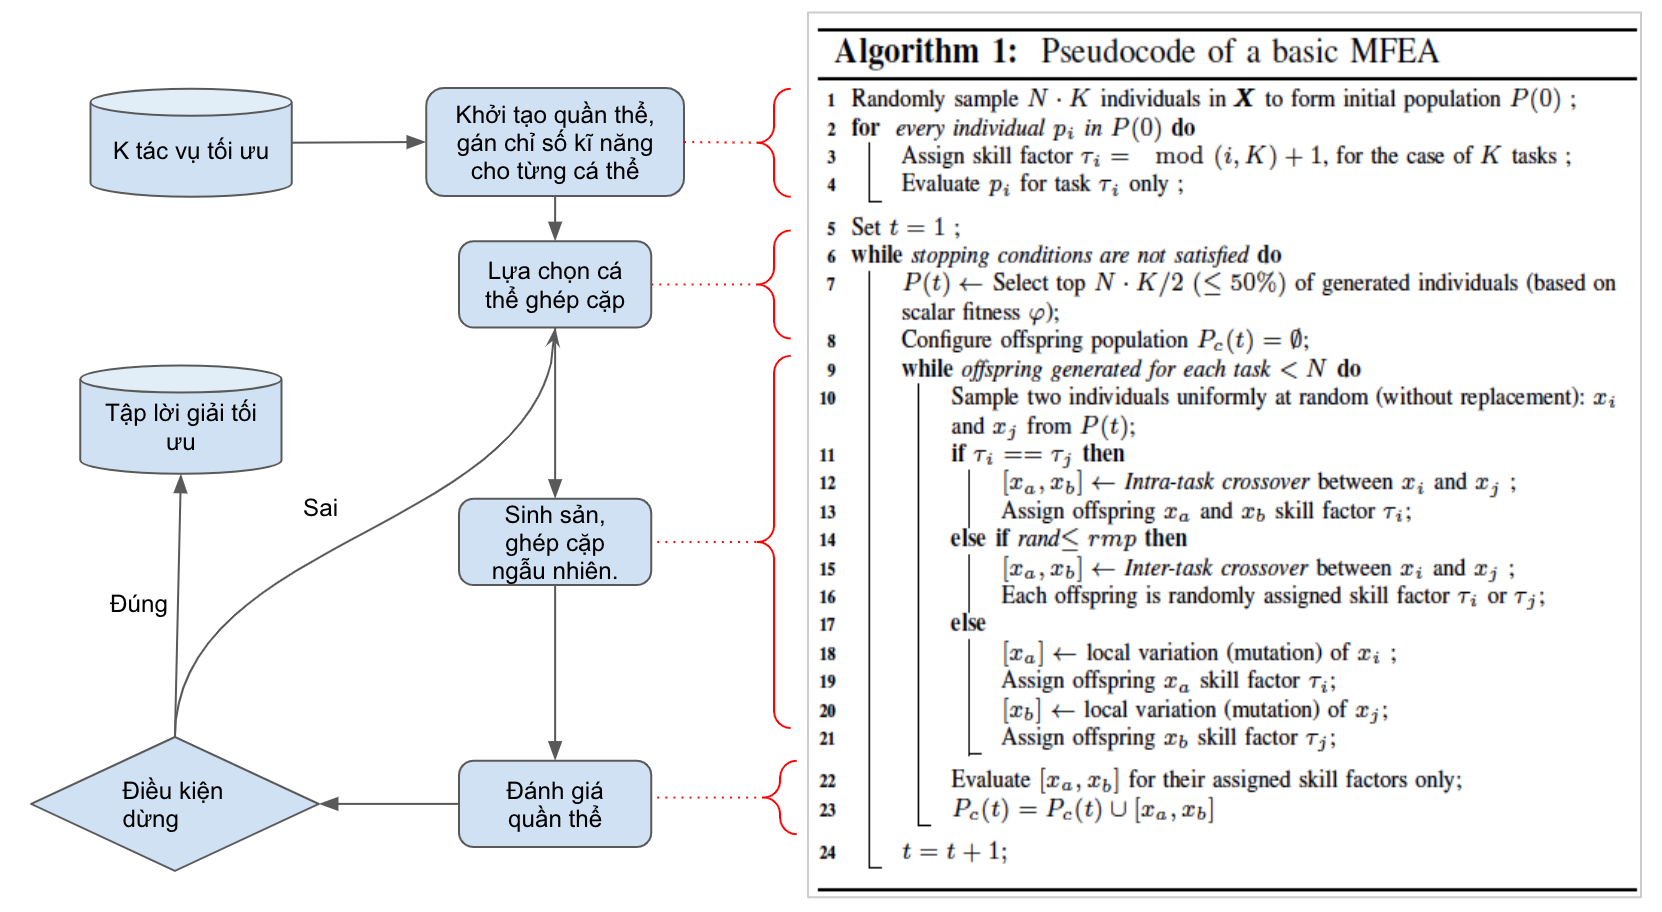
\includegraphics[width=0.85\linewidth]{thesis/images/mfea-alg.png}}
    \caption{Lược đồ giải thuật tiến hóa đa nhiệm MFEA-I \cite{gupta2016multifactorial}}
    \label{mfea-flow}
\end{figure}

Trong đó điểm khác biệt lớn nhất của MFEA-I so với thuật toán tiến hóa thông thường được mô tả tại \ref{section:cea} là cho phép lai ghép cá thể của các bài toán khác nhau theo một xác suất ghép cặp ngẫu nhiên (thuật ngữ gốc: \emph{random mating propability - rmp}). Phép lai ghép ngẫu nhiên đa nhiệm này đem đến một khả năng chia sẻ các gen tốt gữa các bài toán tối ưu hóa để đồng thời giải quyết cùng lúc chúng với tốc độ hội tụ nhanh hơn. 

Tuy nhiên, liệu việc kết hợp các lời giải của các bài toán tối ưu hóa khác nhau thì có sinh ra lời giải tốt hay không? Hoặc ít nhất cũng cần chỉ ra được trong trường hợp nào thì tốt, trường hợp nào thì không tốt. Các mục tiếp theo trong đồ án sẽ làm rõ hơn về vấn đề này.


    \section{Bài toán huấn luyện mạng neural}
        \begin{frame}{Cảm hứng từ sinh học}
        \begin{columns}
        \column{0.5\textwidth}
		\begin{itemize}
    		\begin{block}{Nền tảng}
    		    \begin{itemize}
    		    \item Được gọi là các mạng Nơ-ron nhân tạo, mô phỏng tổ chức thần kinh tự nhiên.
    		    \item Các nơ-ron đơn lẻ được gọi là các perceptron
    		    \item Thực chất là các mô hình toán học đơn giản định nghĩa một hàm $f: X \rightarrow Y$
    		    \end{itemize}
    		\end{block}
    		\begin{block}{Ứng dụng}
    		    \begin{itemize}
    		    \item Là cốt lõi của các mô hình Học sâu như CNN, RNN vv...
    		    \item Các bài toán hệ thống tự nhận diện, điều khiển, khai phá dữ liệu vv...
    		    \end{itemize}
    		\end{block}
		\end{itemize}
		\column{0.48\textwidth}
		\begin{figure}[ht]
            \centering
            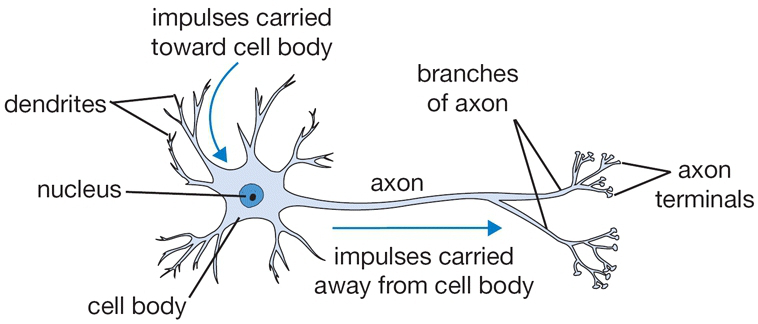
\includegraphics[width=1.0\linewidth]{images/neuron-net.png}
            \caption{Nơ-ron sinh học}
            \label{fig:problem:neural-architect}
            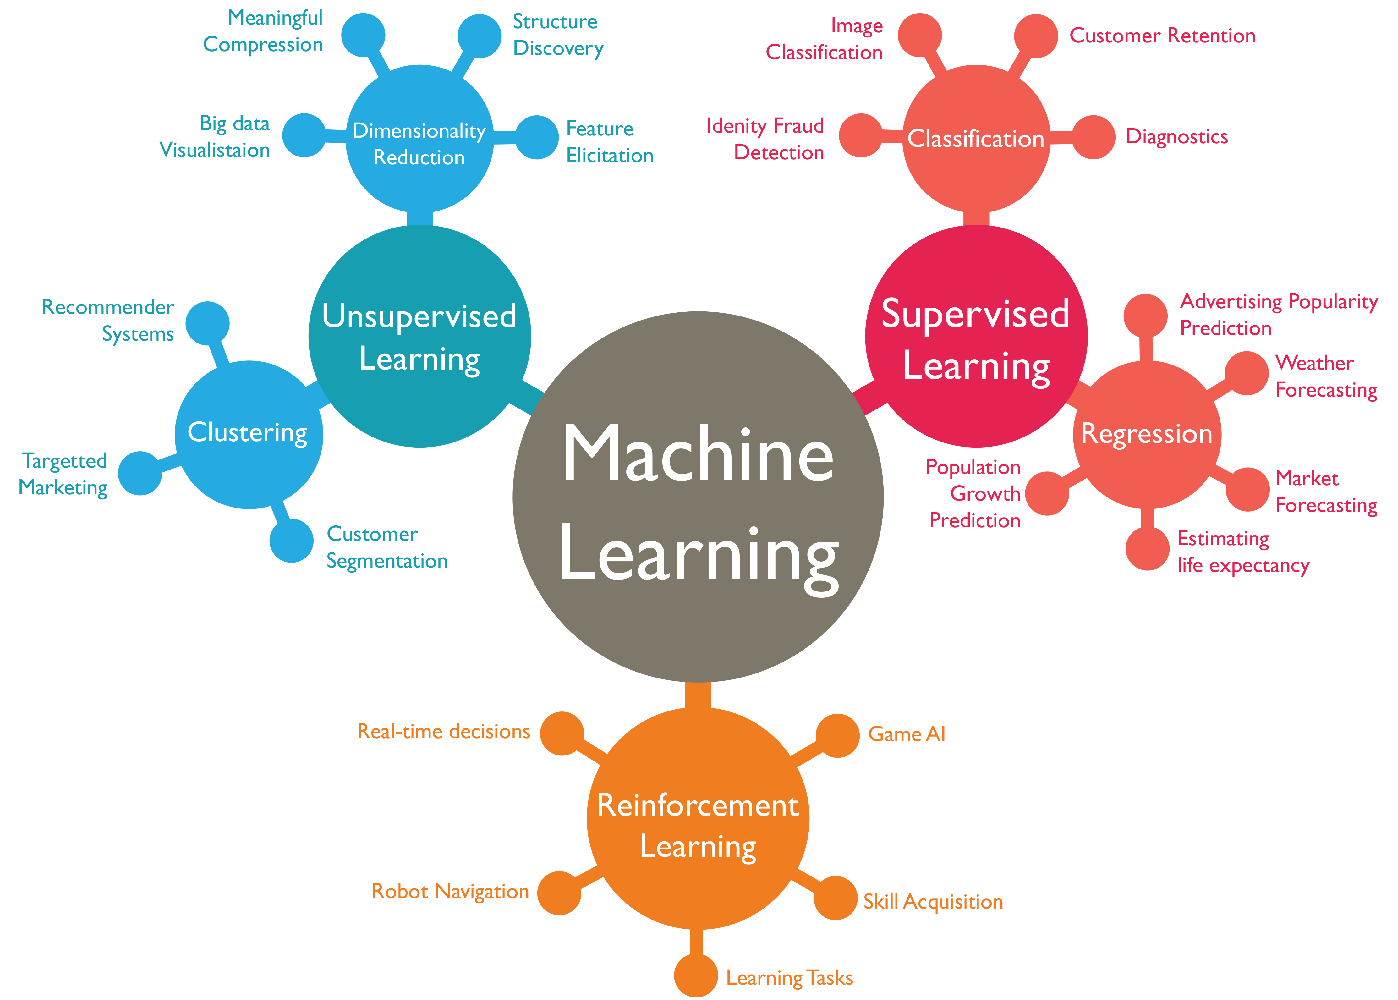
\includegraphics[width=1.0\linewidth, height=3cm]{images/machine.png}
            \caption{Học máy}
        \end{figure}
        
		\end{columns}
	\end{frame}
	
	\begin{frame}{Kiến trúc mạng Nơ-ron}
        \begin{columns}
        \column{0.45\textwidth}
		\begin{itemize}
    		\begin{block}{Kiến trúc mạng Nơ-ron}
    		     \emph{Perceptron} đa tầng: \emph{Lớp Input, Lớp Hidden, Lớp Output}.
    		\end{block}
    		\begin{block}{Mạng Nơ-ron lan truyền tiến}
    		    Mỗi nốt ở tầng nào đó sẽ nhận đầu vào từ các nốt ở tầng trước đó mà không có chiều suy luận ngược lại:
    		    \begin{equation}
                  \begin{array}{l}
                    z_i^{l+1} = \sum_{j=1}^{n^{(l)}}w_{ij}^{(l+1)}a_j^{(l)} + b_j^{(l+1)} \\
                    \\
                    a_i^{(l+1)} = g(z_i^{(l+1)})
                  \end{array}
                \end{equation}
                \textbf{Hàm chi phí:} $C: F \rightarrow R$ sao cho lời giải tối ưu $f^*, C(f^*)  \leq C(f) \forall f \in F$
    		\end{block}
		\end{itemize}
		\column{0.53\textwidth}
		\begin{figure}[ht]
            \centering
            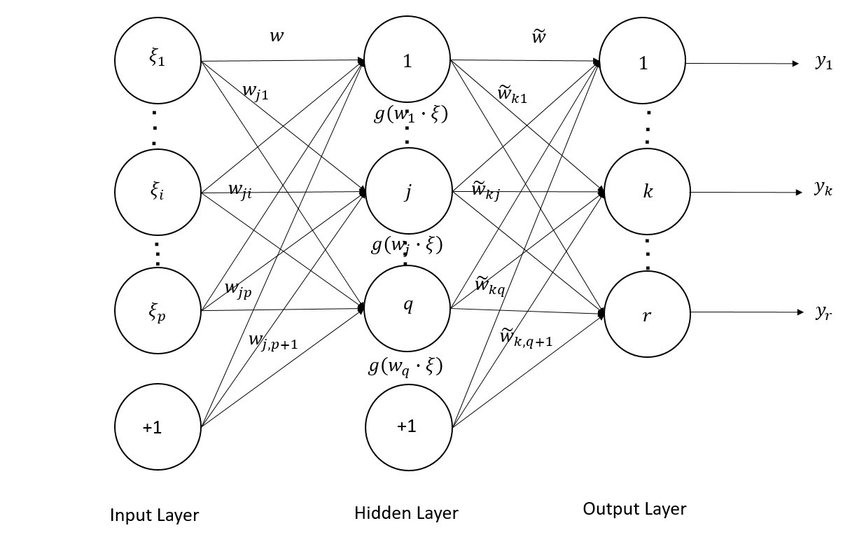
\includegraphics[width=1.0\linewidth, height=4.8cm]{images/ff-neural.png}
            \caption{Kiến trúc mạng Nơ-ron}
            \label{fig:problem:neural-architect}
        \end{figure}
		\end{columns}
	\end{frame}
	\begin{frame}{Huấn luyện mạng Nơ-ron}
	    \begin{itemize}
	    \begin{block}{Phương pháp huấn luyện}
        		    Có 2 lớp phương pháp chính
		    \begin{enumerate}
		        \setlength\itemsep{0.01em}
		        \item Lớp thuật toán sử dụng phương pháp \textbf{gradient-based}.
		        \item Lớp thuật toán \textbf{tiến hóa - NeuroEvolution}.
		    \end{enumerate}
		\end{block}
		\end{itemize}
        \begin{columns}
            \column{.6\linewidth}
    		\begin{itemize}
        		\begin{block}{Phương pháp Gradient}
        		    \begin{itemize}
        		    \item Cho hàm số $f(x), x\in \mathbb{R}$, $x^*$ là tối ưu cục bộ, $x_t$ gần $x^*$, tại đó $f^{'}(x_t) > 0$ thì cách tốt nhất để tìm điểm tối ưu là cập nhật $x_t$ ngược hướng đạo hàm:
        		    \begin{center}
        		        $x_{t+1}=x_t - \eta f^'(x_t)$ với $\eta$ là \textbf{tốc độ học}
        		    \end{center}
        		    \item \textcolor{blue}{Tổng quát với hàm nhiều biến $f(\theta)$}:
        		    \begin{center}
                         $\theta_{t+1} = \theta_t - \eta \bigtriangledown_\theta f(\theta_t)$
                    \end{center}\\
                    \end{itemize}
        		\end{block}
        	\end{itemize}
        	\column{.4\linewidth}
        	    \begin{figure}[ht]
                    \centering
                    \fbox{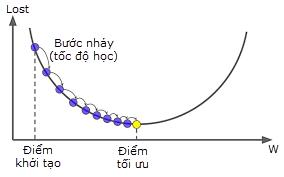
\includegraphics[width=0.7\linewidth]{images/gd.jpg}}
                    \caption{Minh họa cách cập nhật tham số của GD}
                    \label{fig:gd}
                \end{figure}
        \end{columns}
	\end{frame}
	\begin{frame}{Gradient Based và EA}
	    \begin{block}{Gradient Based và EA}
		    Phương pháp dựa trên gradient-based cho đến nay được sử dụng rộng rãi tuy nhiên đang gặp phải một số hạn chế nhất định.
		    \begin{itemize}
		        \setlength\itemsep{0.01em}
		        \item Với những bài toán mà kết quả đầu ra khó xác định, việc tính toán hàm lỗi để cập nhật tham số vô cùng khó khăn.
		        \item Với những mô hình đơn giản nhiều khả năng dẫn tới \emph{cực trị địa phương}.
		    \end{itemize}
		    Vì điều này nhiều nhóm nghiên cứu bắt đầu áp dụng \textbf{EA} để giải quyết các bài toán của mình như \emph{Google Brain, OpenAI, Uber}.  
		\end{block}\pause
		\begin{block}{}
		    \textcolor{red}{Vậy thì huấn luyện mạng Nơ-ron sử dụng EA (NeuroEvolution) hoạt động như thế nào?}
		\end{block}
	\end{frame}
	\begin{frame}{Tiến hóa trong mạng Nơ-ron}
		\begin{itemize}
    		\begin{block}{NeuroEvolution - Khái quát}
    		\begin{itemize}
    		    \setlength\itemsep{0.01em}
    		    \item Được xem xét dưới dạng bài toán tối ưu hộp đen (blackbox optimization)
    		    \item Kiểu gen (genotype) là kiểu cá thể của quần thể sẽ được ánh xạ với các tham số trong mạng Nơ-ron được đánh giá qua hàm \emph{fitness} tương ứng.
    		    \end{itemize}
    		    Vấn đề: \textcolor{red}{Không khai thác được những tri thức đã học được trong các mô hình đã học được trước đó.}
    		\end{block}\pause
    		\begin{block}{Đề xuất: Tiến hóa đa nhiệm trong mạng Nơ-ron}
    		\begin{itemize}
    		    \setlength\itemsep{0.01em}
    		    \item Khai thác mối quan hệ tiềm ẩn của các mạng, tăng tốc độ hội tụ lẫn nhau.
    		    \item Chia thành 2 loại tác vụ tương ứng với các bài toán riêng biệt:
    		    \begin{enumerate}
    		        \setlength\itemsep{0.01em}
    		        \item Mỗi tác vụ tương ứng với một bộ \textbf{\textcolor{red}{dữ liệu, đặc tính dữ liệu}} khác nhau. Ví dụ: bài toán Cart-Pole với môi trường có gravity = 9.8 và gravity = 19.8?
    		        \item Mỗi tác vụ tương ứng với một \textbf{\textcolor{red}{cấu trúc mạng}} khác nhau. Ví dụ: Mô hình mạng với lớp ẩn có 10 nơ-ron và mô hình mạng lớp ẩn 12 nơ-ron.
    		    \end{enumerate}
    		\end{itemize}
    		\textcolor{red}{Trong phạm vi đồ án sẽ giải quyết lần lượt cả 2 bài toán trên}
    		\end{block}
        \end{itemize}
	\end{frame}
	\begin{frame}{Bài toán huấn luyện mạng Nơ-ron}
	    \begin{figure}[ht]
            \centering
            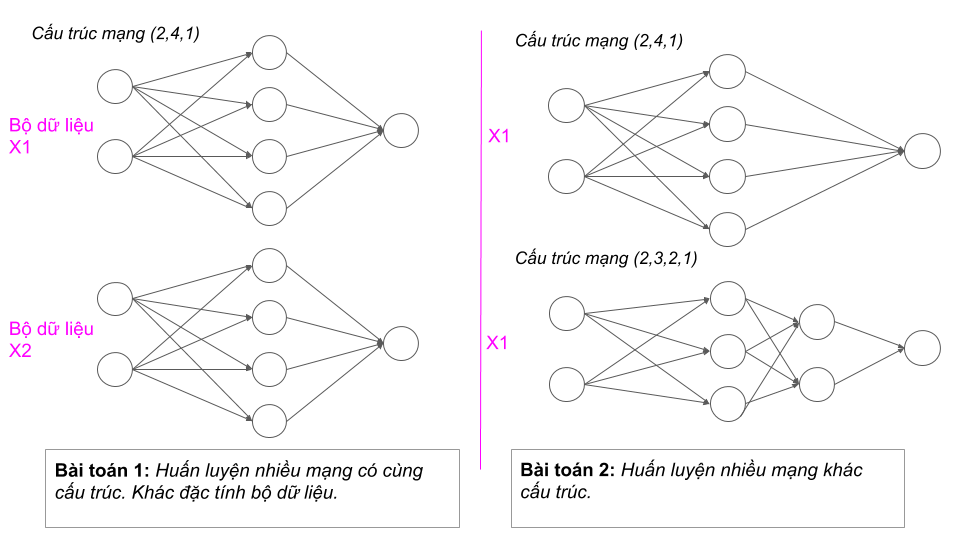
\includegraphics[width=1.0\linewidth]{images/neural-problem.png}
            \caption{Bài toán huấn luyện mạng Nơ-ron}
            \label{fig:problem:neural-problem}
        \end{figure}
	\end{frame}
    \section{Huấn luyện nhiều mạng neural đa cấu trúc}
    	\begin{frame}{Động lực}
	    \begin{columns}
	    \column{0.57\textwidth}
		\begin{itemize}
		    \begin{block}{Cảm hứng từ tự nhiên}
		        \begin{itemize}
		            \item Bộ não tự nhiên của con người là một cấu trúc mô-đun phức tạp.
		            \item Khi xử lý một công việc có thể sử dụng kinh nghiệm khi đã làm một công việc tương tự.
		        \end{itemize}
		    \end{block}\pause
		    \begin{block}{Vấn đề: Mạng Nơ-ron có cấu trúc mô-đun}
		        \begin{itemize}
		            \item Nhiều mạng nơ-ron có số nút trong lớp ẩn khác nhau. 
		            \item Mạng nhỏ sẽ được sử dụng như một phần của mạng lớn.
		        \end{itemize}
		        Động lực: \textcolor{red}{Để tận dụng tri thức đã học khi cấu trúc mạng thay đổi.}
		    \end{block}
		\end{itemize}
		\column{0.4\textwidth}
		\begin{figure}[ht]
            \centering
            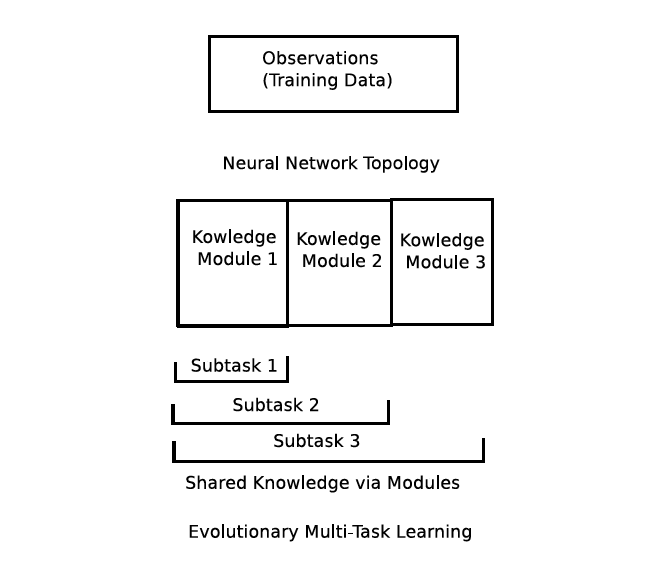
\includegraphics[width=1.2\linewidth]{images/modular.png}
            \caption{Mô hình biểu diễn mạng nơ-ron mô-đun hóa}
            \label{fig:problem:modular}
        \end{figure}
		\end{columns}
	\end{frame}
	
	\begin{frame}{Huấn luyện nhiều mạng Nơ-ron đa cấu trúc}
		\begin{itemize}
		    \begin{block}{Vấn đề}
		        \textcolor{red}{Khi cấu trúc mạng thay đổi không tận dụng được tri thức đã học từ cấu trúc mạng trước đó. Hoặc khi muốn tìm cấu trúc mạng tối ưu cho một bài toán.}
		    \end{block}
		    \begin{block}{Phát biểu bài toán}
		        \begin{itemize}
		            \item Cho $K$ tác vụ $T_1, T_2, ... T_K$ với $j \in [1,K]$.
		            \item Mỗi tác vụ tương đương với một bài toán tối ưu hóa 1 cấu trúc mạng nơ-ron lần lượt là $h_1, h_2, ... , h_K$ khác nhau.
		        \end{itemize}
		        Mục tiêu: \textcolor{red}{Khai thác mối quan hệ tiềm ẩn, tối ưu hóa đồng thời $K$ tác vụ.}
		    \end{block}
		\end{itemize}
	\end{frame}
	
	\begin{frame}{Giải thuật tiến hóa đề xuất}
	    \begin{itemize}
		    \begin{block}{Huấn luyện nhiều mạng nơ-ron có cấu trúc mô-đun}
		        \begin{enumerate}
		            \setlength\itemsep{0.01em}
		            \item Coi cấu trúc mạng được coi là một tác vụ tối ưu
		            \item Sử dụng thuật toán tiến hóa đa nhiệm MFEA-I, MFEA-II.
		            \item Đánh giá từng cá thể của tác vụ tương ứng với cấu trúc mạng nơ-ron của nó
		        \end{enumerate}
		        Vấn đề: \textcolor{red}{Mã hóa, giải mã từng cá thể để phù hợp với các cấu trúc mạng nơ-ron riêng biệt}
		    \end{block}
		    \begin{block}{Đề xuất}
		        \begin{enumerate}
		            \setlength\itemsep{0.01em}
		            \item Không gian biểu diễn chung cho các cấu trúc mạng kich thước $D$.
		            \item Thuật toán mã hóa, giải mã các cá thể:
		            \begin{itemize}
		                \setlength\itemsep{0.01em}
		                \item Mã hóa: Các tham số $(w,b)$ được mã hóa "gián tiếp" vào véc-tơ có kích thước $D$.
		                \item Giải mã: Từ cá thể có kích thước $D$ trả về bộ tham số $(w,b)$ tính giá trị hàm lỗi tương ứng.
		            \end{itemize}
		        \end{enumerate}
		    \end{block}
		\end{itemize}
	\end{frame}
	\begin{frame}{Mô tả thuật toán}
	    \begin{itemize}
		    \begin{block}{Giả định}
		        \begin{itemize}
	                \setlength\itemsep{0.01em}
	                \item Cho $K$ tác vụ $T_1, T_2, ... ,T_k$ với $j \in [1,K]$. Mỗi tác vụ tương đương với một mô hình mạng neural có số lượng lớp ẩn và số lượng nút tại lớp ẩn khác nhau. 
                    \item Định nghĩa $l_j$ là số lượng lớp trong cấu trúc mạng của tác vụ $T_j$, $h_j^{(i)}$ là số lượng nút tại lớp ẩn thứ i của tác vụ $T_j$ với  $j \in [1,K]$ và  $i \in [1,l_j]$.
                    % \item Định nghĩa $\theta = \max_{j \in [1,K]}l_j$ là số lượng lớp lớn nhất trong tất cả các tác vụ. Vậy $h_{multitask}^{\theta} = \max_{j \in [1,K]}h_j^{(l_j)}$ là số lượng nút lớn nhất ở lớp cuối cùng của tất cả các tác vụ. 
	            \end{itemize}
		    \end{block}
		    \begin{block}{Thuật toán}
		        \begin{enumerate}
		            \item Tính $H_{multitask}$ bao gồm tất cả các tham số của không gian tìm kiếm chung.
		            Khởi tạo không gian tìm kiếm chung với kích thước:\\
		            $D_{unified} = \sum_{l={1,...L}}h_{l-1}h_l + h_l$ từ ma trận $H_{multitask}$.
                    \item Khởi tạo $W_{multitask}$, Danh sách các ma trận trọng số tương ứng với $H_{multitask}$.
                    \item Tính $W_{j}$, tương ứng với ma trận trọng số $h_{j}$ với $j \in \{1, ..,K\}$
		        \end{enumerate}
		    \end{block}
		\end{itemize}
	\end{frame}
	
	\begin{frame}{Ví dụ}
	    \begin{block}{}
	        \textcolor{blue}{Bài toán: } Giả sử ta có 3 tác vụ có cấu trúc mạng tương ứng với $H_1 = [2, 2, 2, 1]$, $H_2 = [2, 3, 2, 1]$ và $H_3 = [2, 3, 1]$. Áp dụng thuật toán mã hóa, giải mã với các tác vụ này
	    \end{block}
	    \begin{block}{Tính $H_{multitask}$ và không gian biểu diễn chung}
	        \begin{columns}
	        \column{0.5\linewidth}
	        \begin{enumerate}
	            \setlength\itemsep{0.01em}
	            \item Tính $H_{multitask}$: $H_{multitask}=[2, 3, 3, 1]$ \Rightarrow Tổng số tham số: $D_{unified} = \sum_{l={1,...L}}h_{l-1}h_l + h_l$ \Rightarrow \textbf{25 tham số}.
	            \item Một kiểu gen (genotype) được biểu diễn dưới dạng:
	            \centerline{$
                  genotype=
                  \begin{bmatrix}
                    1& 2& 3& \dots & 25
                  \end{bmatrix}
                $}
	        \end{enumerate}
	        \column{0.5\linewidth}
	        \begin{figure}[]
                    \centering
                    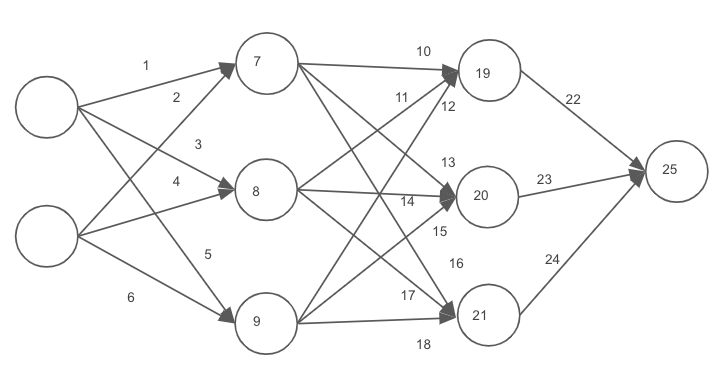
\includegraphics[width=1.0\linewidth]{images/neural-ex1.png}
                    \caption{Mạng Nơ-ron biểu diễn chung}
                    \label{fig:problem:neural-ex1}
            \end{figure}
	        \end{columns}
	    \end{block}
    \end{frame}
%     \begin{frame}{Ví dụ (2)}
% 		    \begin{block}{Bước 2: Tính danh sách ma trận trọng số: $W_{multitask}$}
% 		        \begin{columns}
% 		            \column{0.3\textwidth}
% 		            Lớp 1:
% 		            \begin{equation*}
% 		            \\
% 		              \begin{array}{l}
%                       W_1=
%                       \begin{bmatrix}
%                         1& 3& 5\\
%                         2& 4& 6
%                       \end{bmatrix}\\
%                       \\
%                       b_1=
%                       \begin{bmatrix}
%                         7& 8& 9
%                       \end{bmatrix}
%                     \end{array}

%                     \end{equation*}
                    
%                     \column{0.3\textwidth}
%                     Lớp 2:
%                     \begin{align*}
%                     \begin{array}{l}
%                       W_2=
%                       \begin{bmatrix}
%                         10& 13& 16\\
%                         11& 14& 17\\
%                         12& 15& 18
%                       \end{bmatrix}\\
%                       \\
%                       b_2=
%                       \begin{bmatrix}
%                         19& 20& 21\\
%                       \end{bmatrix}
%                       \end{array}
%                     \end{align*}
%                     \column{0.3\textwidth}
%                     Lớp 3:
%                     \begin{align*}
%                     \begin{array}{l}
%                       W_3=
%                       \begin{bmatrix}
%                         22\\
%                         23\\
%                         24
%                       \end{bmatrix}\\
%                       \\
%                       b_3=
%                       \begin{bmatrix}
%                         25
%                       \end{bmatrix}
%                       \end{array}
%                     \end{align*}
% 		        \end{columns}
% 		    \end{block}
% 	\end{frame}
% 	\begin{frame}{Bước 3: Giải mã bộ trọng số $W_j$, $b_j$ trên mỗi tác vụ}
%     		    \begin{columns}
%         		\column{0.3\textwidth}
%         		    \begin{block}{Task1: $H_1 = [2, 2, 2, 1]$}
%         		    \begin{equation*}
%         		      \begin{array}{l}
        		      
%                       W_1=
%                       \begin{bmatrix}
%                         1& 3\\
%                         2& 4
%                       \end{bmatrix},\\
%                       \\
%                       b_1=
%                       \begin{bmatrix}
%                         7& 8
%                       \end{bmatrix}
%                       \end{array}
%                     \end{equation*}
                
%                     \begin{equation*}
%                     \begin{array}{l}
%                       W_2=
%                       \begin{bmatrix}
%                         10& 13\\
%                         11& 14
%                       \end{bmatrix},\\
%                       \\
%                       b_2=
%                       \begin{bmatrix}
%                         19& 20\\
%                       \end{bmatrix}
%                       \end{array}
%                     \end{equation*}
%                     \begin{equation*}
%                     \begin{array}{l}
%                       W_3=
%                       \begin{bmatrix}
%                         22\\
%                         23
%                       \end{bmatrix},\\
%                       \\
%                       b_3=
%                       \begin{bmatrix}
%                         25
%                       \end{bmatrix}
%                       \end{array}
%                     \end{equation*}
%                 \end{block}
                    
%         	\column{0.3\textwidth}
%         		\begin{block}{Task2: $H_2 = [2, 3, 2, 1]$}
%                 \begin{equation*}
%                 \begin{array}{l}
%                   W_1=
%                   \begin{bmatrix}
%                     1& 3& 5\\
%                     2& 4& 6
%                   \end{bmatrix},\\
%                   \\
%                   b_1=
%                   \begin{bmatrix}
%                     7& 8& 9
%                   \end{bmatrix}
%                   \end{array}
%                 \end{equation*}
            
%                 \begin{equation*}
%                 \begin{array}{l}
%                   W_2=
%                   \begin{bmatrix}
%                     10& 13\\
%                     11& 14\\
%                     12& 15
%                   \end{bmatrix},\\
%                   \\
%                   b_2=
%                   \begin{bmatrix}
%                     19& 20\\
%                   \end{bmatrix}
%                   \end{array}
%                 \end{equation*}
            
            
%                 \begin{equation*}
%                 \begin{array}{l}
%                   W_3=
%                   \begin{bmatrix}
%                     22\\
%                     23
%                   \end{bmatrix},\\
%                   \\
%                   b_3=
%                   \begin{bmatrix}
%                     25
%                   \end{bmatrix}
%                   \end{array}
%                 \end{equation*}
%                 \end{block}
%         		\column{0.3\textwidth}
        		
%         		\begin{block}{Task3: $H_3 = [2, 3, 1]$}
%                 \begin{equation*}
%                 \begin{array}{l}
%                   W_1=
%                   \begin{bmatrix}
%                     1& 3& 5\\
%                     2& 4& 6
%                   \end{bmatrix},\\
%                   \\
%                   b_1=
%                   \begin{bmatrix}
%                     7& 8& 9
%                   \end{bmatrix}
%                   \end{array}
%                 \end{equation*}
            
%                 \begin{equation*}
%                 \begin{array}{l}
%                   W_2=
%                   \begin{bmatrix}
%                     22\\
%                     23\\
%                     24
%                   \end{bmatrix},\\
%                   \\
%                   b_2=
%                   \begin{bmatrix}
%                     25
%                   \end{bmatrix}
%                   \end{array}
%                 \end{equation*}
%                 \end{block}
%     		    \end{columns}
% 	\end{frame}
	\begin{frame}{Ví dụ: Trực quan các bước}
		\begin{figure}[h!] 
            \centering
            \fbox{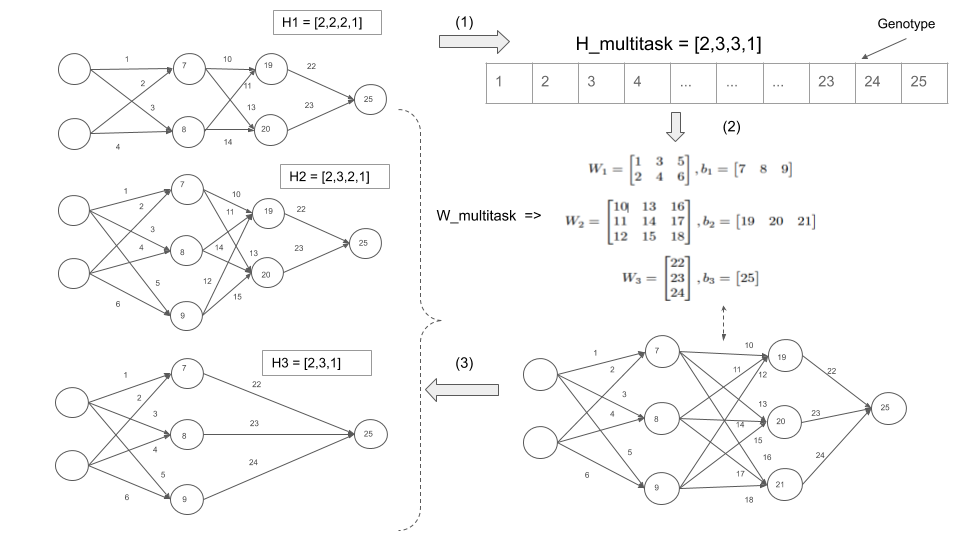
\includegraphics[width=1.0\linewidth, height=6cm]{images/modular-ex.png}}
            \caption{Ví dụ thuật toán đề xuất cho các mô hình mạng H1(2,2,2,1), H2(2,3,2,1), H3(2,3,1)}
            \label{fig:problem:modular-ex1}
        \end{figure}
	\end{frame}
	\begin{frame}{Mã hóa, giải mã cá thể}
	    \begin{figure}[]
            \centering
            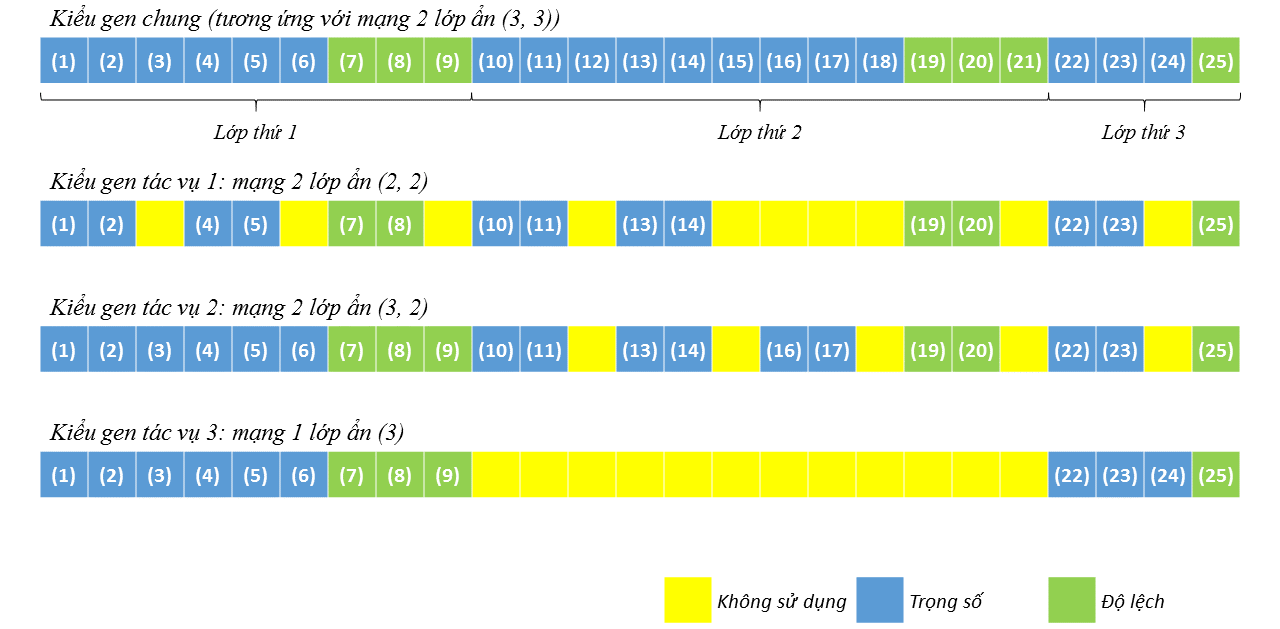
\includegraphics[width=1.0\linewidth]{images/neural-decode.jpg}
            \caption{Biểu diễn không gian chung và biểu diễn từng cá thể}
            \label{fig:problem:neural-ex1}
        \end{figure}
        \textit{Sử dụng phép lai ghép SBX, PMU thông thường, phù hợp với giả thiết parent-centric}.
	\end{frame}
    \section{Huấn luyện nhiều mạng neural trên các môi trường khác nhau}
    	\begin{frame}{Nền tảng Học tăng cường}
		\begin{columns}
		\column{0.6 \textwidth}
        \begin{itemize}
    		\begin{block}{Khái quát học tăng cường (Reinforcement Learning)}
    		    \begin{itemize}
    		    \setlength\itemsep{0.01em}
    		    \item Một kiểu học máy chính bên cạnh học có giám sát và học không giám sát.
    		    \item 2 đối tượng chính: tác nhân - \emph{Agent} và môi trường - \emph{Environment}.
    		    \item Mục tiêu: Tác nhân thu được tổng phần thưởng lớn nhất khi tương tác với mối trường qua các hành động.
    		    \end{itemize}
    		    \textcolor{blue}{Thành phần chính}:
    		    \begin{itemize}
    		        \setlength\itemsep{0.01em}
        		    \item \textbf{policy function}: Ánh xạ từ tập trạng thái của môi trường đến tập hành động.
        		    \item \textbf{reward}: Phần thưởng qua mỗi hành động của tác nhân.
        		    \item \textbf{value function}: Tổng phần thưởng dự kiến của agent.
    		    \end{itemize}
    		\end{block}
		\end{itemize}
		\column{0.4 \textwidth}
		\begin{figure}[ht]
            \fbox{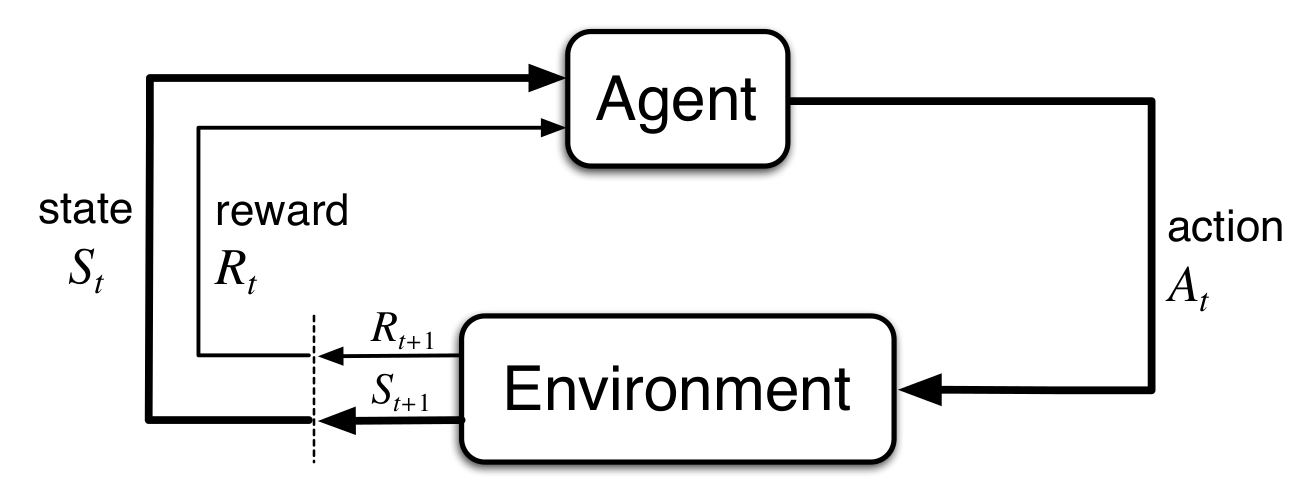
\includegraphics[width=0.9\linewidth]{images/mdp.png}}
            \caption{Chu trình học trong học tăng cường. Quá trình quyết định Markov}
            \label{fig:problem:mdp}
        \end{figure}
		\end{columns}
	\end{frame}
	\begin{frame}{Huấn luyện mô hình học tăng cường}
		\begin{columns}
		\column{0.6 \textwidth}
        \begin{itemize}
    		\begin{block}{Phương pháp}
    		    \begin{itemize}
    		    \setlength\itemsep{0.01em}
    		    \item Sử dụng \emph{tabular methods}. Chỉ phù hợp với mô hình đơn giản.
    		    \item Tối ưu hóa hàm mục tiêu \emph{policy function}, \emph{value function}
    		    \end{itemize}
    		\end{block}
    		\begin{block}{Tối ưu hóa \emph{policy function} sử dụng mạng Nơ-ron}
    		    \begin{itemize}
    		    \setlength\itemsep{0.01em}
    		    \item Coi \emph{policy function} là một mạng nơ-ron.
    		    \item Đầu vào của mạng là trạng thái của \emph{environment}. Đầu ra của mạng là \emph{action} của \emph{agent}.
    		    \item Phần thưởng thu được chính là độ đo để đánh giá chất lượng của mô hình mạng.
    		    \end{itemize}
    		\end{block}
		\end{itemize}
		\column{0.4 \textwidth}
		\begin{figure}[ht]
            \centering
            \fbox{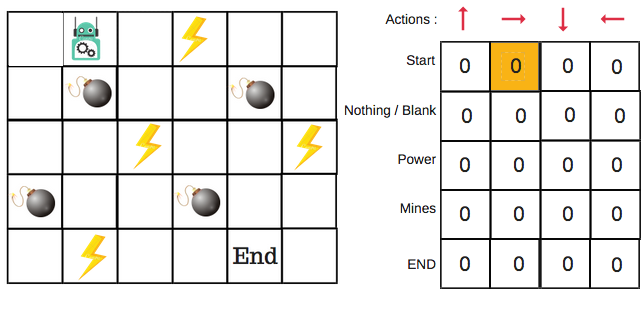
\includegraphics[width=0.9\linewidth]{images/tabular-table.png}}
            \caption{Tabular Methods}
            \label{fig:problem:tabular}
            \fbox{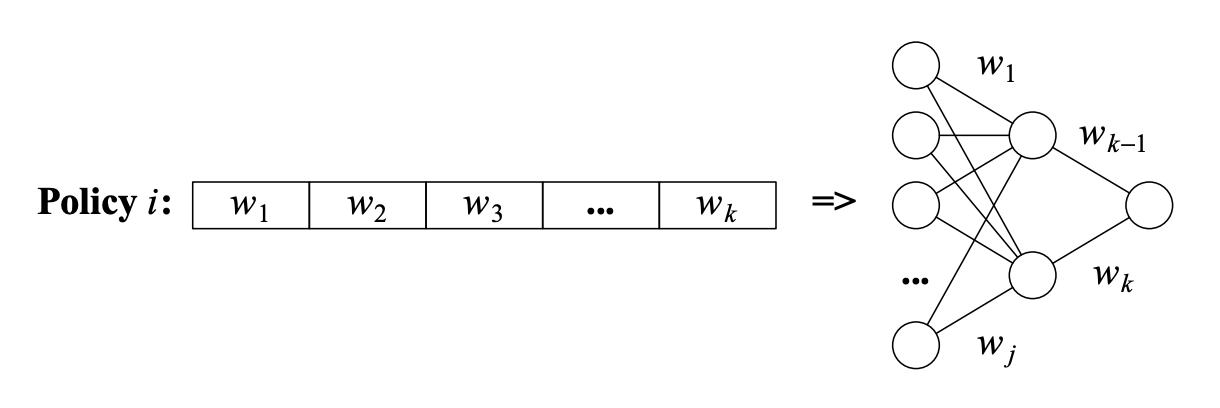
\includegraphics[width=0.9\linewidth]{images/policy.png}}
            \caption{Biểu diễn policy}
        \end{figure}
		\end{columns}
	\end{frame}
	
	\begin{frame}{Vấn đề khi huấn luyện policy function}
	    \begin{itemize}
	    \begin{block}{Vấn đề}
	    \textcolor{red}{Khi thông số môi trường thay đổi thì trạng thái cũng thay đổi theo. \emph{Policy} tối ưu vừa học không còn phù hợp, phải huấn luyện lại từ đầu.}
	    \end{block}
	    \begin{block}{Phát biểu bài toán}
	        \begin{itemize}
    		    \setlength\itemsep{0.01em}
    		    \item Cho $K$ tác vụ $T_1, T_2, ..., T_K$.
    		    \item Giả sử $h_k$ là bộ tham số môi trường tương ứng với tác vụ $T_k$, $h_j$ là bộ tham số môi trường tương ứng với tác vụ $T_j$ và $h_j \neq h_k$.
    		    \end{itemize}
    		    Mục tiêu: 
    		    \begin{itemize}
    		        \item Mỗi tác vụ được biểu diễn bởi một mạng Nơ-ron.
    		        \item Khai thác mối quan hệ tiềm ẩn, tối ưu hóa đồng thời $K$ tác vụ.
    		    \end{itemize}
	    \end{block}
	    \end{itemize}
	\end{frame}
	
	\begin{frame}{Tối ưu hóa đa nhiệm nhiều mạng policy}
	    \begin{itemize}
    	    \begin{block}{Giả định}
    	    \begin{itemize}
    	        \item Mỗi tác vụ là một nhiệm vụ tối ưu \emph{policy}, tương đương với việc tối ưu một mạng nơ-ron.
    	        \item Các mạng nơ-ron có cùng cấu trúc.
    	        \item Bộ dữ liệu đầu vào của mỗi mạng là tương đối khác nhau do thay đổi tham số môi trường.
    	    \end{itemize}
    	    \end{block}
    	    \begin{block}{Giải quyết}
    	    \begin{itemize}
    	        \item Áp dụng mô hình thuật toán tối ưu hóa đa nhiệm.
    	        \item Mỗi cá thể được mã hóa, giải mã bằng phương pháp mã hóa, giải mã đề xuất.
    	        \item Hàm đánh giá là tổng phần thưởng \emph{agent} nhận với mô hình policy trong tác vụ tương ứng
    	    \end{itemize}
    	    \end{block}
	    \end{itemize}
	\end{frame}
	
	\begin{frame}{Phương pháp tiến hóa đề xuất tối ưu policy function}
		\begin{columns}
		\column{0.5 \textwidth}
        \begin{itemize}
    		\begin{block}{Mã hóa và giải mã nhiễm sắc thể}
    		    \begin{itemize}
    		    \setlength\itemsep{0.01em}
    		    \item Các tham số trong mạng lần lượt được mã hóa "trực tiếp" vào nhiễm sắc thể.
    		    \item Quá trình giải mã ngược lại để đánh giá mô hình mạng.
    		    \end{itemize}
    		\end{block}
    		\begin{block}{Áp dụng EA để huấn luyện mạng}
    		    \begin{itemize}
    		    \setlength\itemsep{0.01em}
    		    \item \emph{fitness} của cá thể là tổng phần thưởng thu được từ mô hình hiện tại.
    		    \item Mô hình policy càng tối ưu thì tổng phần thưởng thu được càng cao.
    		    \end{itemize}
    		\end{block}
		\end{itemize}
		\column{0.48 \textwidth}
		\begin{figure}[ht]
            \centering
            \fbox{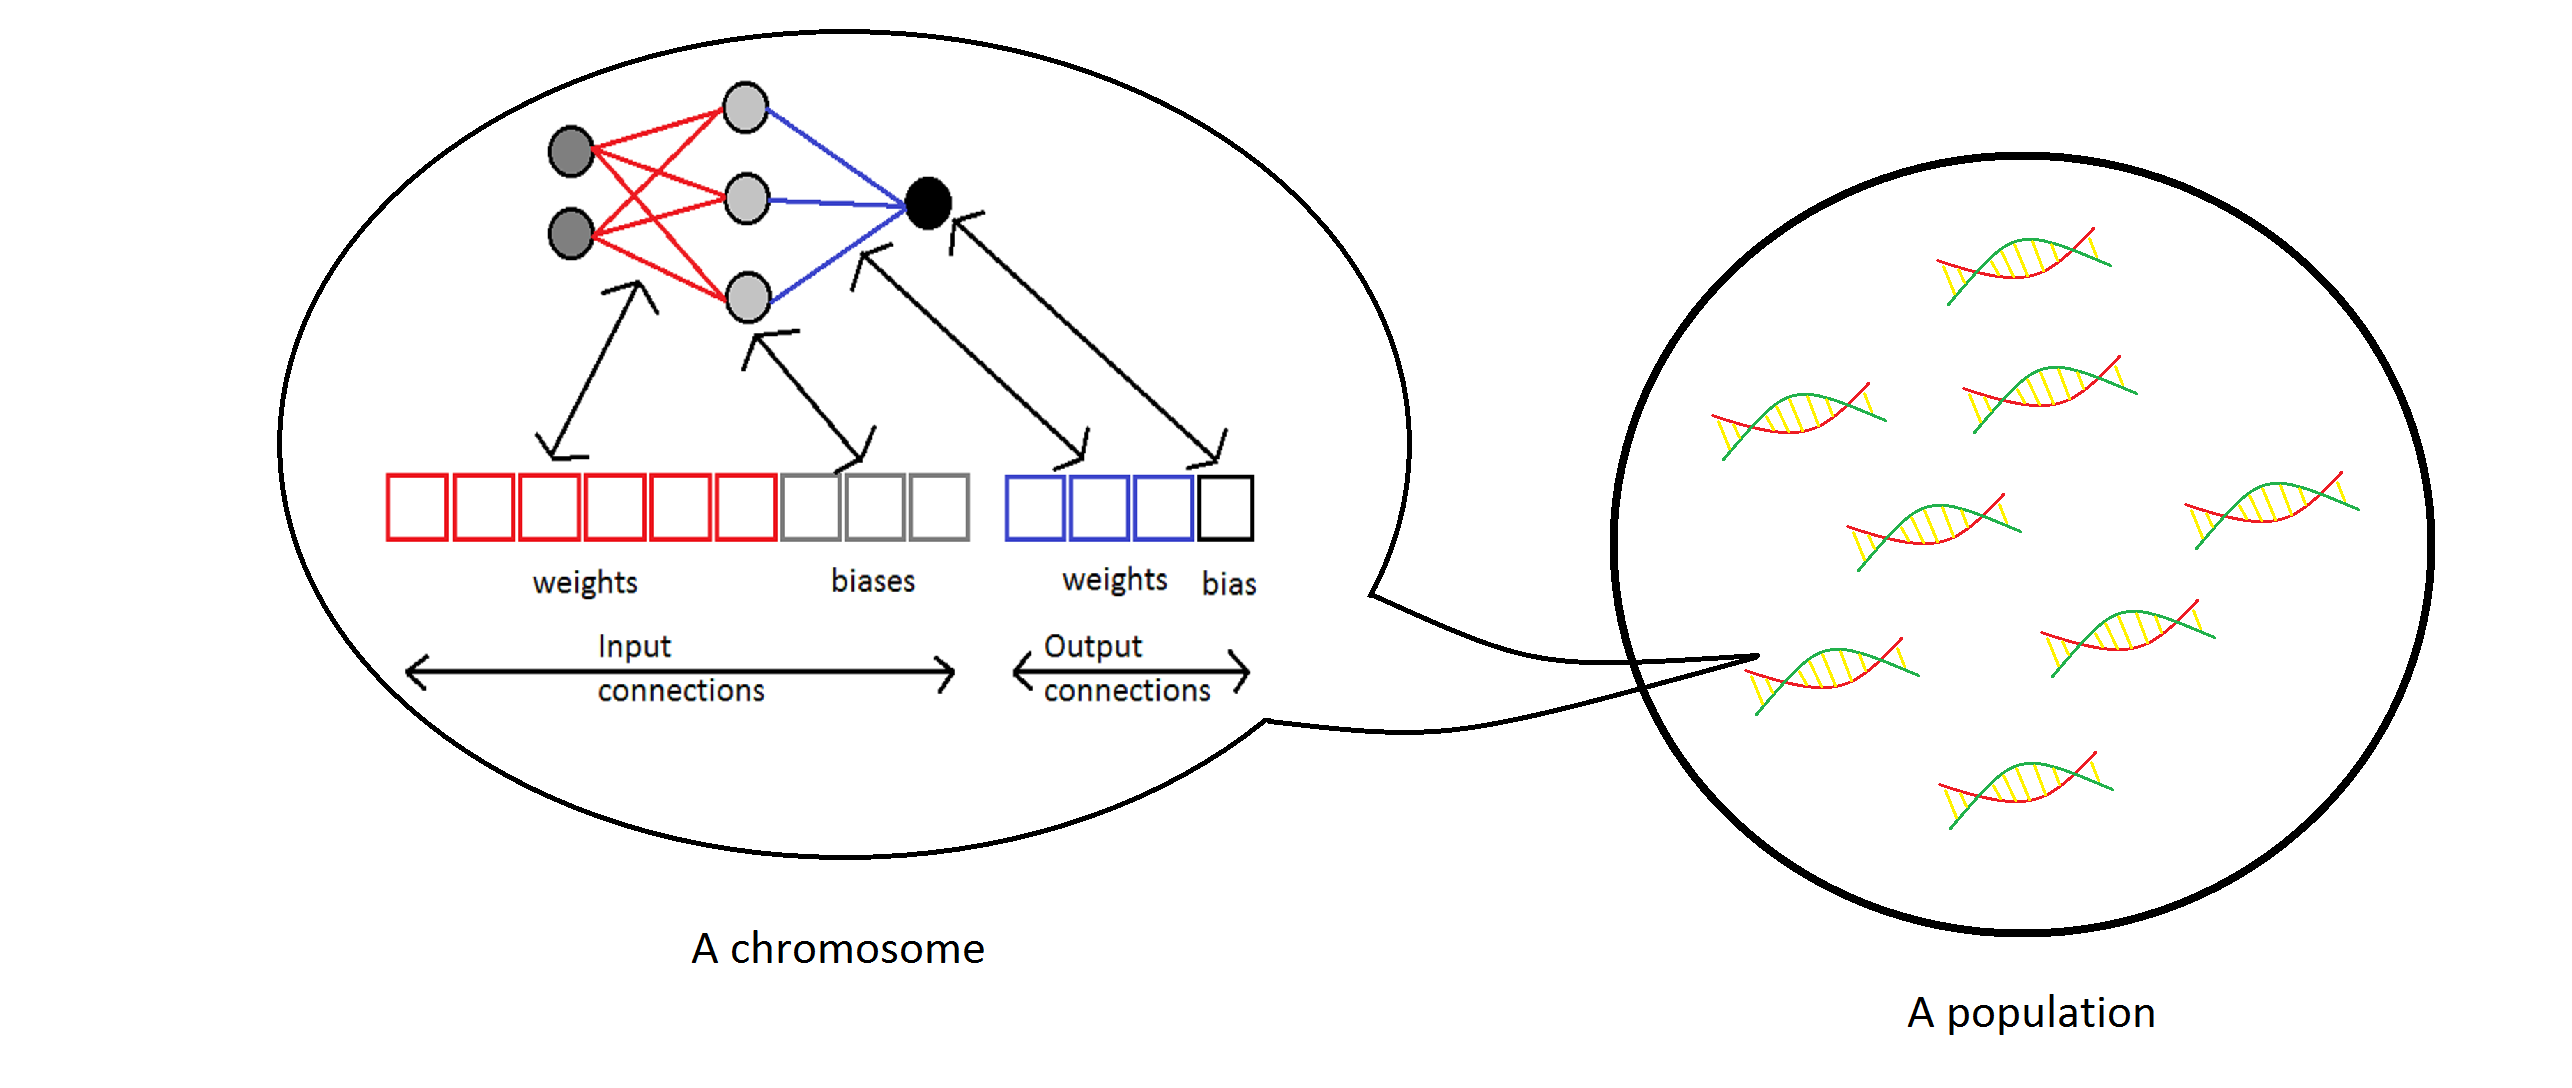
\includegraphics[width=0.95\linewidth]{images/proposed_encoding.png}}
            \caption{Mã hóa và giải mã policy.}
            \label{fig:problem:policy}
            \fbox{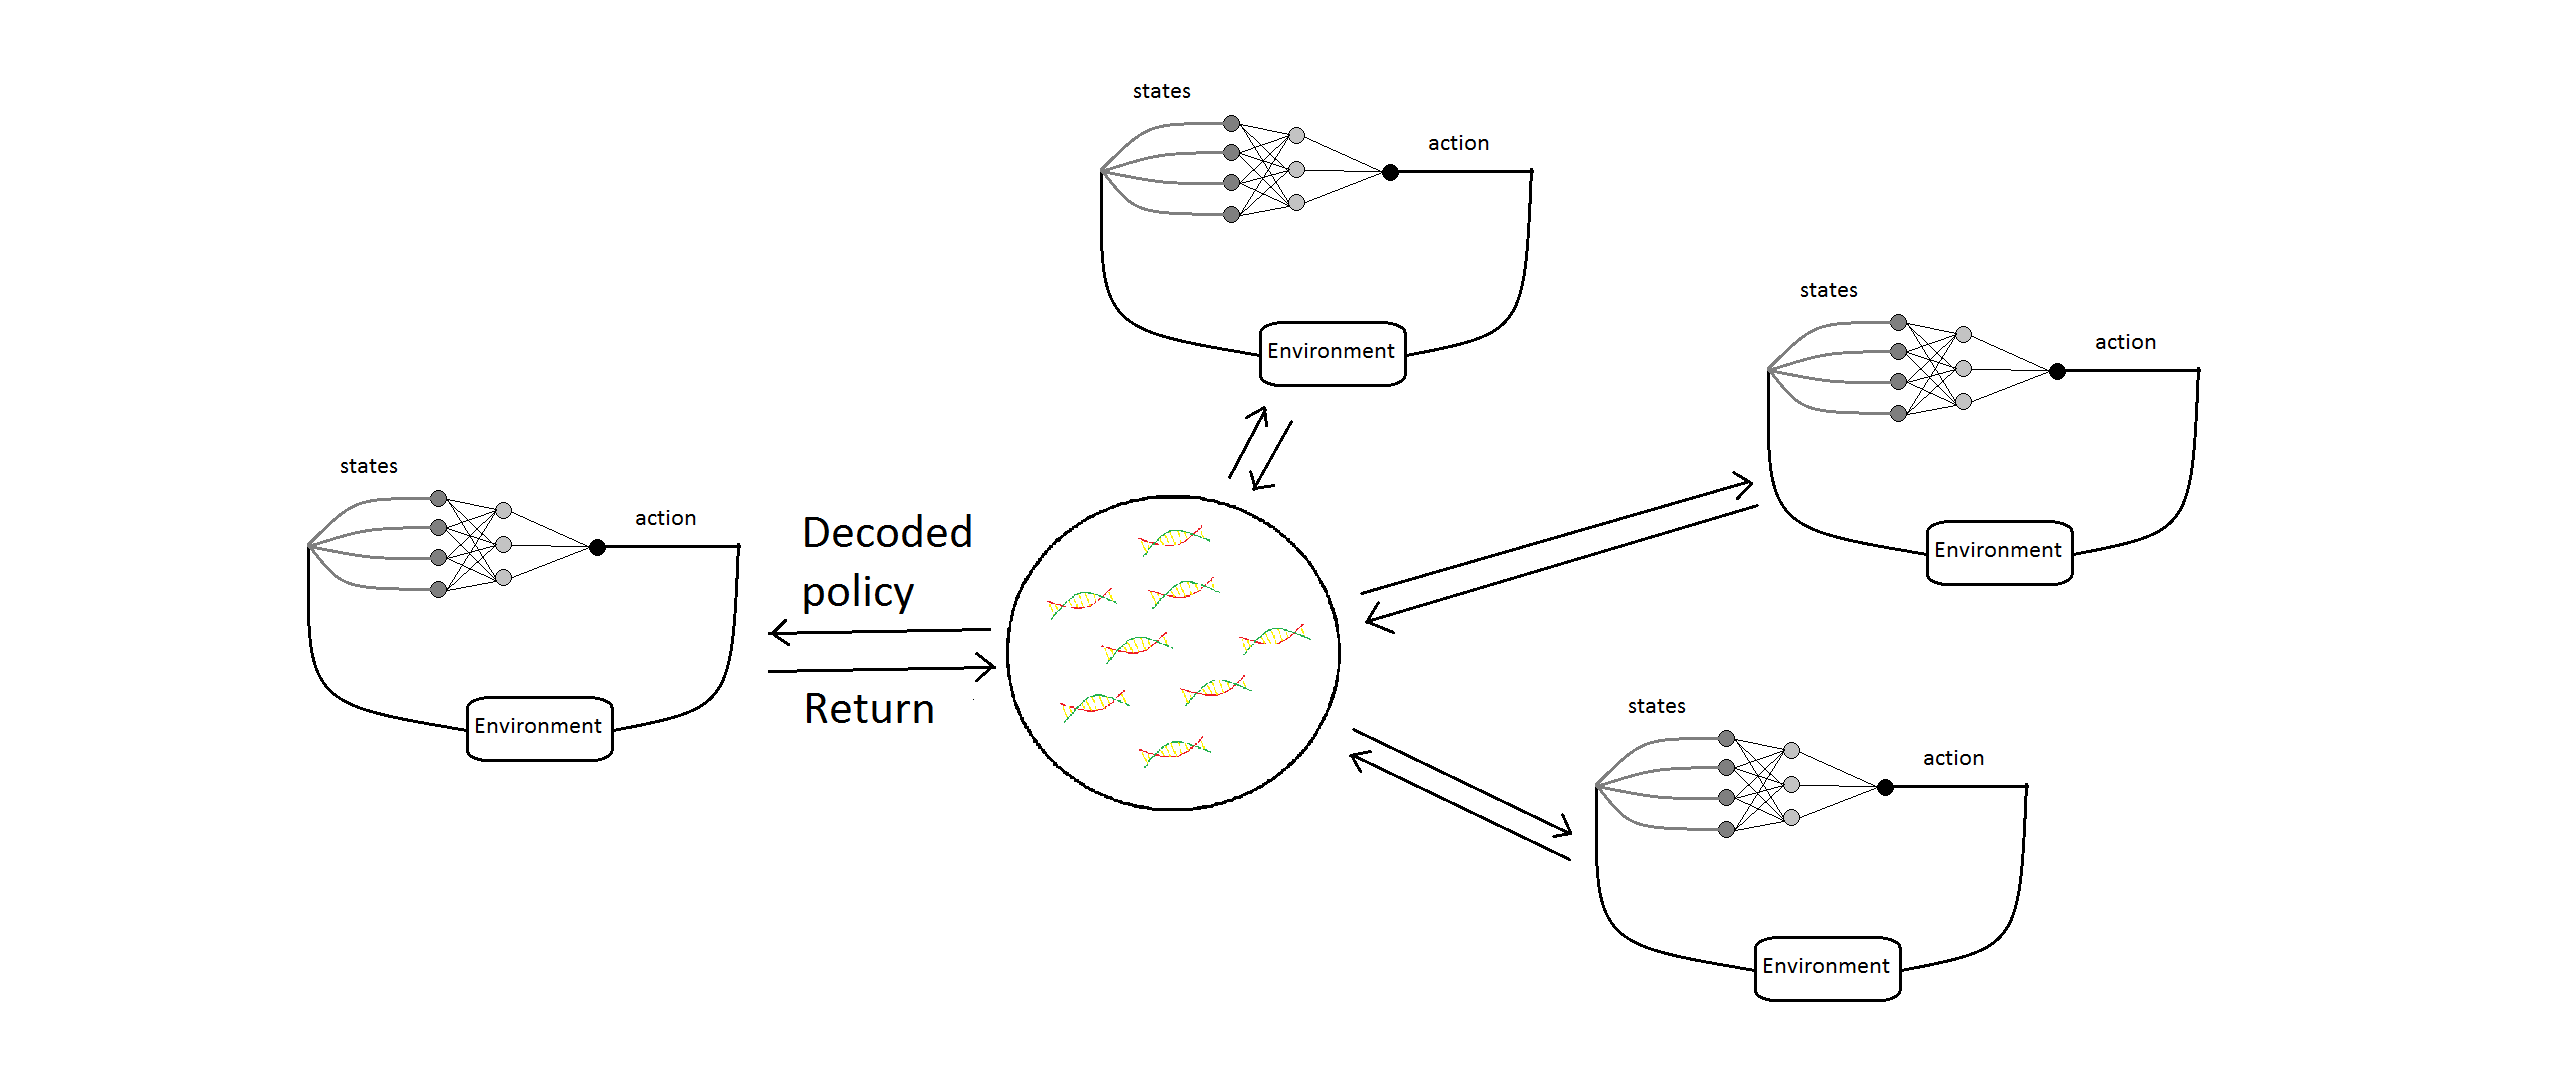
\includegraphics[width=0.95\linewidth]{images/proposed_ea.png}}
            \caption{Toàn cảnh dùng EA để tối ưu hóa policy}
        \end{figure}
		\end{columns}
	\end{frame}
    \section{Kết quả thực nghiệm}
    
\subsection{Huấn luyện nhiều mô mạng neural đa lớp}
\subsubsection{Bảng kết quả thực nghiệm - mạng neural cùng độ sâu 1 lớp ẩn}

\begin{table} [H]
    \begin{center}
        \caption{Kết quả thực nghiệm bài 4-bit 1 lớp ẩn}

    \begin{tabular}{|c|c|c|c|}
    \hline
    \multirow{1}{*}{\textbf{Method}} & \multicolumn{1}{c|}{\textbf{Subtask1}} & \multicolumn{1}{c|}{\textbf{Subtask 2}} & \multicolumn{1}{c|}{\textbf{Subtask 3}} \\ \hline
    CEA & $0.0316 \pm 0.0125$ & $0.0201 \pm 0.011922$ & $0.0117 \pm 0.008133$ \\
    MFEA-I & $0.025 \pm 0.012957$ & $0.0117 \pm 0.007342$ & $0.0072 \pm 0.005355$\\
    MFEA-II  & $\mathbf{0.0219 \pm 0.009181}$ & $\mathbf{0.0099 \pm 0.007053}$ & $\mathbf{0.0052 \pm 0.004126}$ \\\hline
    
    \end{tabular}
    \end{center}
    
    \label{tab:result:nbit}
\end{table}
\begin{table} [H]   
    \begin{center}
        \caption{Kết quả thực nghiệm bài 6-bit 1 lớp ẩn}

    \begin{tabular}{|c|c|c|c|}
    \hline
    \multirow{1}{*}{\textbf{Method}} & \multicolumn{1}{c|}{\textbf{Subtask1}} & \multicolumn{1}{c|}{\textbf{Subtask 2}} & \multicolumn{1}{c|}{\textbf{Subtask 3}} \\ \hline
    CEA(5,6,7)  & $0.0703 \pm 0.014543$ & $0.0619 \pm 0.018078$ & $0.0572 \pm 0.017982$ \\
    MFEA-I(5,6,7)   & $\mathbf{0.06 \pm 0.014702}$ & $\mathbf{0.0498 \pm 0.009562}$ & $0.047 \pm 0.008464$ \\
    MFEA-II(5,6,7)  & $0.06 \pm 0.011387$ & $0.052 \pm 0.009393$ & $\mathbf{0.047 \pm 0.009579}$ \\\hline
    
    CEA(6,7,8)   & $0.0669 \pm 0.016032$ & $0.0583 \pm 0.009948$ & $0.0521 \pm 0.015598$ \\
    MFEA-I(6,7,8)  & $0.0611 \pm 0.013622$ & $0.0528 \pm 0.011122$ & $0.0484 \pm 0.011074$ \\
    MFEA-II(6,7,8) & $\mathbf{0.0522 \pm 0.011066}$ & $\mathbf{0.0476 \pm 0.01033}$ & $\mathbf{0.0418 \pm 0.011741}$ \\\hline
    
    \end{tabular}
    \end{center}
    \label{tab:result:nbit}
\end{table}    
\begin{table} [H]
    \begin{center}
        \caption{Kết quả thực nghiệm bài 8-bit 1 lớp ẩn}

    \begin{tabular}{|c|c|c|c|}
    \hline
    \multirow{1}{*}{\textbf{Method}} & \multicolumn{1}{c|}{\textbf{Subtask1}} & \multicolumn{1}{c|}{\textbf{Subtask 2}} & \multicolumn{1}{c|}{\textbf{Subtask 3}} \\ \hline
    CEA(5,6,7) & $0.0956 \pm 0.013764$ & $0.0906 \pm 0.015274$ & $0.0874 \pm 0.010884$ \\
    MFEA-I(5,6,7) & $0.0859 \pm 0.011722$ & $0.0801 \pm 0.009489$ & $0.0778 \pm 0.010507$  \\
    MFEA-II(5,6,7) & $\mathbf{0.0827 \pm 0.010678}$ & $\mathbf{0.076 \pm 0.012979}$ & $\mathbf{0.0735 \pm 0.012598}$ \\\hline
    
    CEA(6,7,8)& $0.0895 \pm 0.012499$ & $0.0902 \pm 0.013171$ & $0.081 \pm 0.013371$ \\
    MFEA-I(6,7,8)  & $0.0826 \pm 0.011089$ & $0.0768 \pm 0.010228$ & $0.0734 \pm 0.008805$ \\
    MFEA-II(6,7,8) & $\mathbf{0.0808 \pm 0.010726}$ & $\mathbf{0.0739 \pm 0.01117}$ & $\mathbf{0.072 \pm 0.009657}$ \\\hline
    \end{tabular}
    \end{center}
    \label{tab:result:nbit}
\end{table}

\subsubsection{Biểu đồ hội tụ - mạng neural cùng độ sâu 1 lớp ẩn}
\begin{figure}[H]
    \centering

    \scalebox{.7}{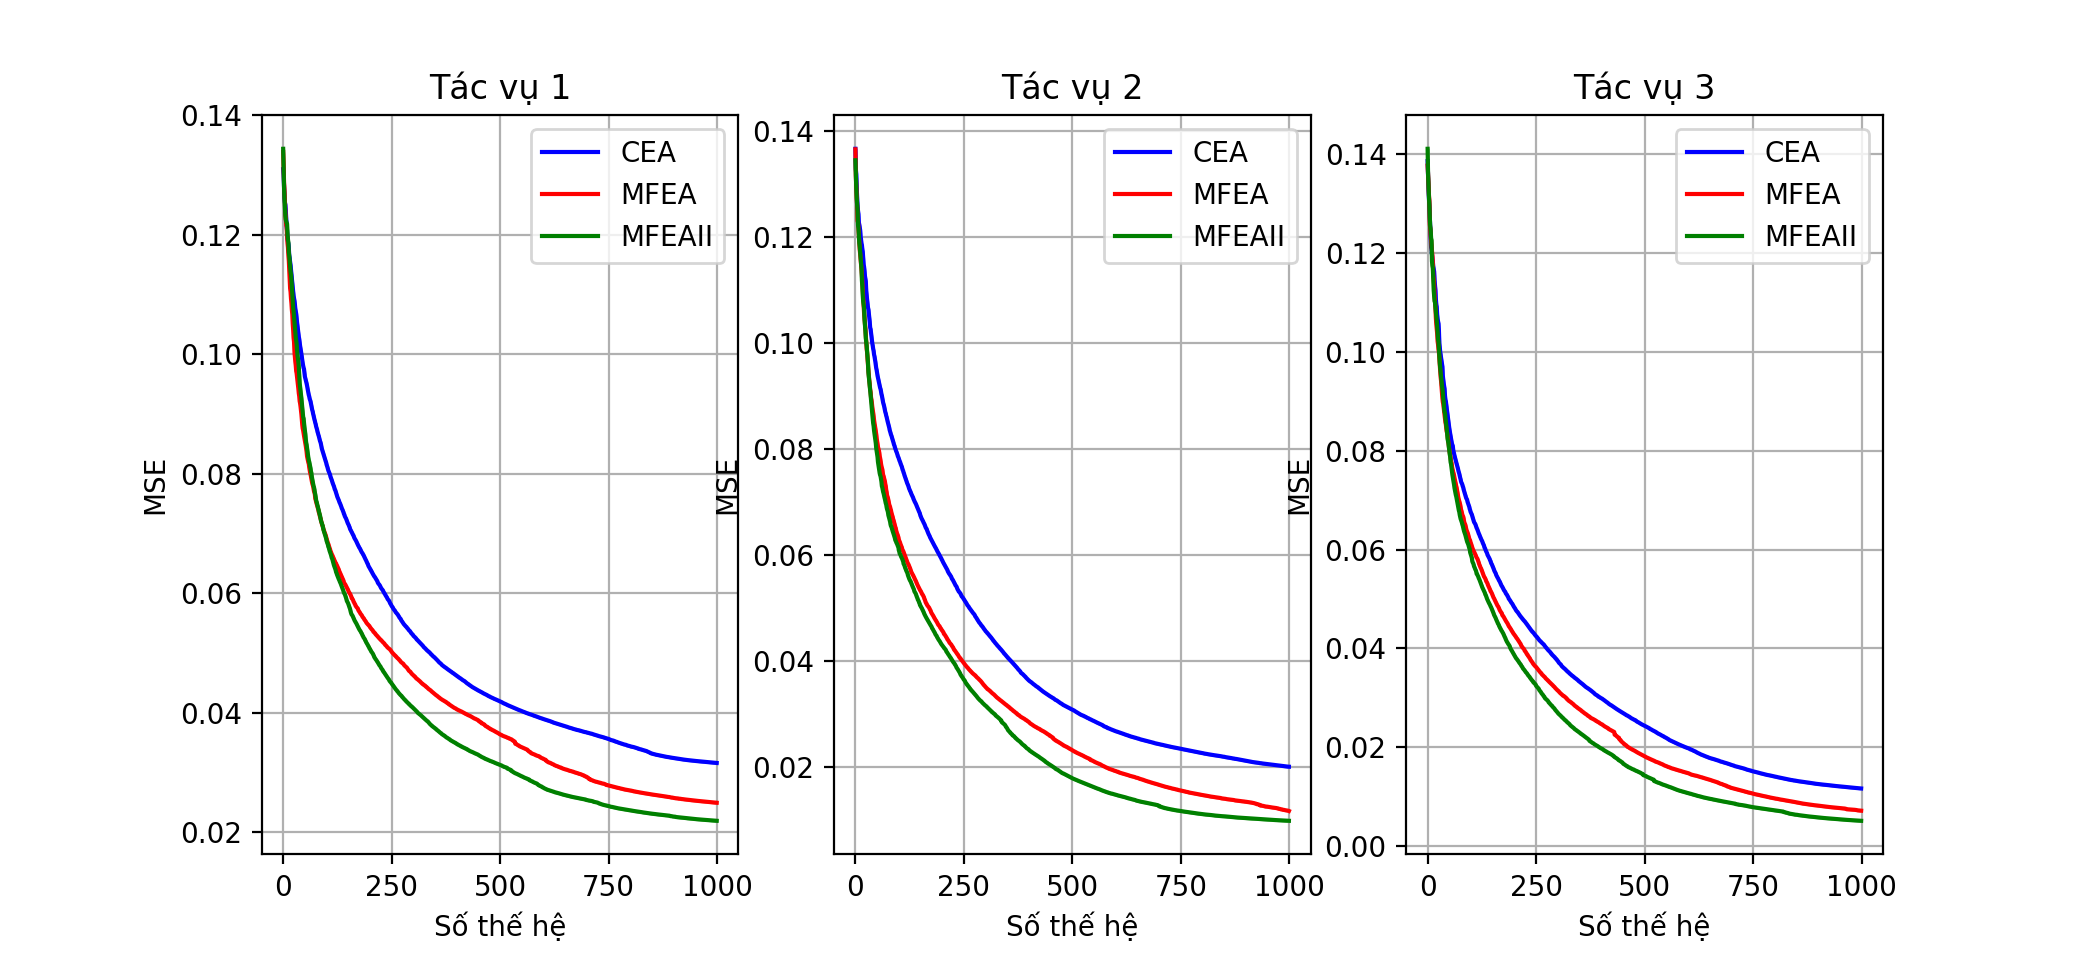
\includegraphics[width=\textwidth,height=\textheight,keepaspectratio]{thesis/images/results/nbit_1layer/4bit_task.png}}
    \scalebox{.7}{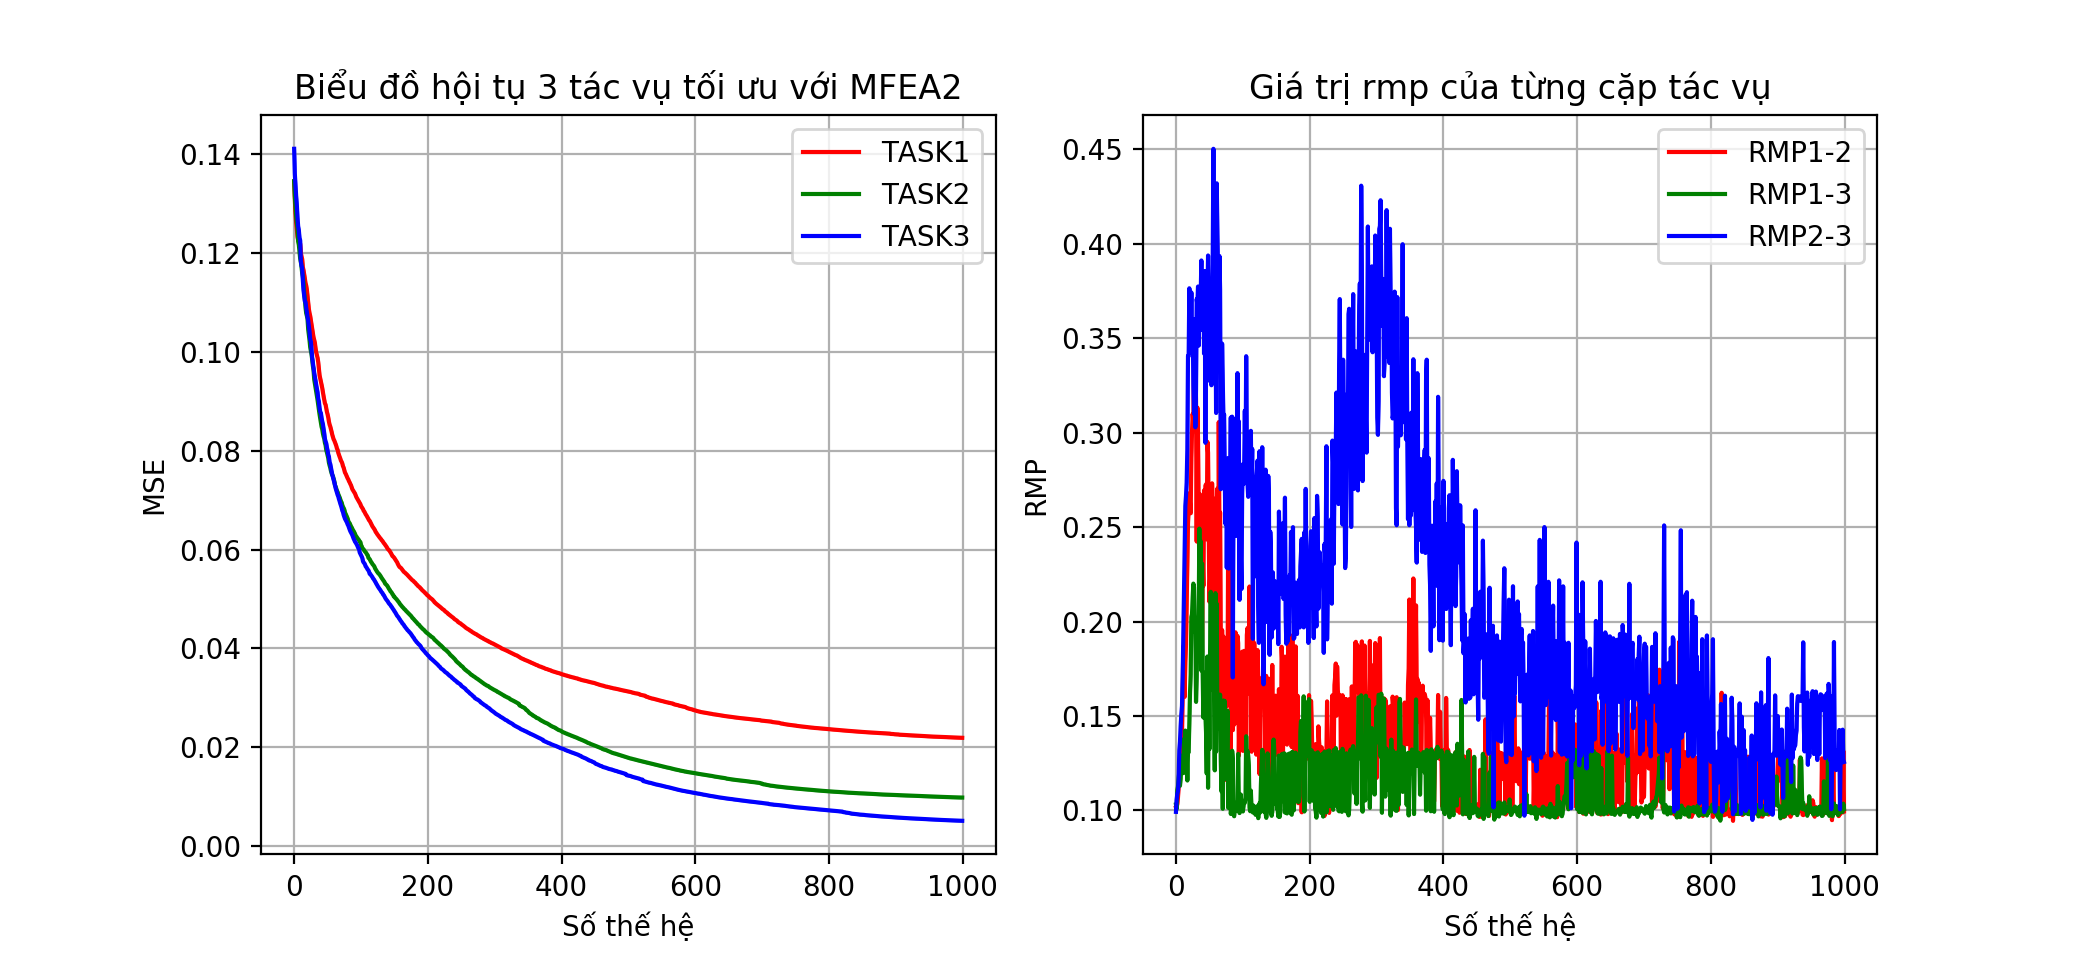
\includegraphics[width=\textwidth,height=\textheight,keepaspectratio]{thesis/images/results/nbit_1layer/4bit_rmp.png}}
    \label{fig:4bit_1layer}
    \caption{Bài 4bit: Biểu đồ hội tụ của từng tác vụ trên các thuật toán và biểu đồ phân tích MFEA-II theo giá trị rmp}

\end{figure}
\begin{figure}[H]
    \centering
    \scalebox{.7}{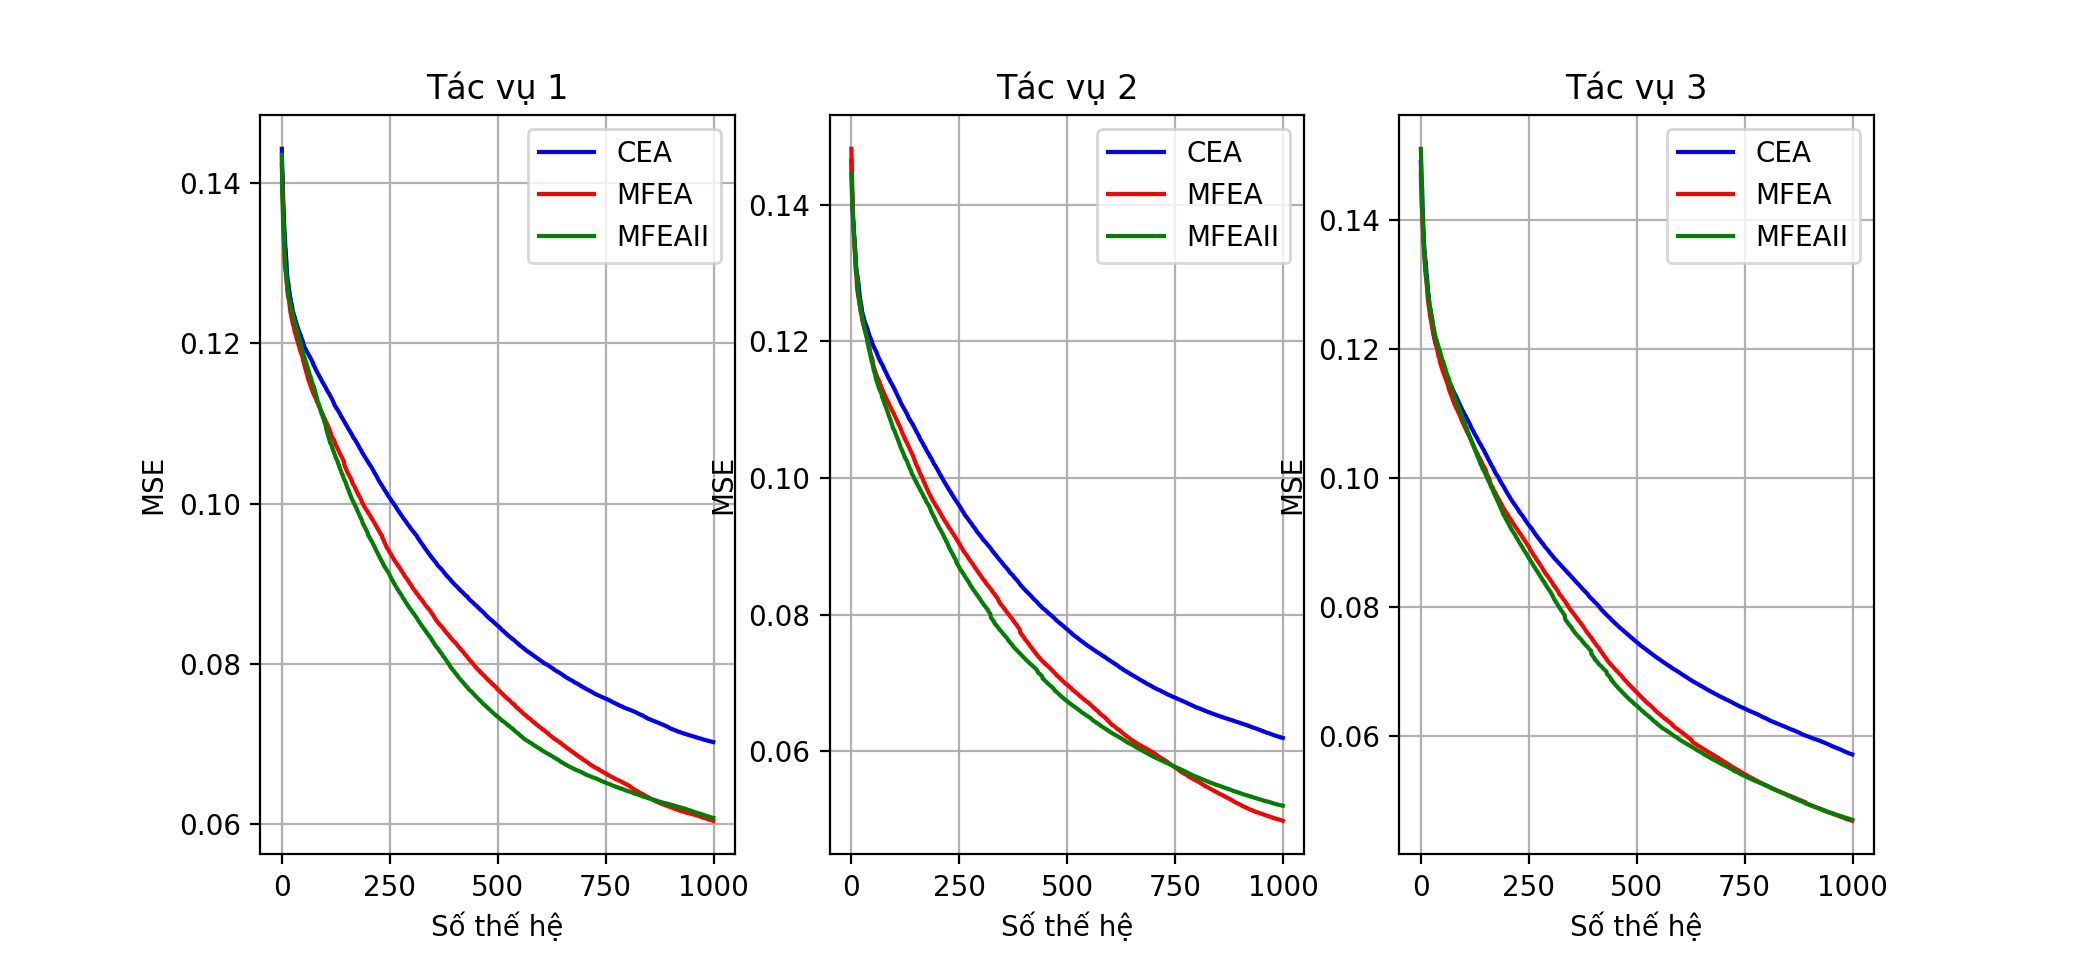
\includegraphics[width=\textwidth,height=\textheight,keepaspectratio]{thesis/images/results/nbit_1layer/6bit1_task.png}}
    \scalebox{.7}{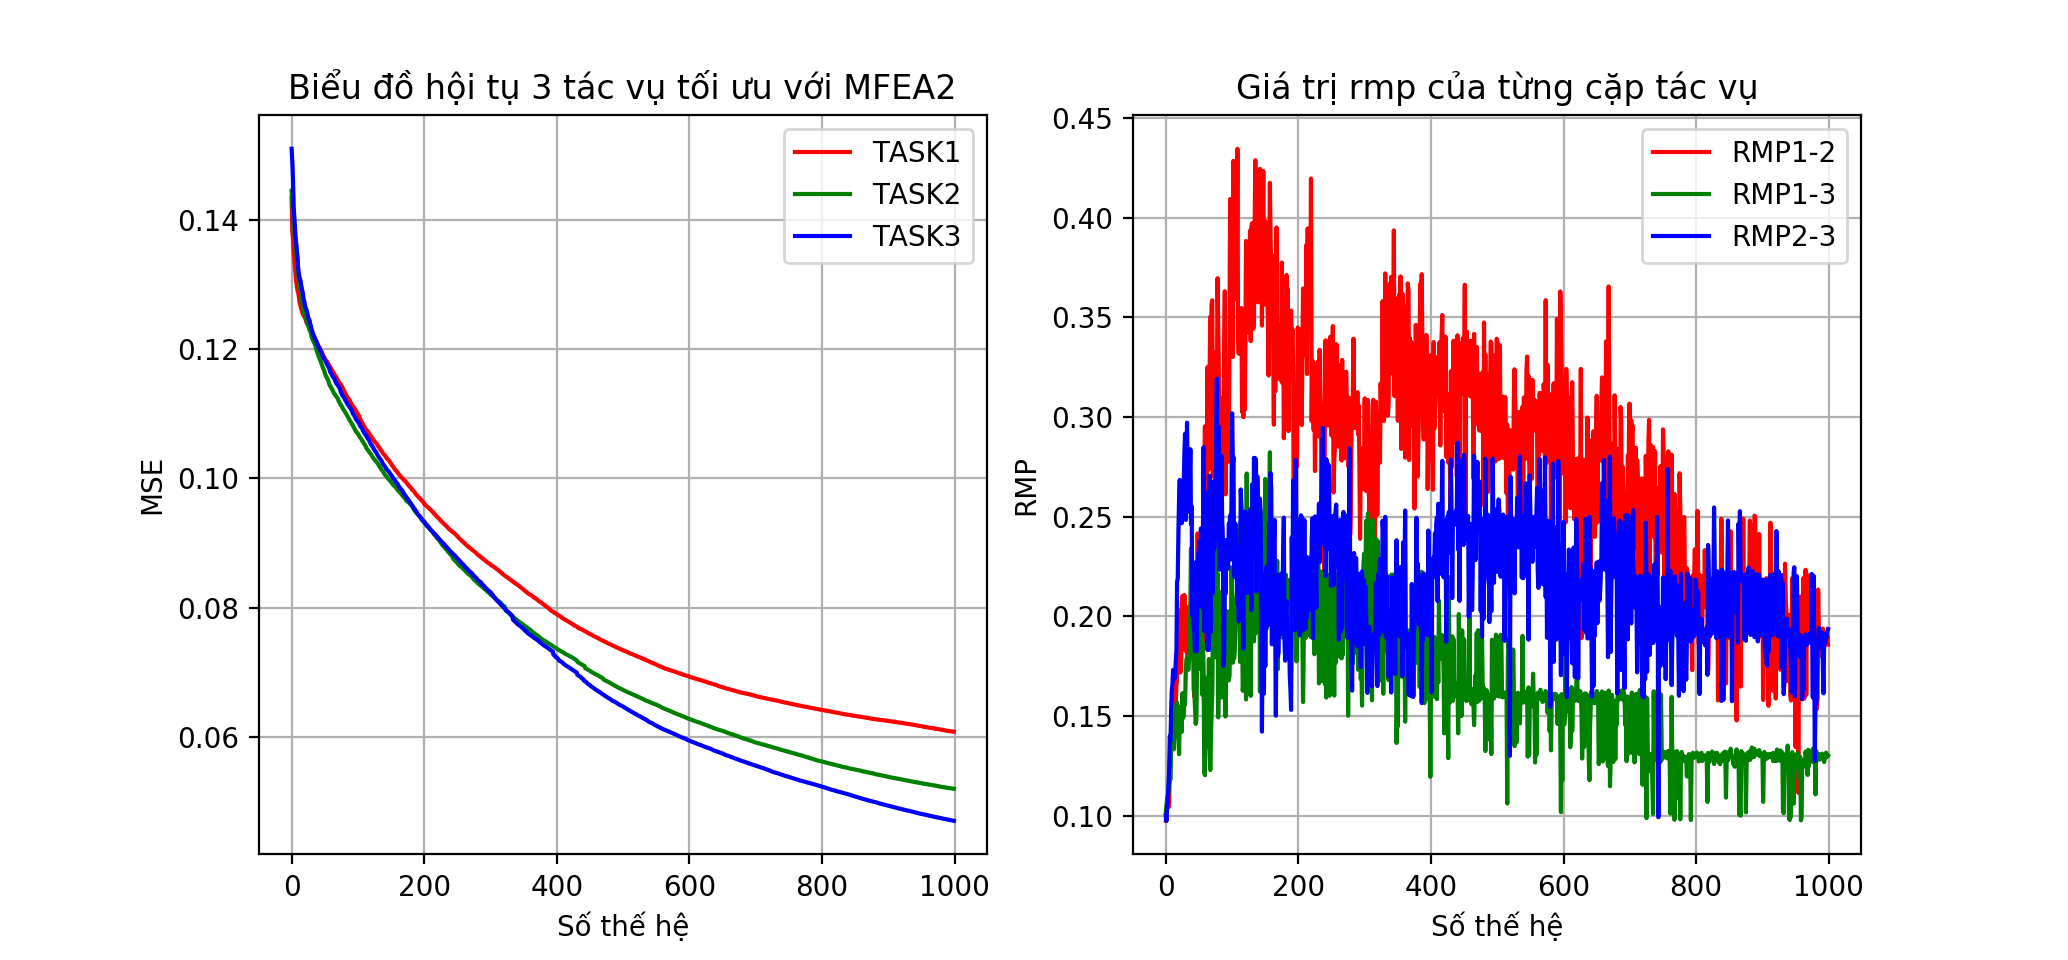
\includegraphics[width=\textwidth,height=\textheight,keepaspectratio]{thesis/images/results/nbit_1layer/6bit1_rmp.png}}
    \label{fig:6bit_1}
    \caption{Bài 6bit(5,6,7): Biểu đồ hội tụ của từng tác vụ trên các thuật toán và biểu đồ phân tích MFEA-II theo giá trị rmp}

\end{figure}
\begin{figure}[H]

    \centering
    \scalebox{.7}{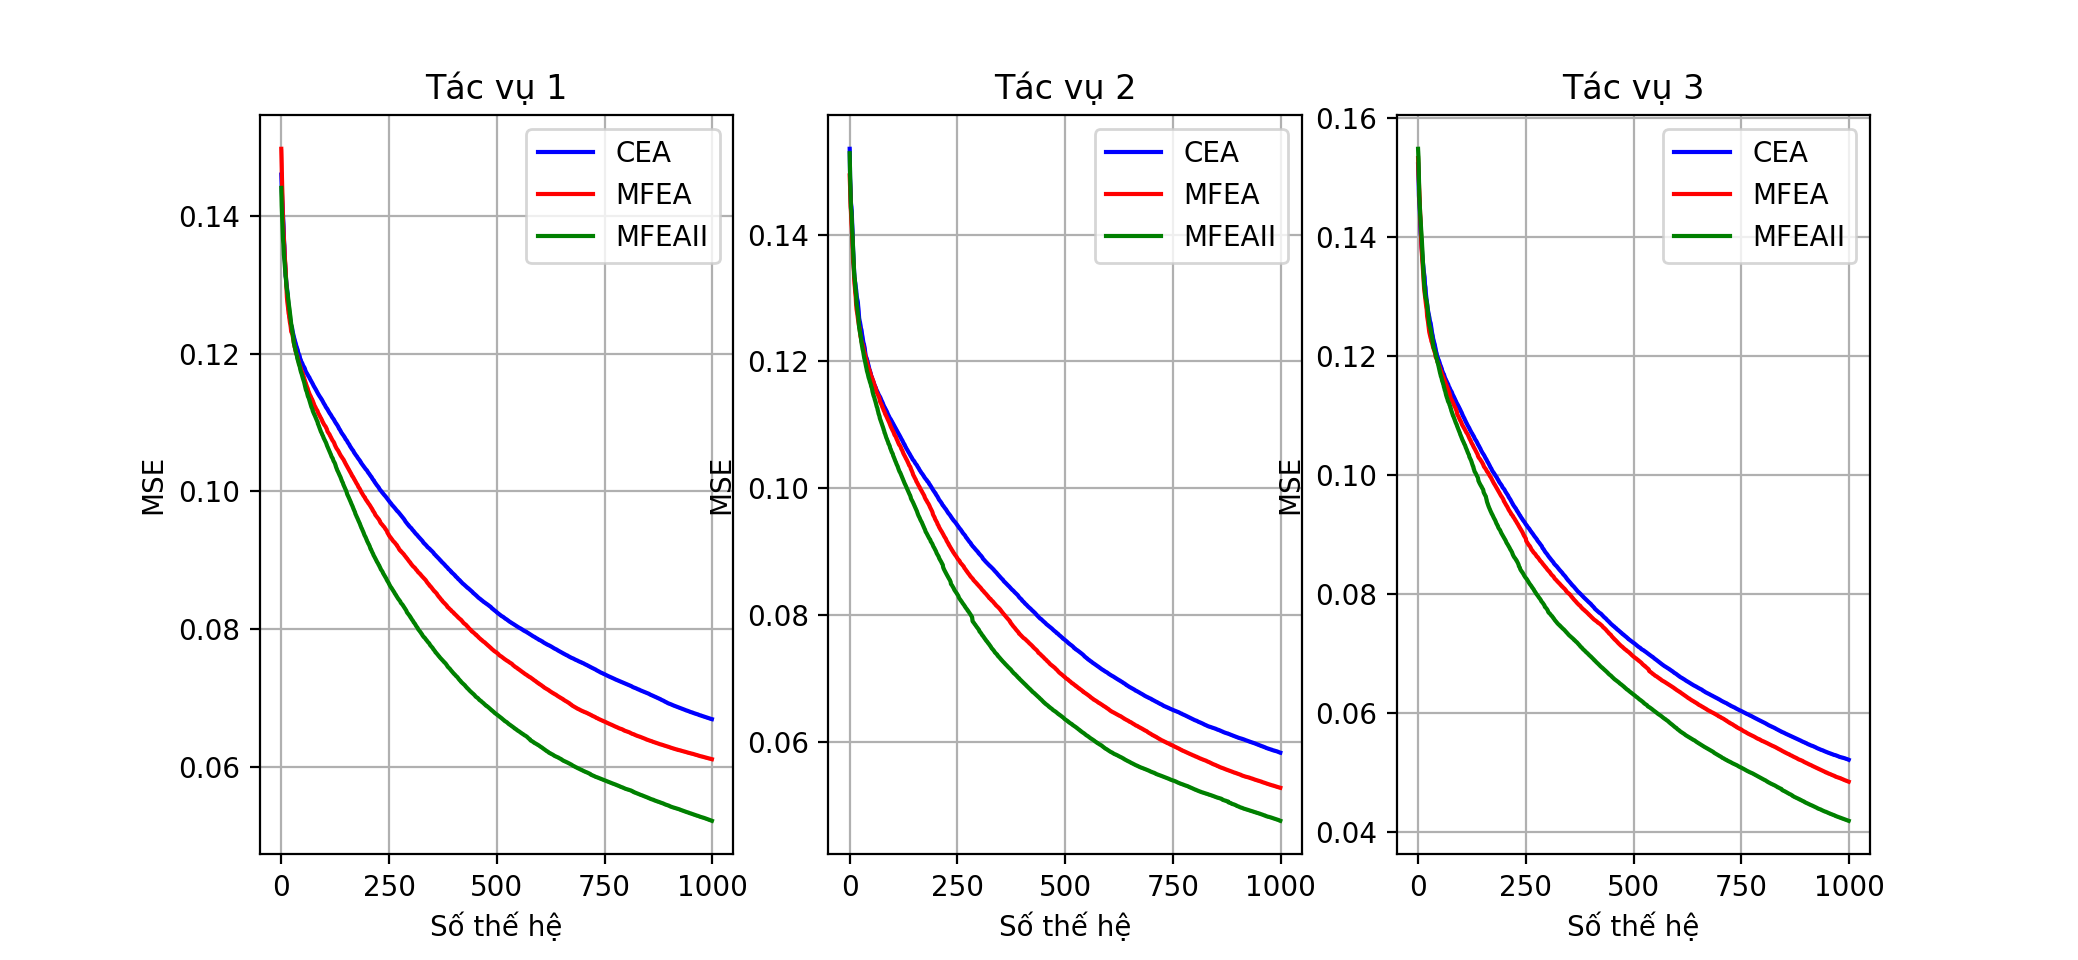
\includegraphics[width=\textwidth,height=\textheight,keepaspectratio]{thesis/images/results/nbit_1layer/6bit2_task.png}}
    \scalebox{.7}{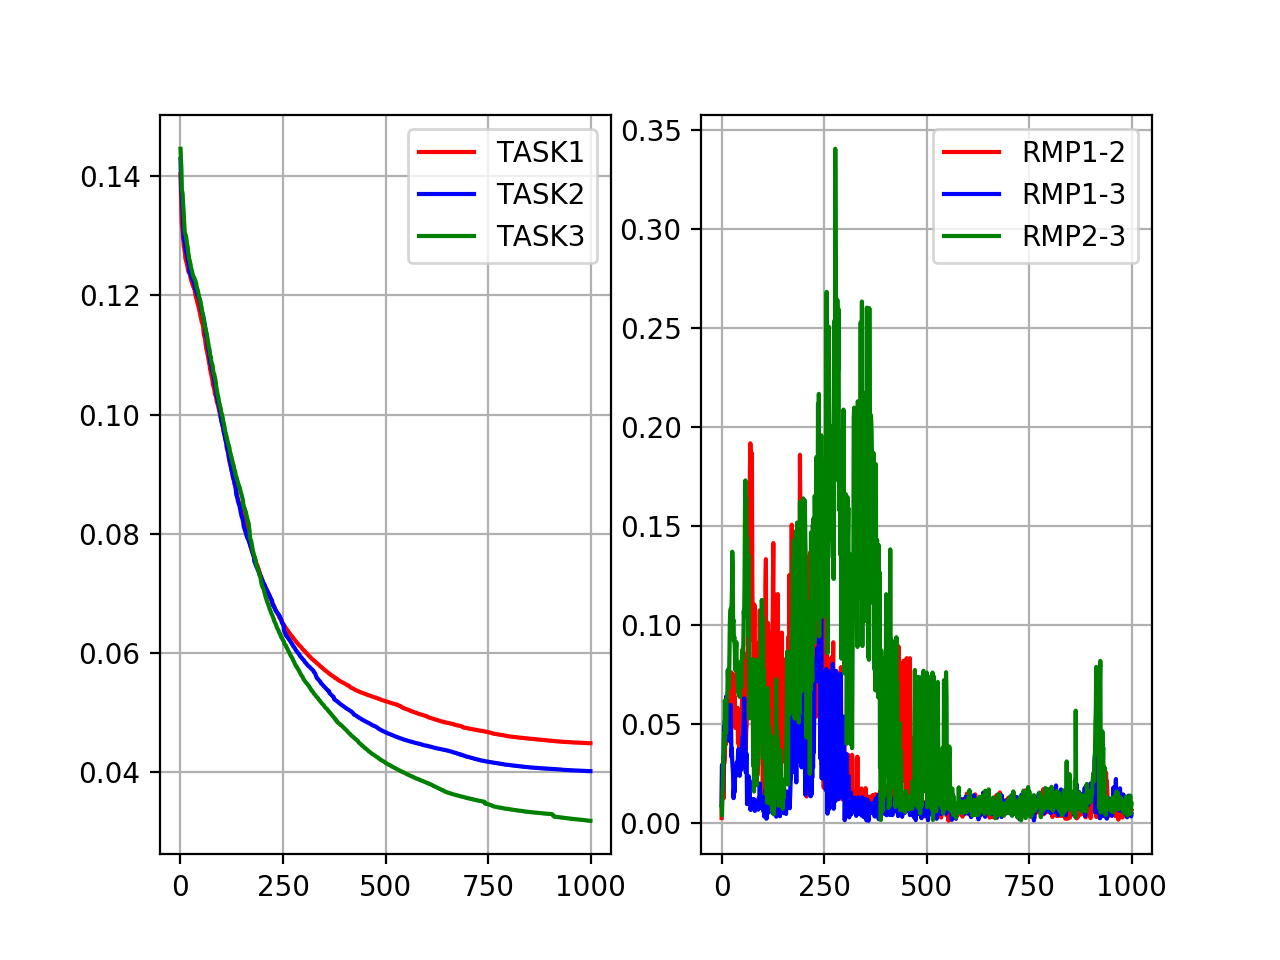
\includegraphics[width=\textwidth,height=\textheight,keepaspectratio]{thesis/images/results/nbit_1layer/6bit2_rmp.png}}
    \label{fig:6bit2_1layer}
        \caption{Bài 6bit(6,7,8): Biểu đồ hội tụ của từng tác vụ trên các thuật toán và biểu đồ phân tích MFEA-II theo giá trị rmp}

\end{figure}
\begin{figure}[H]
    \centering

    \scalebox{.7}{\includegraphics[width=\textwidth,height=\textheight,keepaspectratio]{thesis/images/results/nbit_1layer/8bit1_task.png}}
    \scalebox{.7}{\includegraphics[width=\textwidth,height=\textheight,keepaspectratio]{thesis/images/results/nbit_1layer/8bit1_rmp.png}}
    \label{fig:8bit1_1layer}
    \caption{Bài 8bit(5,6,7):Biểu đồ hội tụ của từng tác vụ trên các thuật toán và biểu đồ phân tích MFEA-II theo giá trị rmp}

\end{figure}
\begin{figure}[H]
    \centering

    \scalebox{.7}{\includegraphics[width=\textwidth,height=\textheight,keepaspectratio]{thesis/images/results/nbit_1layer/8bit2_task.png}}
    \scalebox{.7}{\includegraphics[width=\textwidth,height=\textheight,keepaspectratio]{thesis/images/results/nbit_1layer/8bit2_rmp.png}}
    \label{fig:8bit2_1layer}
    \caption{Bài 8bit(6,7,8): Biểu đồ hội tụ của từng tác vụ trên các thuật toán và biểu đồ phân tích MFEA-II theo giá trị rmp}

\end{figure}

\subsubsection{Bảng kết quả thực nghiệm - mạng neural cùng độ sâu 2 lớp ẩn}
\begin{table} [H]
    \begin{center}
    \caption{Kết quả thực nghiệm huấn luyện ANN 2 lớp ẩn}
    \begin{tabular}{|c|c|c|c|c|}
    \hline
    \multirow{1}{*}{\textbf{Bài toán}} &
    \multirow{1}{*}{\textbf{Method}} & \multicolumn{1}{c|}{\textbf{Tác vụ 1}} & \multicolumn{1}{c|}{\textbf{Tác vụ 2}} & \multicolumn{1}{c|}{\textbf{Tác vụ 3}} \\ \hline
    \multirow{3}{*} 
    {8-bit} &
    CEA & $0.075 \pm 0.012865$ & $0.0713 \pm 0.013116$ & $0.0718 \pm 0.012432$  \\
    & MFEA-I & $0.0738 \pm 0.012508$ & $0.0684 \pm 0.013252$ & $0.0669 \pm 0.015076$   \\
    & MFEA-II & $\mathbf{0.0705 \pm 0.012856}$ & $\mathbf{0.0624 \pm 0.011079}$ & $\mathbf{0.0595 \pm 0.011252}$\\\hline
    \multirow{3}{*} 
    {9-bit} &
    CEA & $0.0826 \pm 0.010588$ & $0.0751 \pm 0.014406$ & $0.0785 \pm 0.010766$  \\
    & MFEA-I & $0.0827 \pm 0.010438$ & $0.0762 \pm 0.009495$ & $0.0737 \pm 0.009766$ \\
    & MFEA-II & $\mathbf{0.0795 \pm 0.012865}$ & $\mathbf{0.0705 \pm 0.009581}$ & $\mathbf{0.0685 \pm 0.011156}$ \\\hline
    \multirow{3}{*} 
    {10-bit} &
    CEA & $0.0853 \pm 0.01105$ & $0.0862 \pm 0.008326$ & $0.0856 \pm 0.008919$  \\
    & MFEA-I  & $0.0855 \pm 0.012229$ & $\mathbf{0.0782 \pm 0.009659}$ & $\mathbf{0.0752 \pm 0.009681}$ \\
    & MFEA-II & $\mathbf{0.0833 \pm 0.010222}$ & $0.0791 \pm 0.009846$ & $0.0762 \pm 0.010419$ \\\hline
    \end{tabular}
    \end{center}

    \label{tab:result:nbit}
\end{table}

\subsubsection{Biểu đồ hội tụ - Mạng neural cùng độ sâu 2 lớp ẩn}
\begin{figure}[h!]
    \centering
    \scalebox{.7}{\includegraphics[width=\textwidth,height=\textheight,keepaspectratio]{thesis/images/results/nbit_2layer/8bit1_task.png}}
    \scalebox{.7}{\includegraphics[width=\textwidth,height=\textheight,keepaspectratio]{thesis/images/results/nbit_2layer/8bit1_rmp.png}}
    \caption{Bài 8bit: Biểu đồ hội tụ của từng tác vụ trên các thuật toán và biểu đồ phân tích MFEA-II theo giá trị rmp}
    \label{fig:8bit_2layer}
\end{figure}
\begin{figure}[h!]
    \centering
    \scalebox{.7}{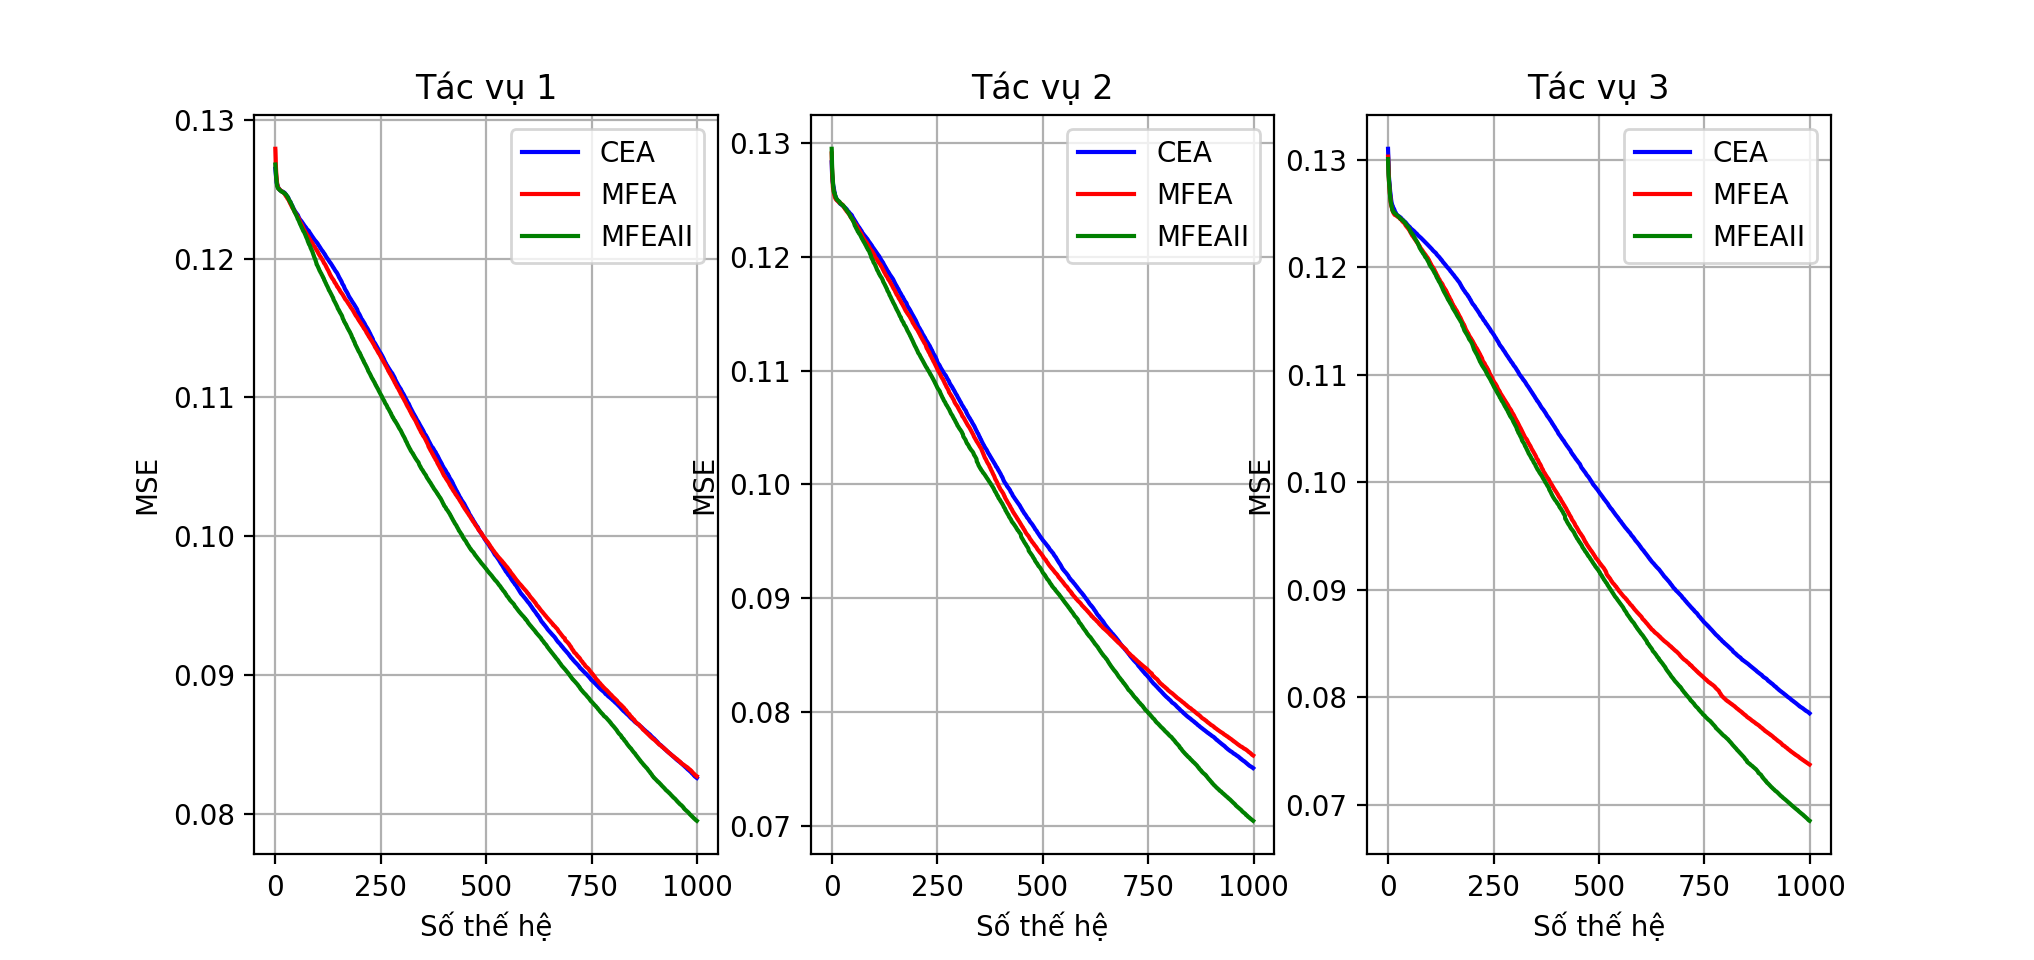
\includegraphics[width=\textwidth,height=\textheight,keepaspectratio]{thesis/images/results/nbit_2layer/9bit1_task.png}}
    \scalebox{.7}{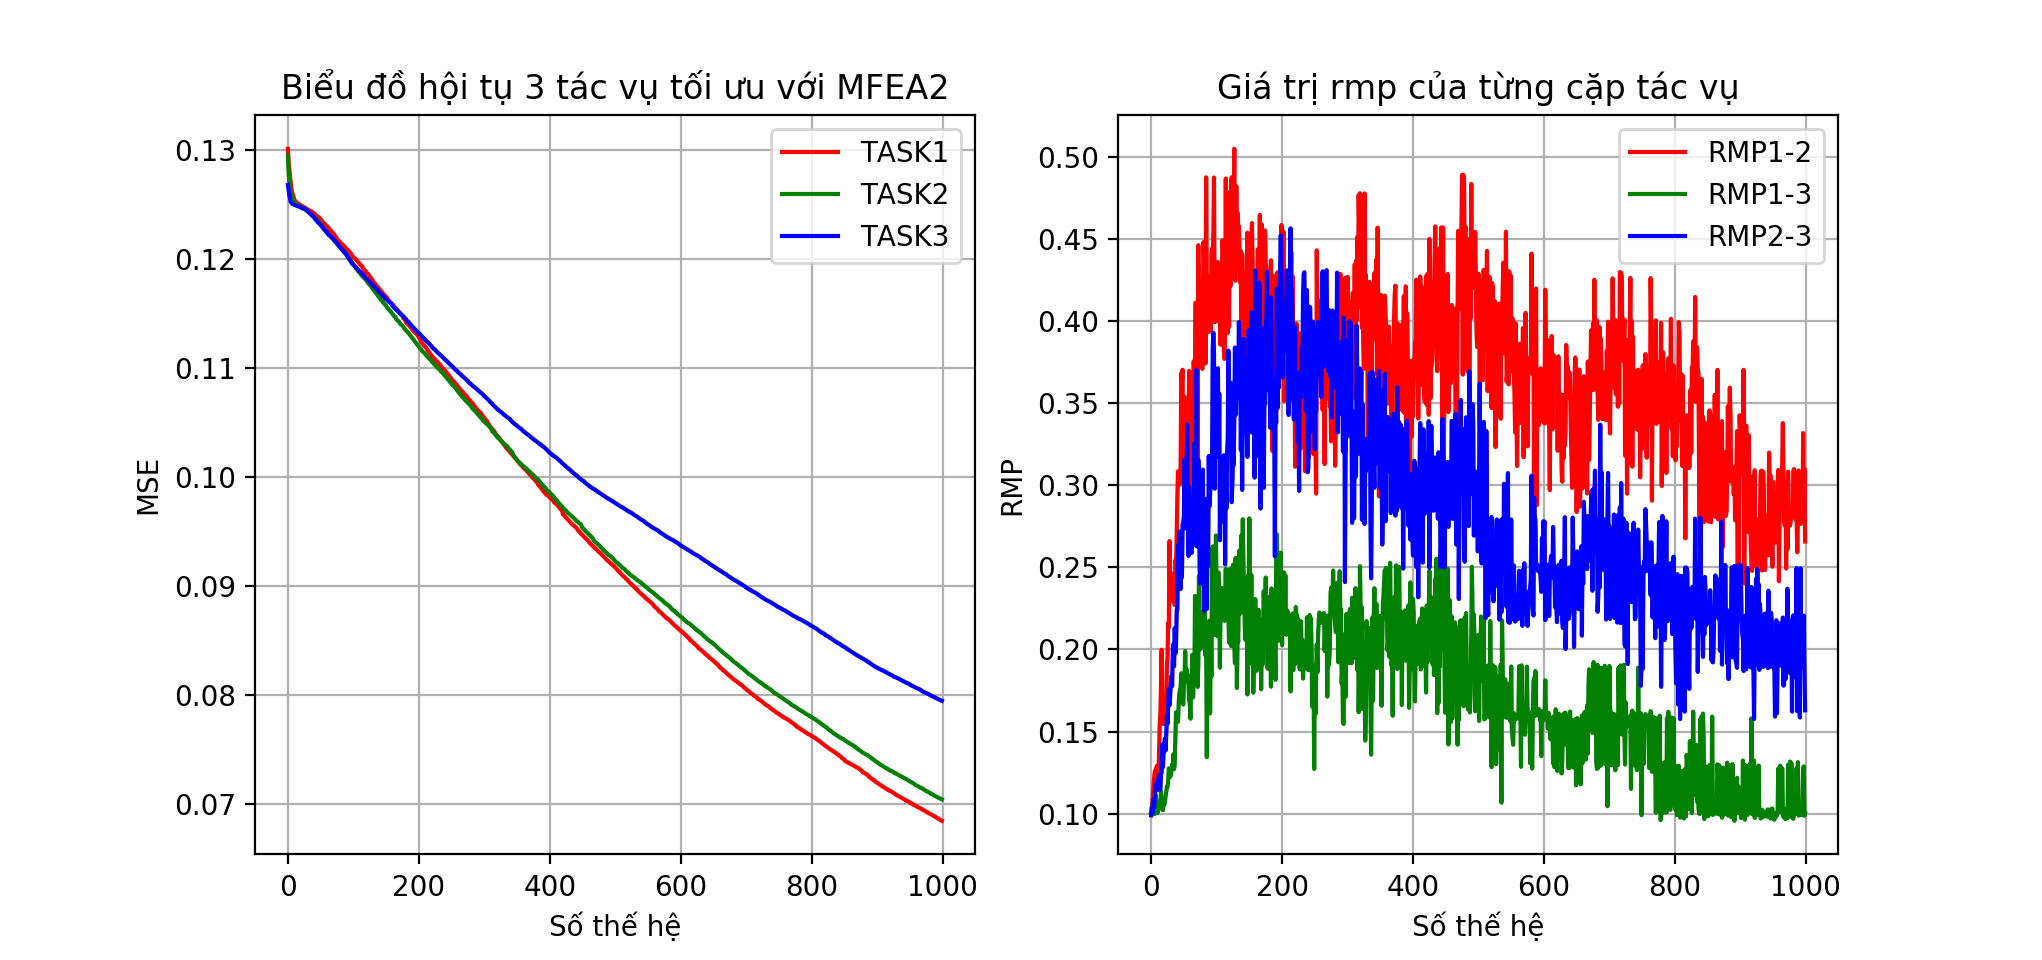
\includegraphics[width=\textwidth,height=\textheight,keepaspectratio]{thesis/images/results/nbit_2layer/9bit1_rmp.png}}
    \caption{Bài 9bit: Biểu đồ hội tụ của từng tác vụ trên các thuật toán và biểu đồ phân tích MFEA-II theo giá trị rmp}
    \label{fig:9bit_2layer}
\end{figure}
\begin{figure}[h!]
    \centering
    \scalebox{.7}{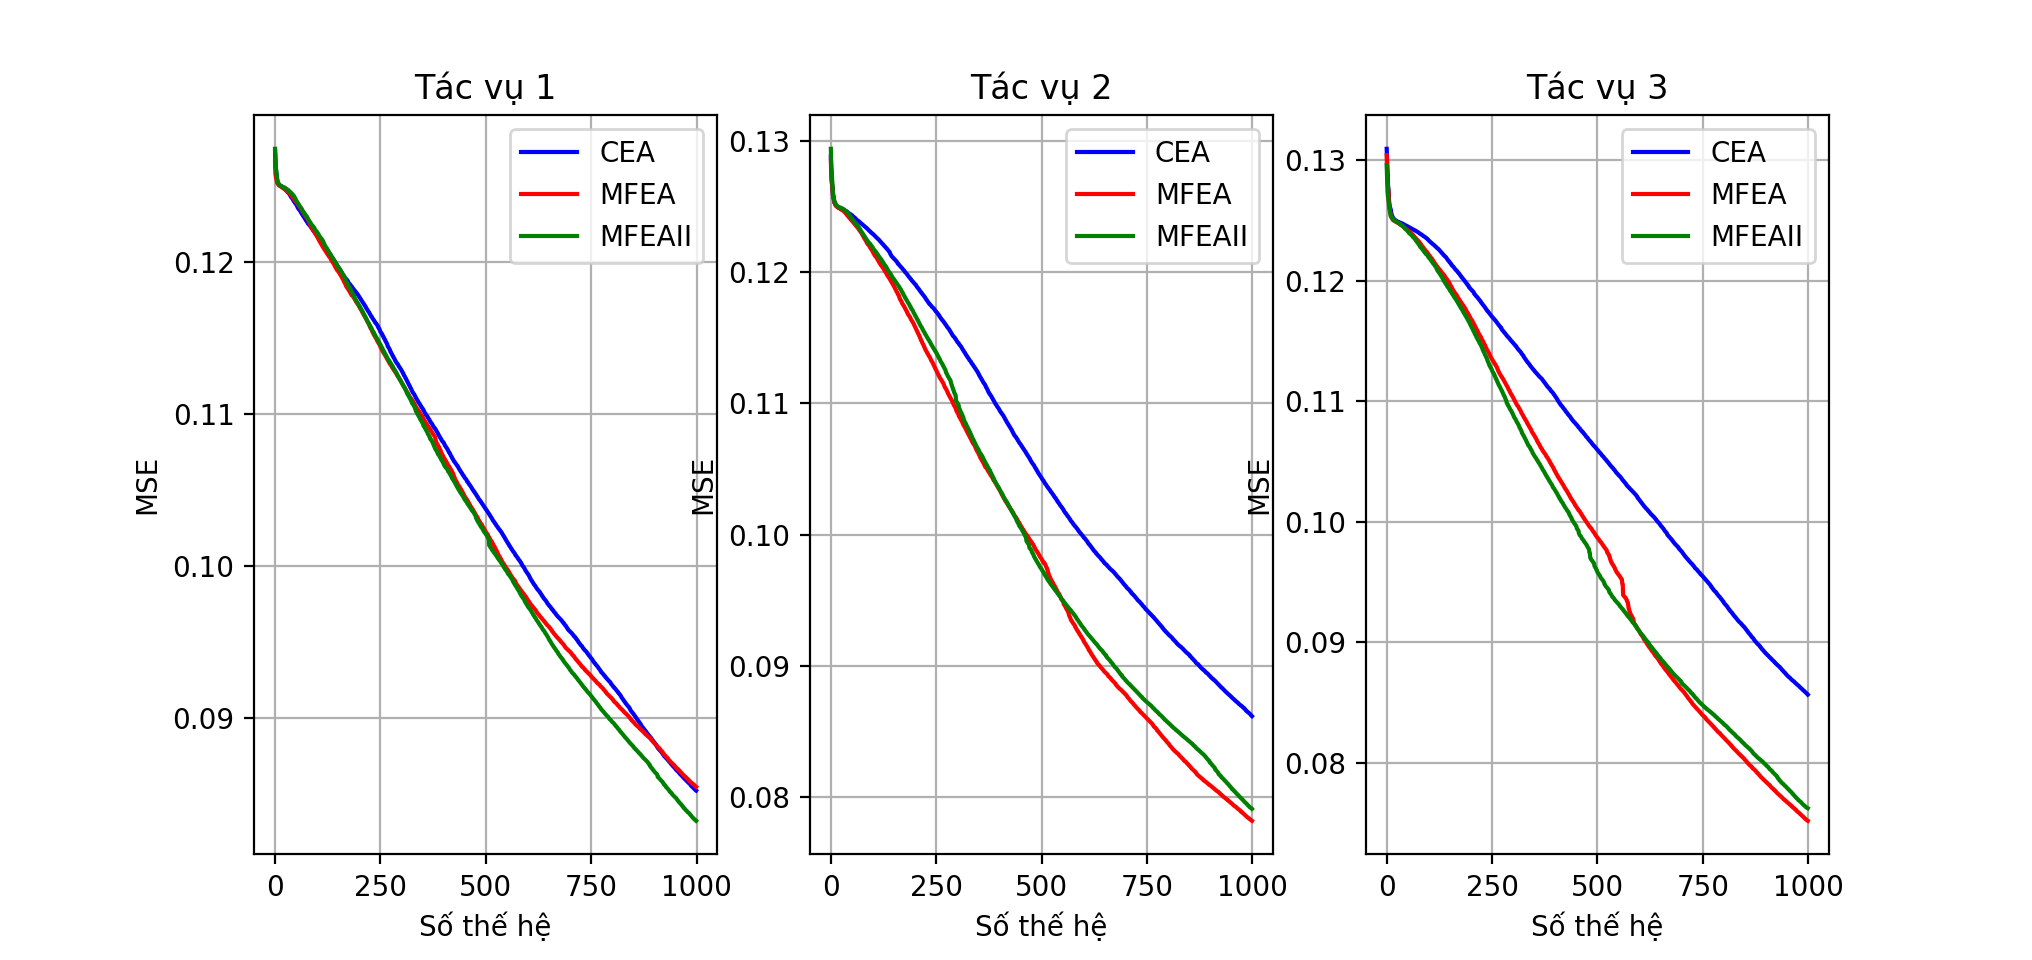
\includegraphics[width=\textwidth,height=\textheight,keepaspectratio]{thesis/images/results/nbit_2layer/10bit1_task.png}}
    \scalebox{.7}{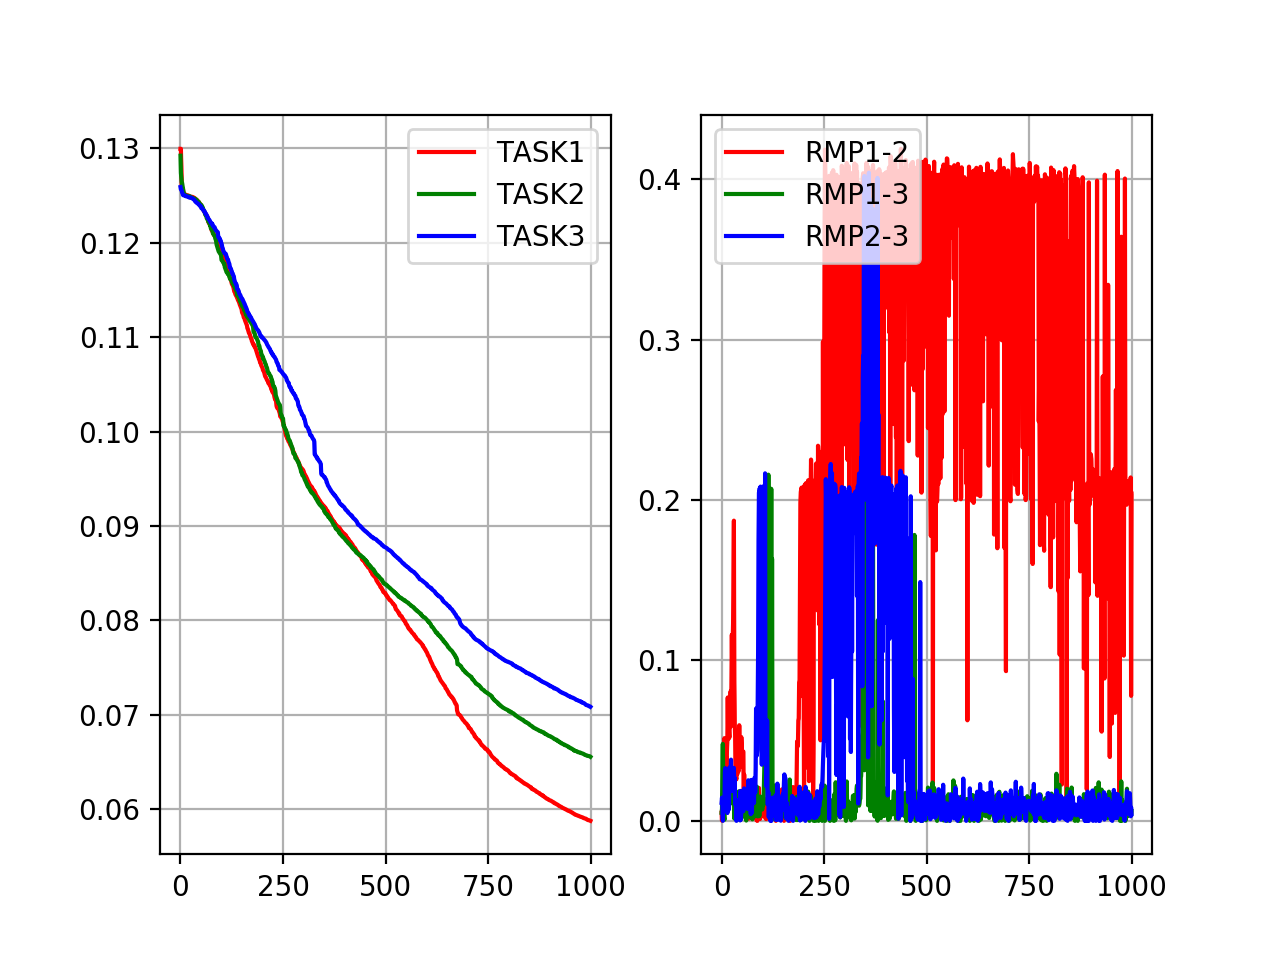
\includegraphics[width=\textwidth,height=\textheight,keepaspectratio]{thesis/images/results/nbit_2layer/10bit1_rmp.png}}
    \caption{Bài 10bit: Biểu đồ hội tụ của từng tác vụ trên các thuật toán và biểu đồ phân tích MFEA-II theo giá trị rmp}
    \label{fig:10bit_2layer}
\end{figure}
\newpage

\subsubsection{Bảng kết quả thực nghiệm - mạng neural khác độ sâu}
\begin{table} [H]
    \begin{center}
    \caption{Kết quả huấn luyện ANN khác độ sâu}
    \begin{tabular}{|c|c|c|c|c|}
    \hline
    \multirow{1}{*}{\textbf{Bài toán}} &
    \multirow{1}{*}{\textbf{Method}} & \multicolumn{1}{c|}{\textbf{Tác vụ 1}} & \multicolumn{1}{c|}{\textbf{Tác vụ 2}} & \multicolumn{1}{c|}{\textbf{Tác vụ 3}} \\ \hline
    \multirow{3}{*} 
    {8-bit} &
    CEA & $0.0789 \pm 0.0172$ & $0.0815 \pm 0.0136$ & $\mathbf{0.0794 \pm 0.0156}$ \\
    & MFEA-I & $0.0778 \pm 0.0153$ & $0.0805 \pm 0.0142$ & $0.0814 \pm 0.0119$  \\
    & MFEA-II & $\mathbf{0.0721} \pm 0.0148$ & $\mathbf{0.0759 \pm 0.015}$ & $0.0822 \pm 0.0143$\\\hline
    \multirow{3}{*} 
    {9-bit} &
    CEA & $0.0843 \pm 0.0154$ & $0.0869 \pm 0.0141$ & $0.086 \pm 0.0128$  \\
    & MFEA-I & $0.0844 \pm 0.0124$ & $\mathbf{0.0795 \pm 0.0144}$ & $\mathbf{0.081 \pm 0.0134}$ \\
    & MFEA-II & $\mathbf{0.0828 \pm 0.0129}$ & $0.0818 \pm 0.0131$ & $0.0864 \pm 0.0147$ \\\hline
    \multirow{3}{*} 
    {10-bit} &
    CEA & $0.089 \pm 0.0131$ & $0.0922 \pm 0.0164$ & $0.0928 \pm 0.0124$  \\
    & MFEA-I  & $0.0879 \pm 0.0091$ & $0.0888 \pm 0.0124$ & $\mathbf{0.0873 \pm 0.0111}$ \\
    & MFEA-II & $\mathbf{0.0867 \pm 0.0079}$ & $\mathbf{0.0862 \pm 0.0103}$ & $0.0905 \pm 0.0104$ \\\hline
    \end{tabular}
    \end{center}
    \label{tab:result:nbit}

\end{table}

\subsubsection{Biểu đồ hội tụ - mạng neural khác độ sâu}

\begin{figure}[h!]
    \centering
    \scalebox{.57}{\includegraphics[width=\textwidth,height=\textheight,keepaspectratio]{thesis/images/results/multilayers/8bit2_task.png}}
    \scalebox{.57}{\includegraphics[width=\textwidth,height=\textheight,keepaspectratio]{thesis/images/results/multilayers/8bit2_rmp.png}}
    \caption{Bài 8bit: Biểu đồ hội tụ của từng tác vụ trên các thuật toán và biểu đồ phân tích MFEA-II theo giá trị rmp}
    \label{fig:8bit_multilayer}
\end{figure}
\begin{figure}[h!]
    \centering
    \scalebox{.6}{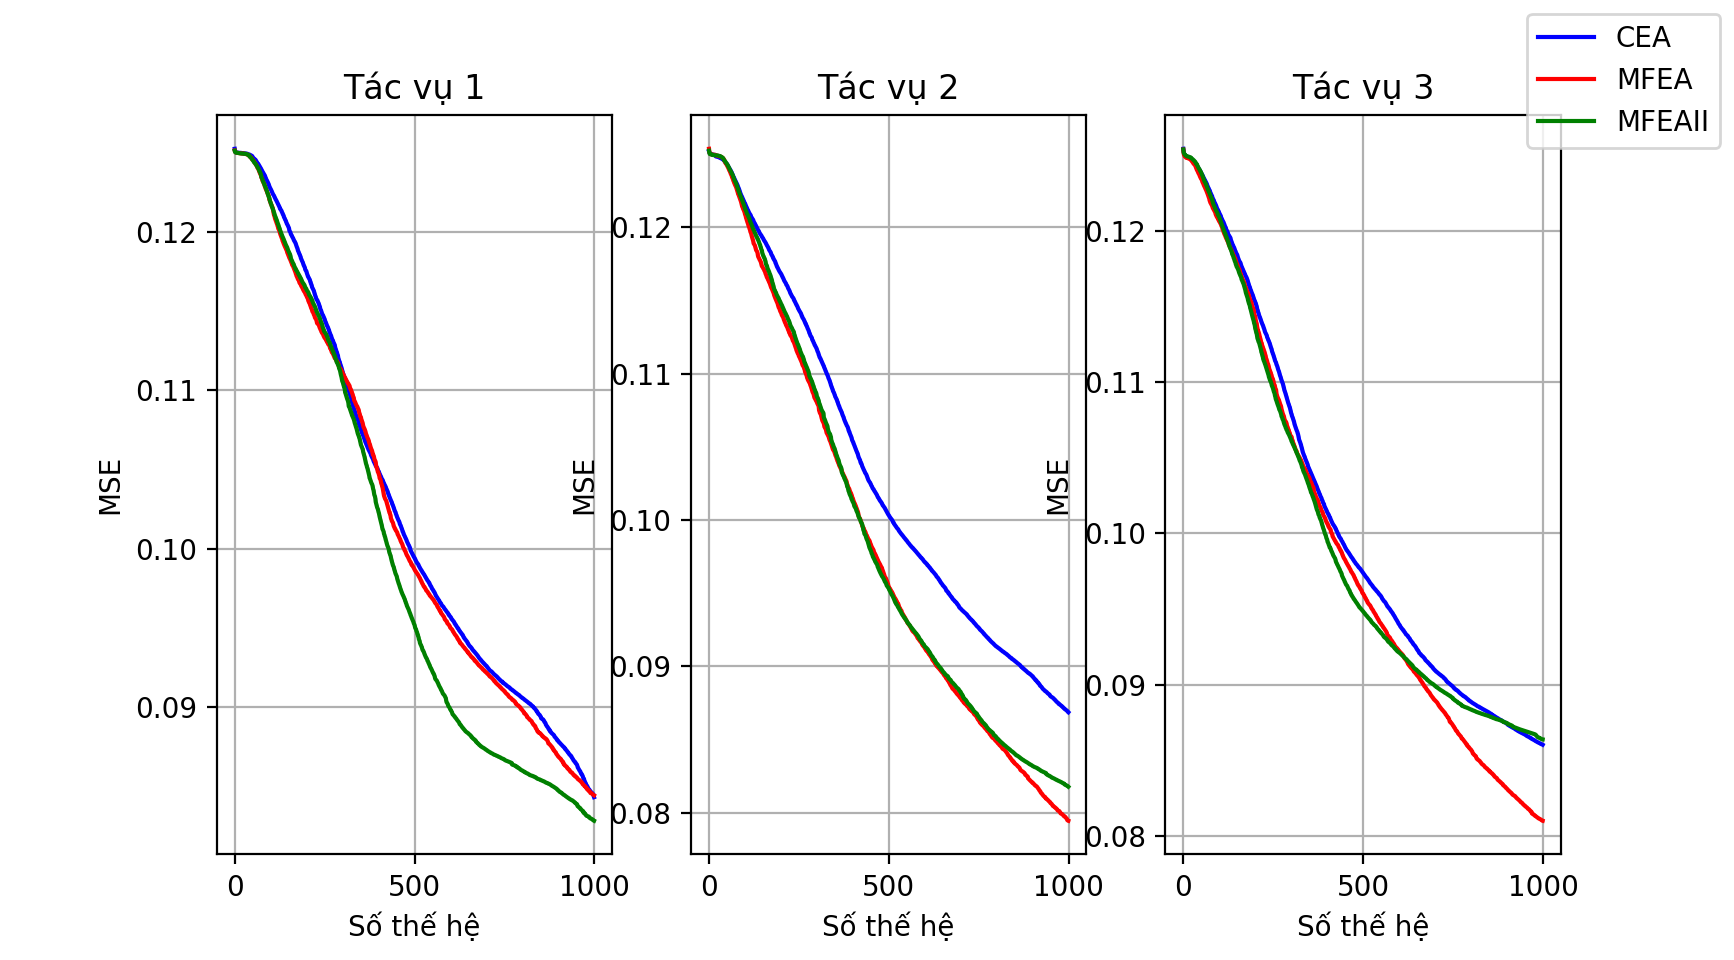
\includegraphics[width=\textwidth,height=\textheight,keepaspectratio]{thesis/images/results/multilayers/9bit2_task.png}}
    \scalebox{.6}{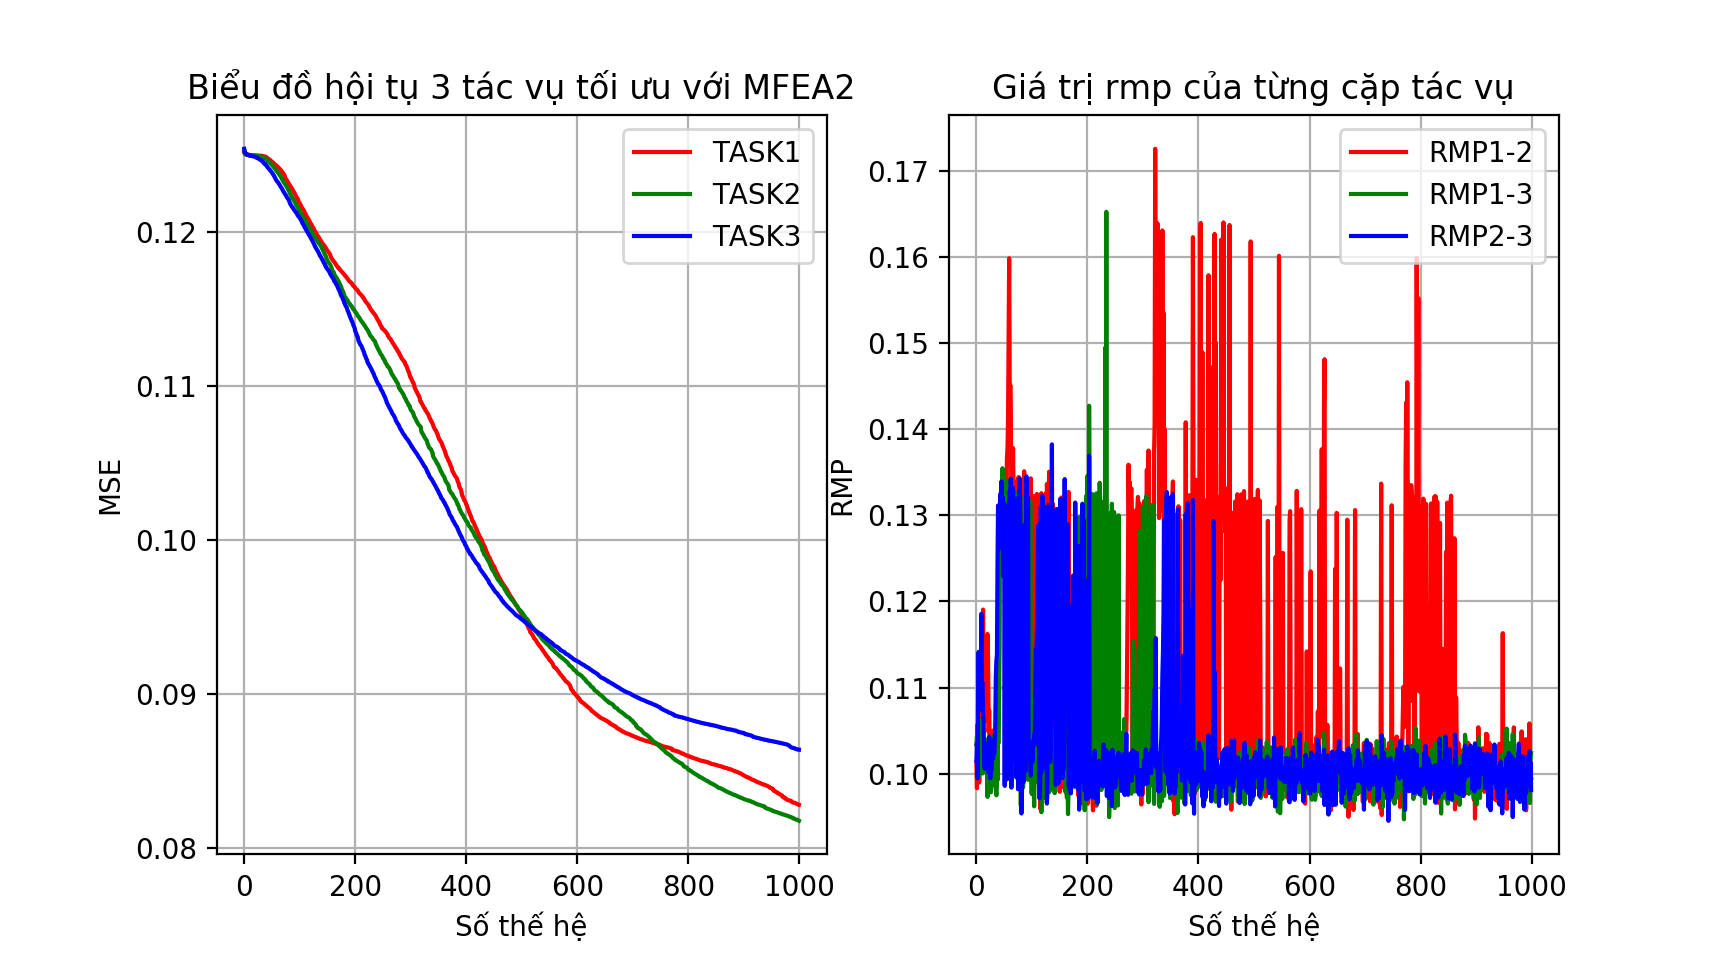
\includegraphics[width=\textwidth,height=\textheight,keepaspectratio]{thesis/images/results/multilayers/9bit2_rmp.png}}
    \caption{Bài 9bit: Biểu đồ hội tụ của từng tác vụ trên các thuật toán và biểu đồ phân tích MFEA-II theo giá trị rmp}
    \label{fig:8bit_multilayer}
\end{figure}
\begin{figure}[h!]
    \centering
    \scalebox{.5}{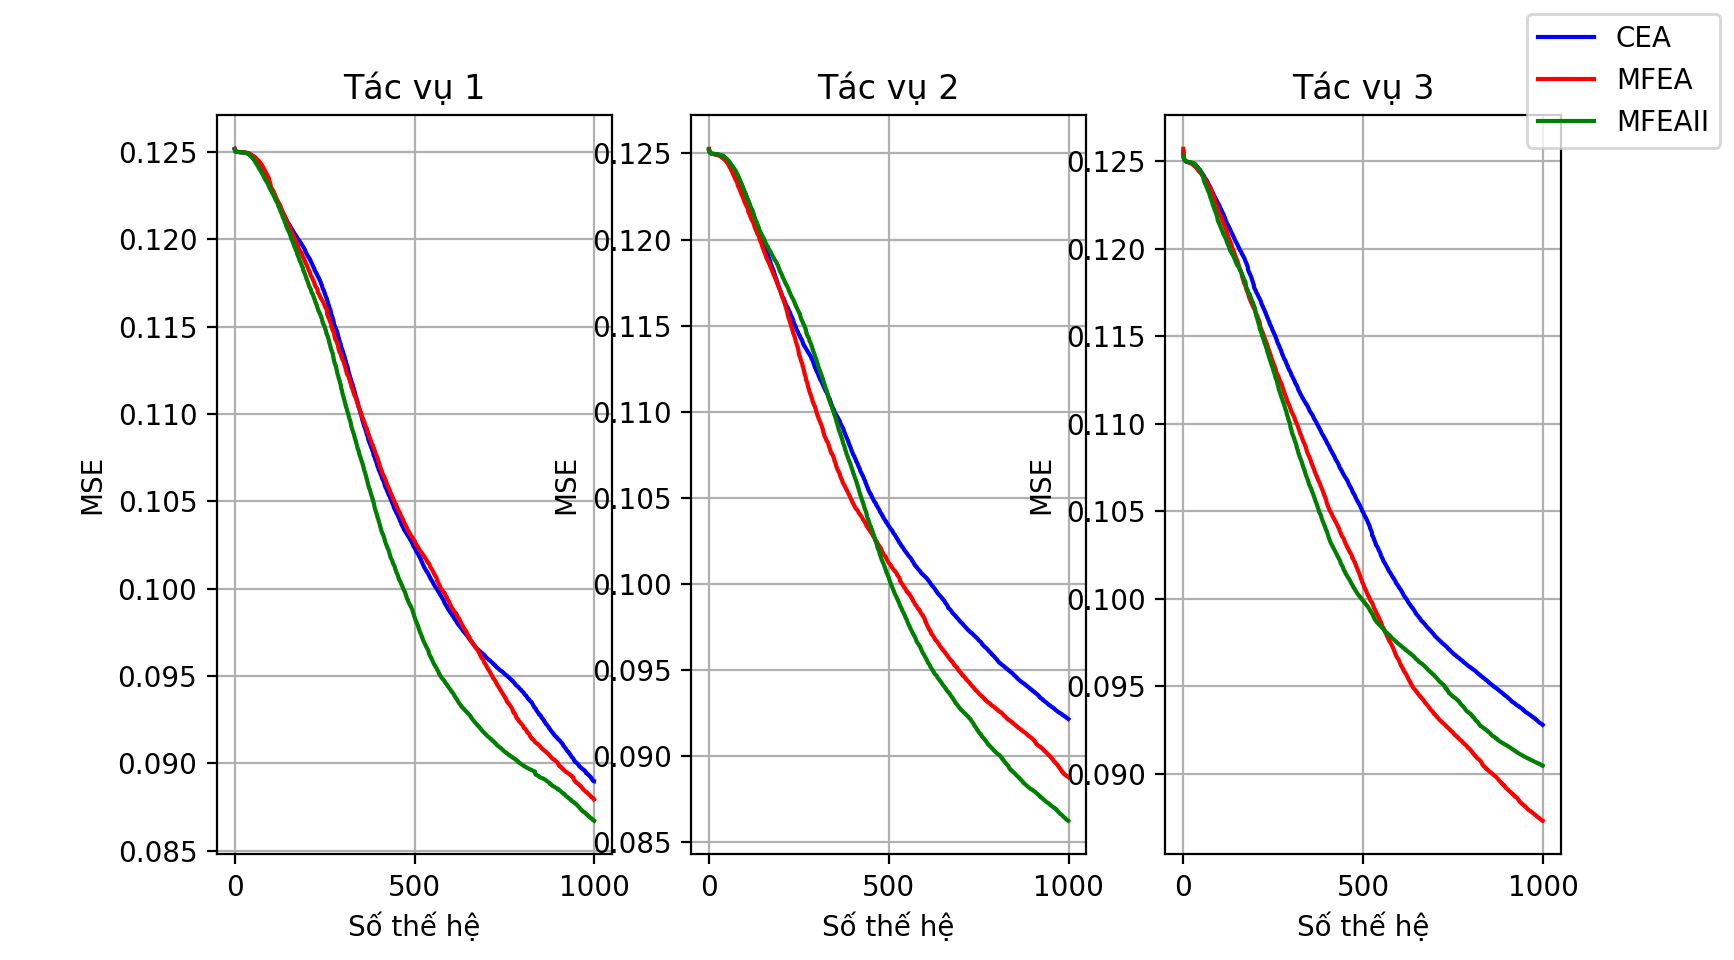
\includegraphics[width=\textwidth,height=\textheight,keepaspectratio]{thesis/images/results/multilayers/10bit2_task.png}}
    \scalebox{.5}{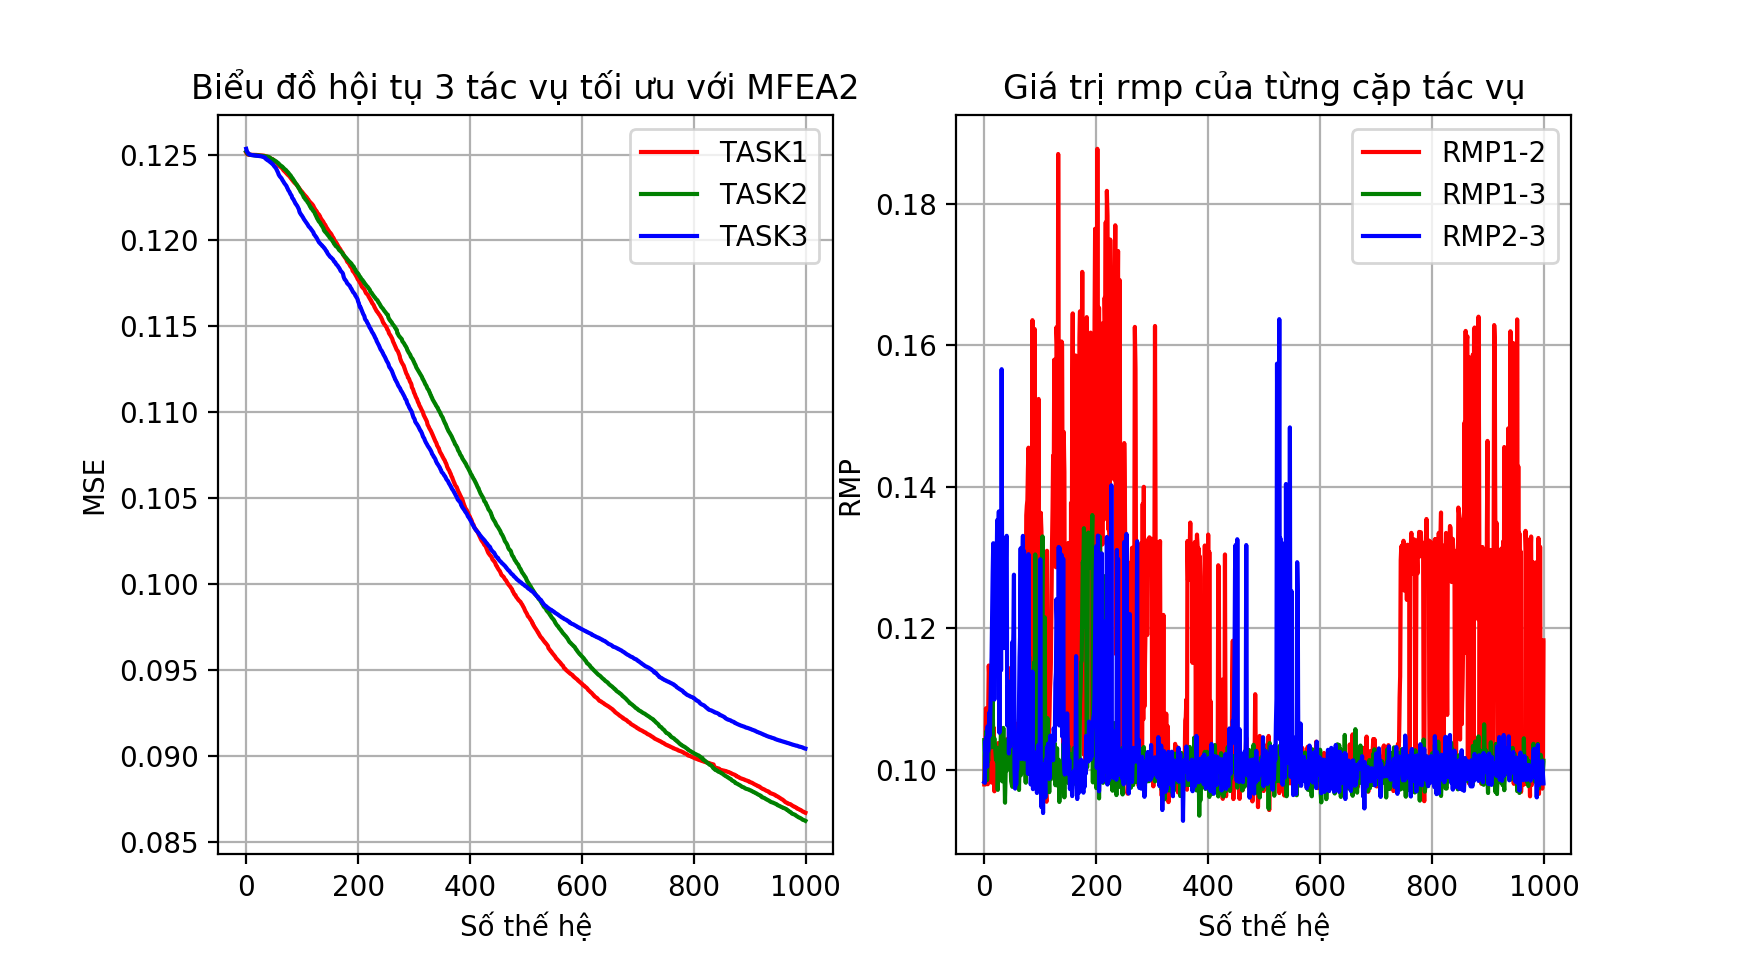
\includegraphics[width=\textwidth,height=\textheight,keepaspectratio]{thesis/images/results/multilayers/10bit2_rmp.png}}
    \caption{Bài 10bit: Biểu đồ hội tụ của từng tác vụ trên các thuật toán và biểu đồ phân tích MFEA-II theo giá trị rmp}
    \label{fig:8bit_multilayer}
\end{figure}

\subsubsection{Bảng kết quả thực nghiệm - bộ dữ liệu UCI với mạng neural cùng độ sâu}
\begin{table}[h!]
    \caption{Kết quả huấn luyện nhiều ANN trên bộ dữ liệu UCI cùng độ sâu}

    \begin{tabular}{|c|c|c|c|c|}
    \hline
    \multirow{1}{*}{\textbf{Instance}} & \multicolumn{1}{c|} {\textbf{Method}} & \multicolumn{1}{c|}{\textbf{Subtask1}} & \multicolumn{1}{c|}{\textbf{Subtask 2}} & \multicolumn{1}{c|}{\textbf{Subtask 3}} \\ \hline
    \multirow{3}{*} 
    {breastCancer} & CEA & $0.0097 \pm 0.0012$ & $0.0092 \pm 0.0007$ & $0.0093 \pm 0.0009$ \\
     & MFEA-I & $0.0097 \pm 0.0006$ & $0.0093 \pm 0.0005$ & $0.0091 \pm 0.0005$ \\ 
    & MFEA II & $\mathbf{0.0094 \pm 0.0008}$ & $\mathbf{0.0089 \pm 0.0006}$ & $\mathbf{0.0087 \pm 0.0004}$ \\ \hline
    \multirow{3}{*} {creditScreening} & CEA & $0.0509 \pm 0.0033$ & $0.0514 \pm 0.0033$ & $0.0508 \pm 0.004$ \\
   & MFEA-I & $0.0504 \pm 0.0024$ & $0.0503 \pm 0.0025$ & $0.0513 \pm 0.0022$ \\ 
   & MFEA-II & $\mathbf{0.0492 \pm 0.0023}$ & $\mathbf{0.0489 \pm 0.002}$ & $\mathbf{0.0491 \pm 0.002}$ \\ \hline
    \multirow{3}{*} {ionosphere} & CEA & $0.0384 \pm 0.0072$ & $0.0389 \pm 0.0129$ & $0.035 \pm 0.0047$ \\
    &MFEA-I & $0.0367 \pm 0.0068$ & $0.0347 \pm 0.0075$ & $0.0351 \pm 0.0088$ \\
    &MFEA-II & $\mathbf{0.0343 \pm 0.0079}$ & $\mathbf{0.0322 \pm 0.0071}$ & $\mathbf{0.032 \pm 0.007}$ \\\hline
    \multirow{3}{*} {ticTacToe} & CEA & $0.089 \pm 0.0047$ & $0.0838 \pm 0.0054$ & $0.0869 \pm 0.0049$ \\
    &MFEA-I & $0.0845 \pm 0.0049$ & $0.0818 \pm 0.0047$ & $0.0824 \pm 0.0047$ \\
    &MFEA-II & $\mathbf{0.082 \pm 0.0048}$ & $\mathbf{0.0815 \pm 0.0046}$ & $\mathbf{0.0812 \pm 0.0043}$  \\\hline
    
    \end{tabular}

    \label{tab:result:nbit}
\end{table}
\subsubsection{Biểu đồ hội tụ - bộ dữ liệu UCI với mạng neural cùng độ sâu}

\begin{figure}[h!]
    \centering
    \scalebox{.7}{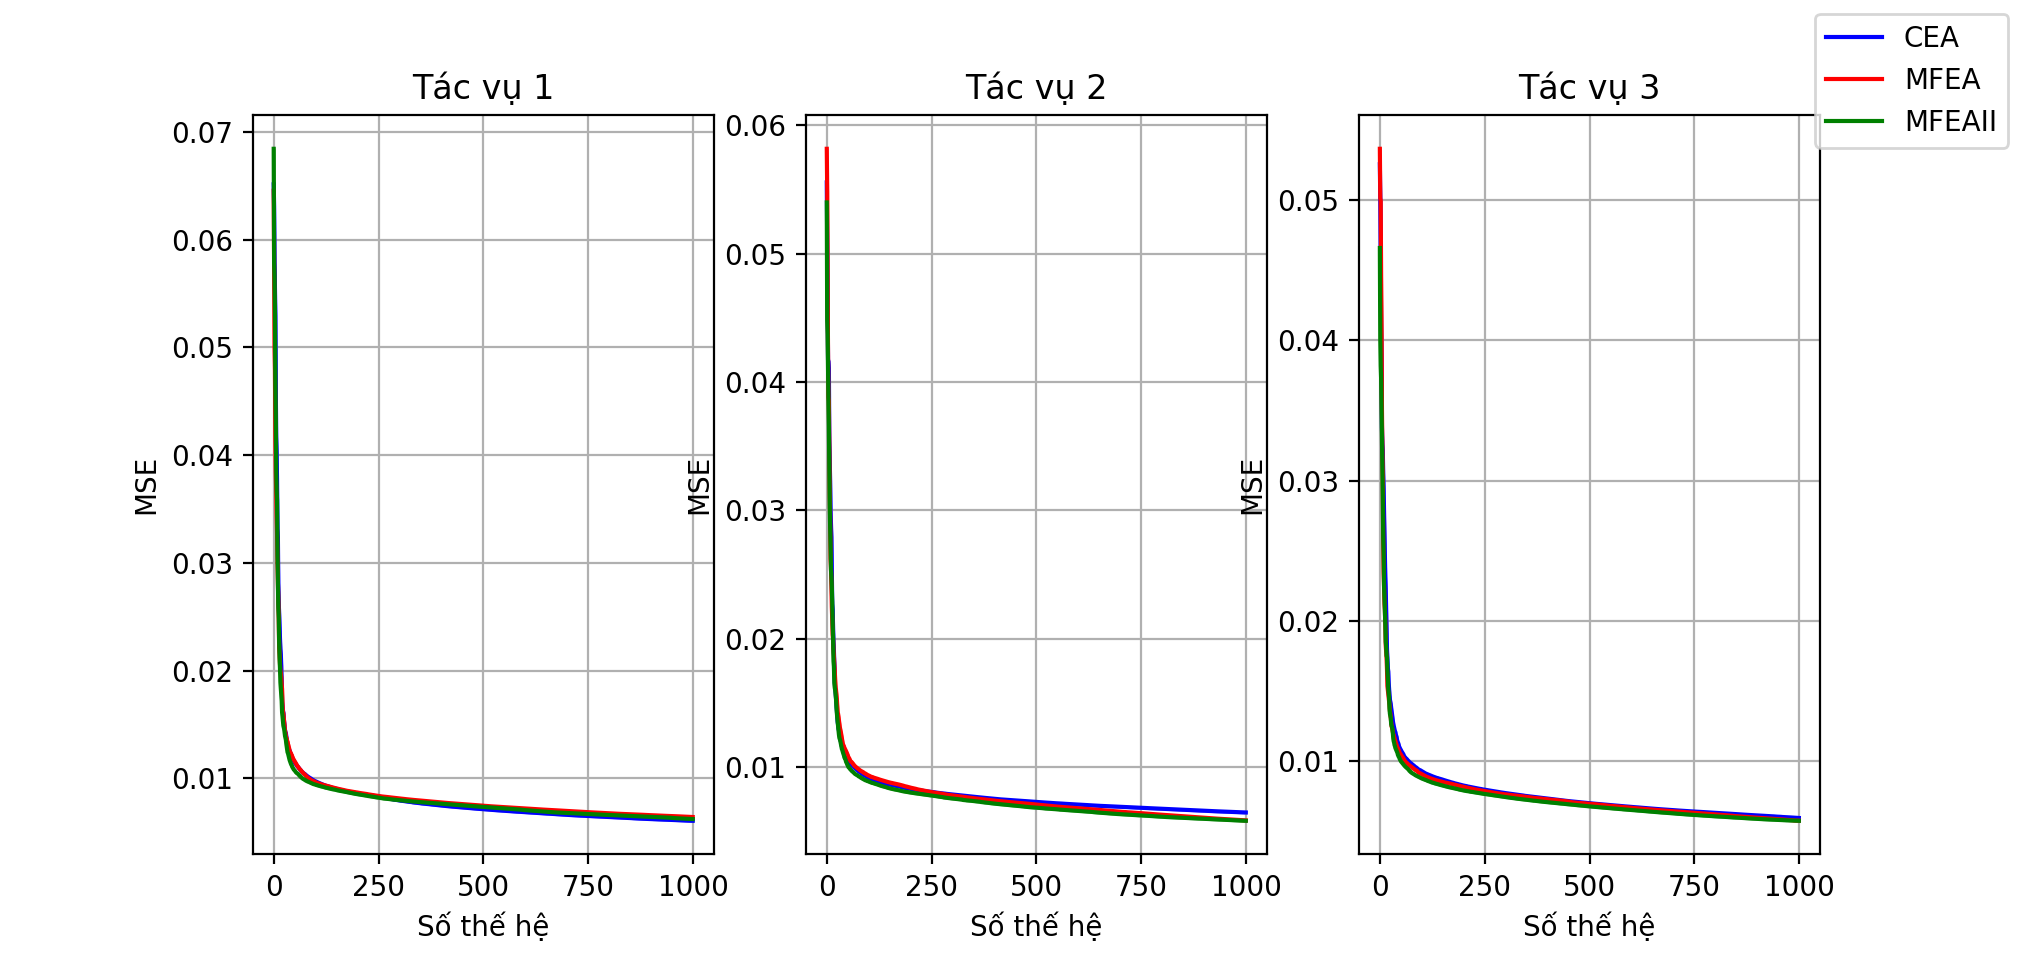
\includegraphics[width=\textwidth,height=\textheight,keepaspectratio]{thesis/images/results/uci/br1_task.png}}
    \scalebox{.7}{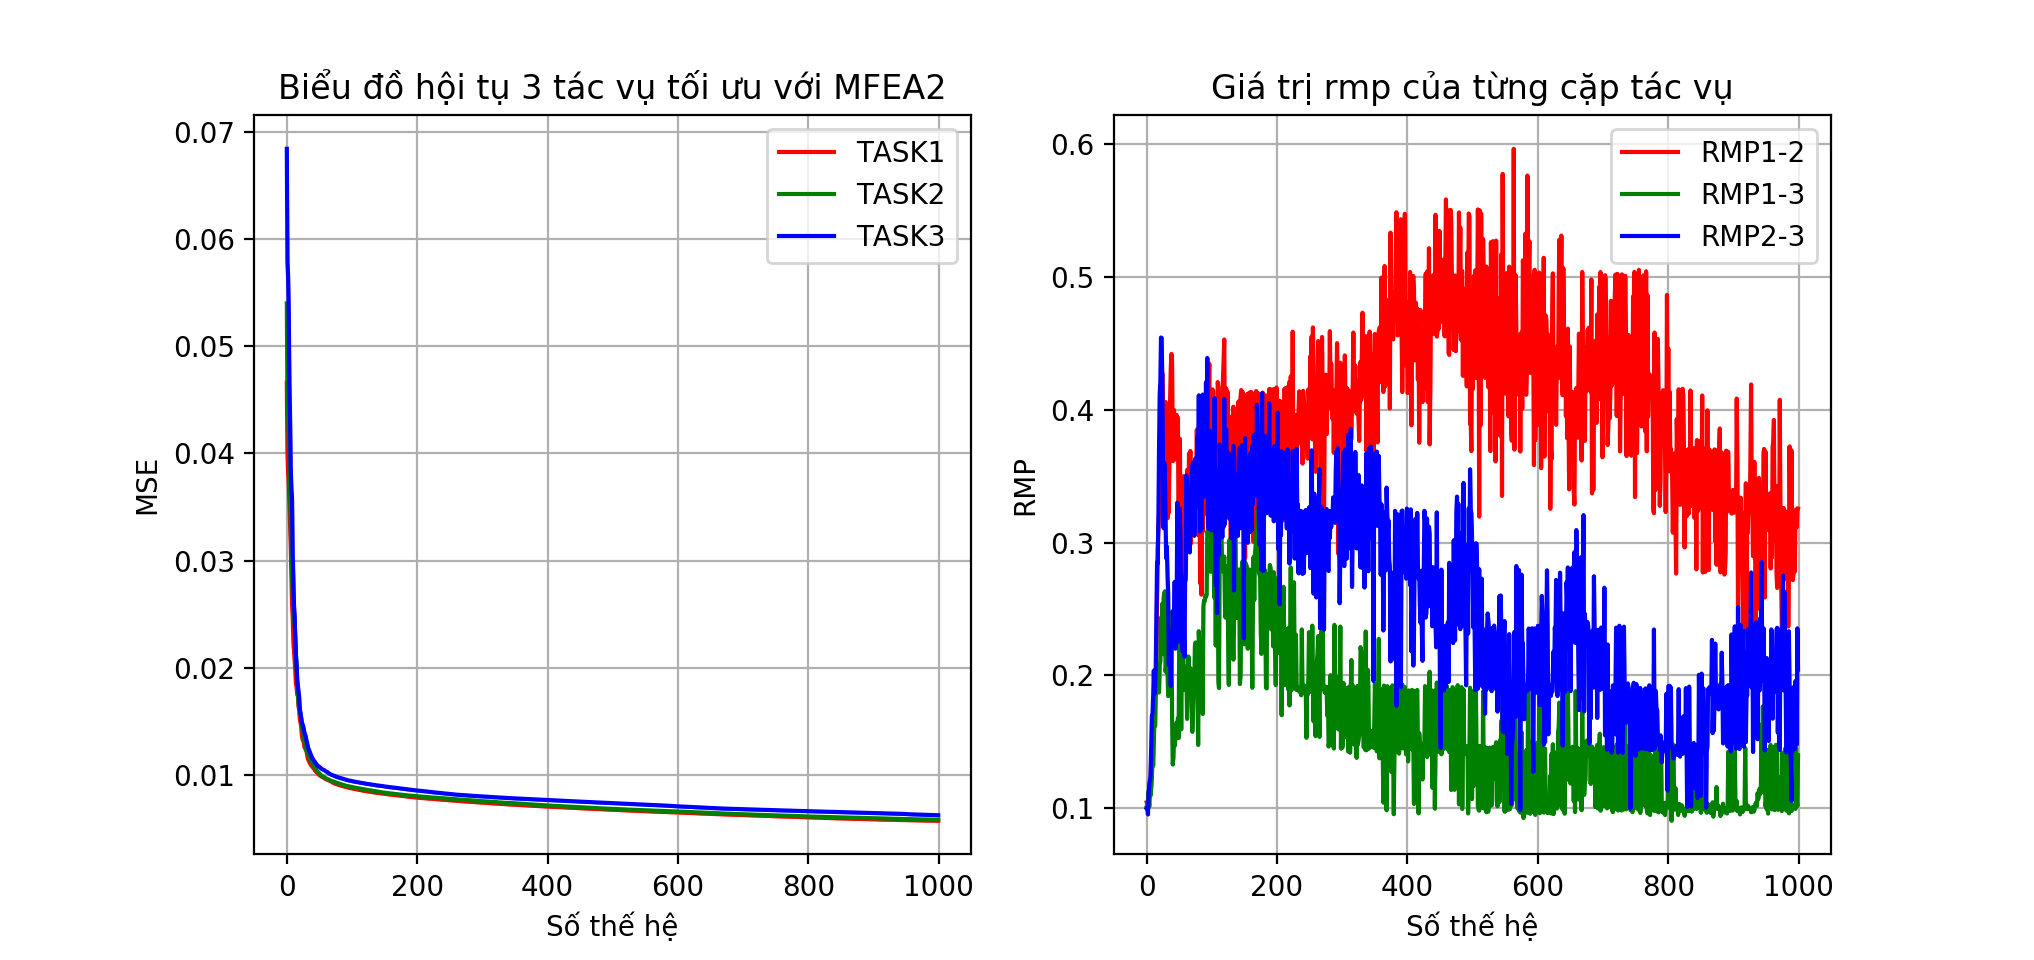
\includegraphics[width=\textwidth,height=\textheight,keepaspectratio]{thesis/images/results/uci/br1_rmp.png}}
    \caption{Biểu đồ hội tụ của các tác vụ bài BreastCancer cùng độ sâu}
    \label{fig:br_mtl}
\end{figure}

\begin{figure}[h!]
    \centering
    \scalebox{.7}{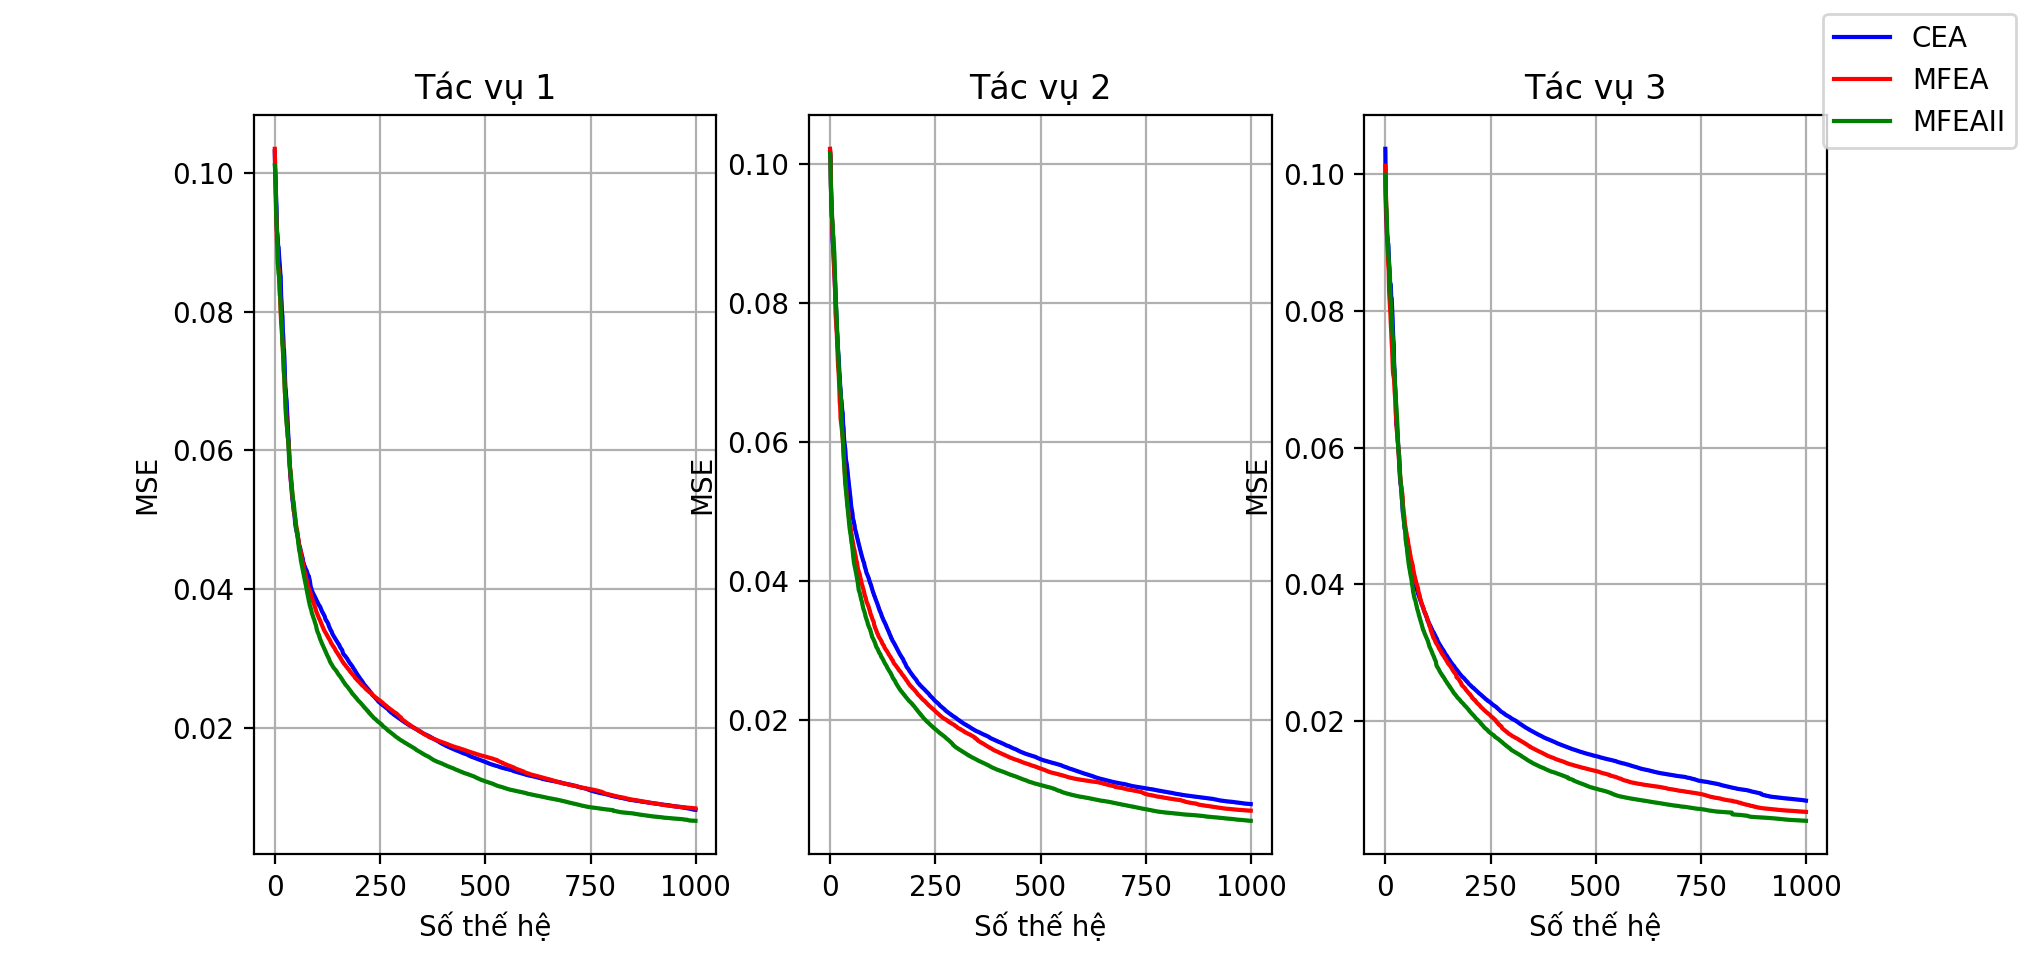
\includegraphics[width=\textwidth,height=\textheight,keepaspectratio]{thesis/images/results/uci/is1_task.png}}
    \scalebox{.7}{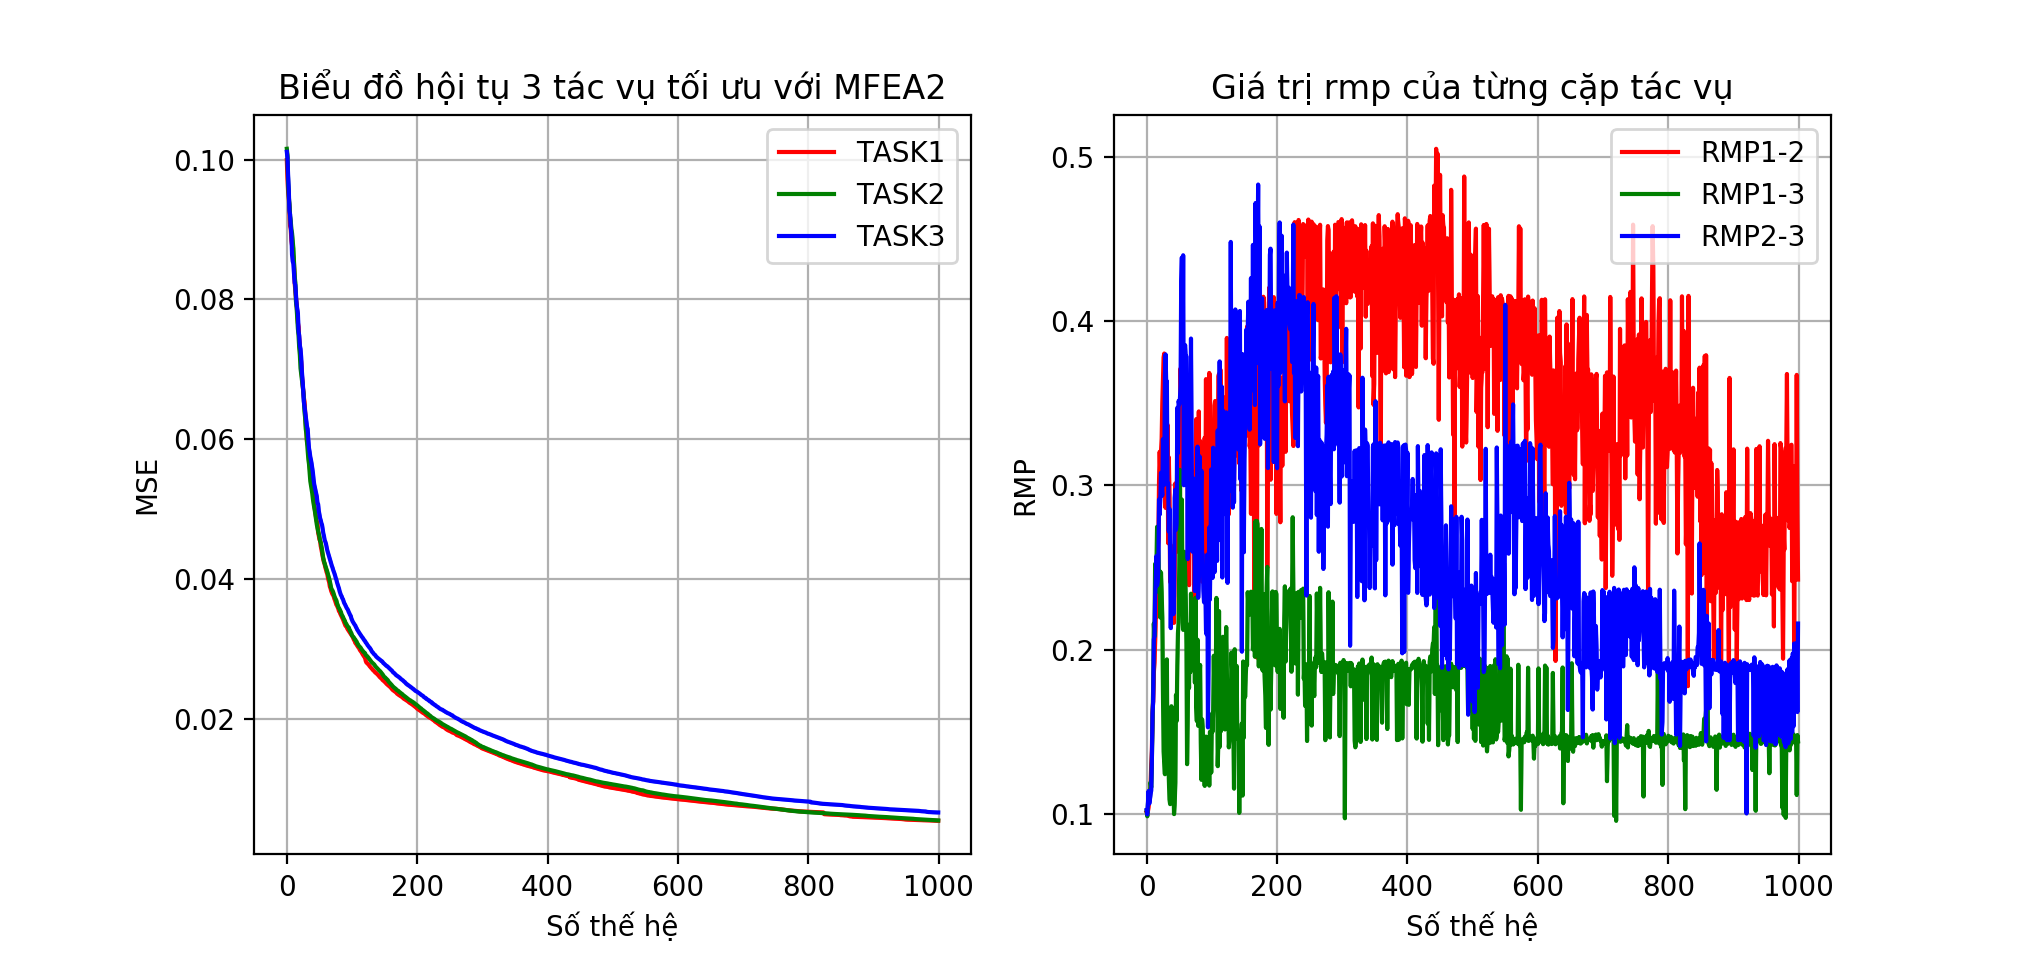
\includegraphics[width=\textwidth,height=\textheight,keepaspectratio]{thesis/images/results/uci/is1_rmp.png}}
    \caption{Biểu đồ hội tụ của các tác vụ bài Ionosphere cùng độ sâu}
    \label{fig:br_mtl}
\end{figure}
\newpage
\subsubsection{Bảng kết quả thực nghiệm - bộ dữ liệu UCI với mạng neural khác độ sâu}
% \begin{table}[h!]
%     \caption{Huấn luyện nhiều ANN trên bộ dữ liệu UCI khác độ sâu}
%     \begin{tabular}{|c|c|c|c|c|}
%     \hline
%     \multirow{1}{*}{\textbf{Instance}} & \multicolumn{1}{c|} {\textbf{Method}} & \multicolumn{1}{c|}{\textbf{Subtask1}} & \multicolumn{1}{c|}{\textbf{Subtask 2}} & \multicolumn{1}{c|}{\textbf{Subtask 3}} \\ \hline
%     \multirow{3}{*} 
%     {breastCancer} & CEA & $0.0119 \pm 0.0029$ & $0.0107 \pm 0.002$ & $\mathbf{0.0093 \pm 0.0005}$ \\
%      & MFEA-I & $\mathbf{0.011 \pm 0.0015}$ & $0.0102 \pm 0.0012$ & $0.0094 \pm 0.0005$  \\ 
%     & MFEA II & $\mathbf{0.011 \pm 0.0015}$ & $\mathbf{0.01 \pm 0.0011}$ & $0.0096 \pm 0.0011$ \\ \hline
    
%     \multirow{3}{*} {creditScreening} & CEA & $0.054 \pm 0.0071$ & $0.0503 \pm 0.0027$ & $0.0485 \pm 0.0017$ \\
%   & MFEA-I & $\mathbf{0.0508 \pm 0.0023}$ & $0.0497 \pm 0.0019$ & $0.0496 \pm 0.0021$ \\ 
%   & MFEA-II & $0.0515 \pm 0.0033$ & $\mathbf{0.0494 \pm 0.0023}$ & $\mathbf{0.0485 \pm 0.0018}$ \\ \hline
   
%     \multirow{3}{*} {ionosphere} & CEA & $0.0516 \pm 0.0124$ & $0.0449 \pm 0.0114$ & $0.0366 \pm 0.0094$ \\
%     &MFEA-I & $0.049 \pm 0.0131$ & $0.0413 \pm 0.0112$ & $\mathbf{0.0365 \pm 0.007}$ \\
%     &MFEA-II & $\mathbf{0.0473 \pm 0.0083}$ & $\mathbf{0.0387 \pm 0.0109}$ & $0.0367 \pm 0.008$  \\\hline
    
%     \multirow{3}{*} {ticTacToe} & CEA & $0.0899 \pm 0.0067$ & $0.0879 \pm 0.0079$ & $0.0852 \pm 0.0045$  \\
%     &MFEA-I & $\mathbf{0.088 \pm 0.008}$ & $0.0886 \pm 0.0064$ & $0.0843 \pm 0.0092$  \\
%     &MFEA-II & $\mathbf{0.088 \pm 0.0073}$ & $\mathbf{0.0832 \pm 0.0067}$ & $0\mathbf{.0817 \pm 0.0046}$  \\\hline
    
%     \end{tabular}

%     \label{tab:result:nbit}
% \end{table}
\begin{table}[h!]
    \caption{Kết quả huấn luyện nhiều ANN trên bộ dữ liệu UCI khác độ sâu}
    \begin{tabular}{|c|c|c|c|c|}
    \hline
    \multirow{1}{*}{\textbf{Instance}} & \multicolumn{1}{c|} {\textbf{Method}} & \multicolumn{1}{c|}{\textbf{Subtask1}} & \multicolumn{1}{c|}{\textbf{Subtask 2}} & \multicolumn{1}{c|}{\textbf{Subtask 3}} \\ \hline
    \multirow{3}{*} 
    {breastCancer} & CEA & $0.0082 \pm 0.0006$ & $0.0083 \pm 0.0006$ & $0.008 \pm 0.0004$ \\
     & MFEA-I & $0.0084 \pm 0.0007$ & $0.0081 \pm 0.0006$ & $0.008 \pm 0.0004$  \\ 
    & MFEA II & $\mathbf{0.0082 \pm 0.0006}$ & $\mathbf{0.008 \pm 0.0004}$ & $\mathbf{0.008 \pm 0.0004}$ \\ \hline
    
    \multirow{3}{*} {creditScreening} & CEA & $0.0442 \pm 0.0016$ & $0.0436 \pm 0.0011$ & $0.0435 \pm 0.0011$ \\
   & MFEA-I & $0.0446 \pm 0.0017$ & $\mathbf{0.0435 \pm 0.0012}$ & $0.0438 \pm 0.0013$ \\ 
   & MFEA-II & $\mathbf{0.0442 \pm 0.0016}$ & $0.0437 \pm 0.0014$ & $\mathbf{0.0433 \pm 0.0012}$ \\ \hline
   
    \multirow{3}{*} {ionosphere} & CEA & $\mathbf{0.0223 \pm 0.0064}$ & $\mathbf{0.0189 \pm 0.005}$ & $\mathbf{0.018 \pm 0.0063}$ \\
    &MFEA-I & $0.0257 \pm 0.01$ & $0.0213 \pm 0.0082$ & $0.0201 \pm 0.0076$ \\
    &MFEA-II & $0.0243 \pm 0.0055$ & $0.0199 \pm 0.0055$ & $0.0203 \pm 0.0062$  \\\hline
    
    \multirow{3}{*} {ticTacToe} & CEA & $0.0747 \pm 0.0077$ & $0.0728 \pm 0.0093$ & $0.0731 \pm 0.0061$   \\
    &MFEA-I & $0.0736 \pm 0.0103$ & $0.0724 \pm 0.008$ & $0.0704 \pm 0.0067$   \\
    &MFEA-II & $\mathbf{0.0709 \pm 0.0096}$ & $\mathbf{0.0667 \pm 0.0066}$ & $\mathbf{0.0684 \pm 0.0067}$  \\\hline
    
    \end{tabular}

    \label{tab:result:nbit}
\end{table}

\newpage
\subsubsection{Biểu đồ hội tụ - bộ dữ liệu UCI với mạng neural cùng độ sâu}

\begin{figure}[h!]
    \centering
    \scalebox{.7}{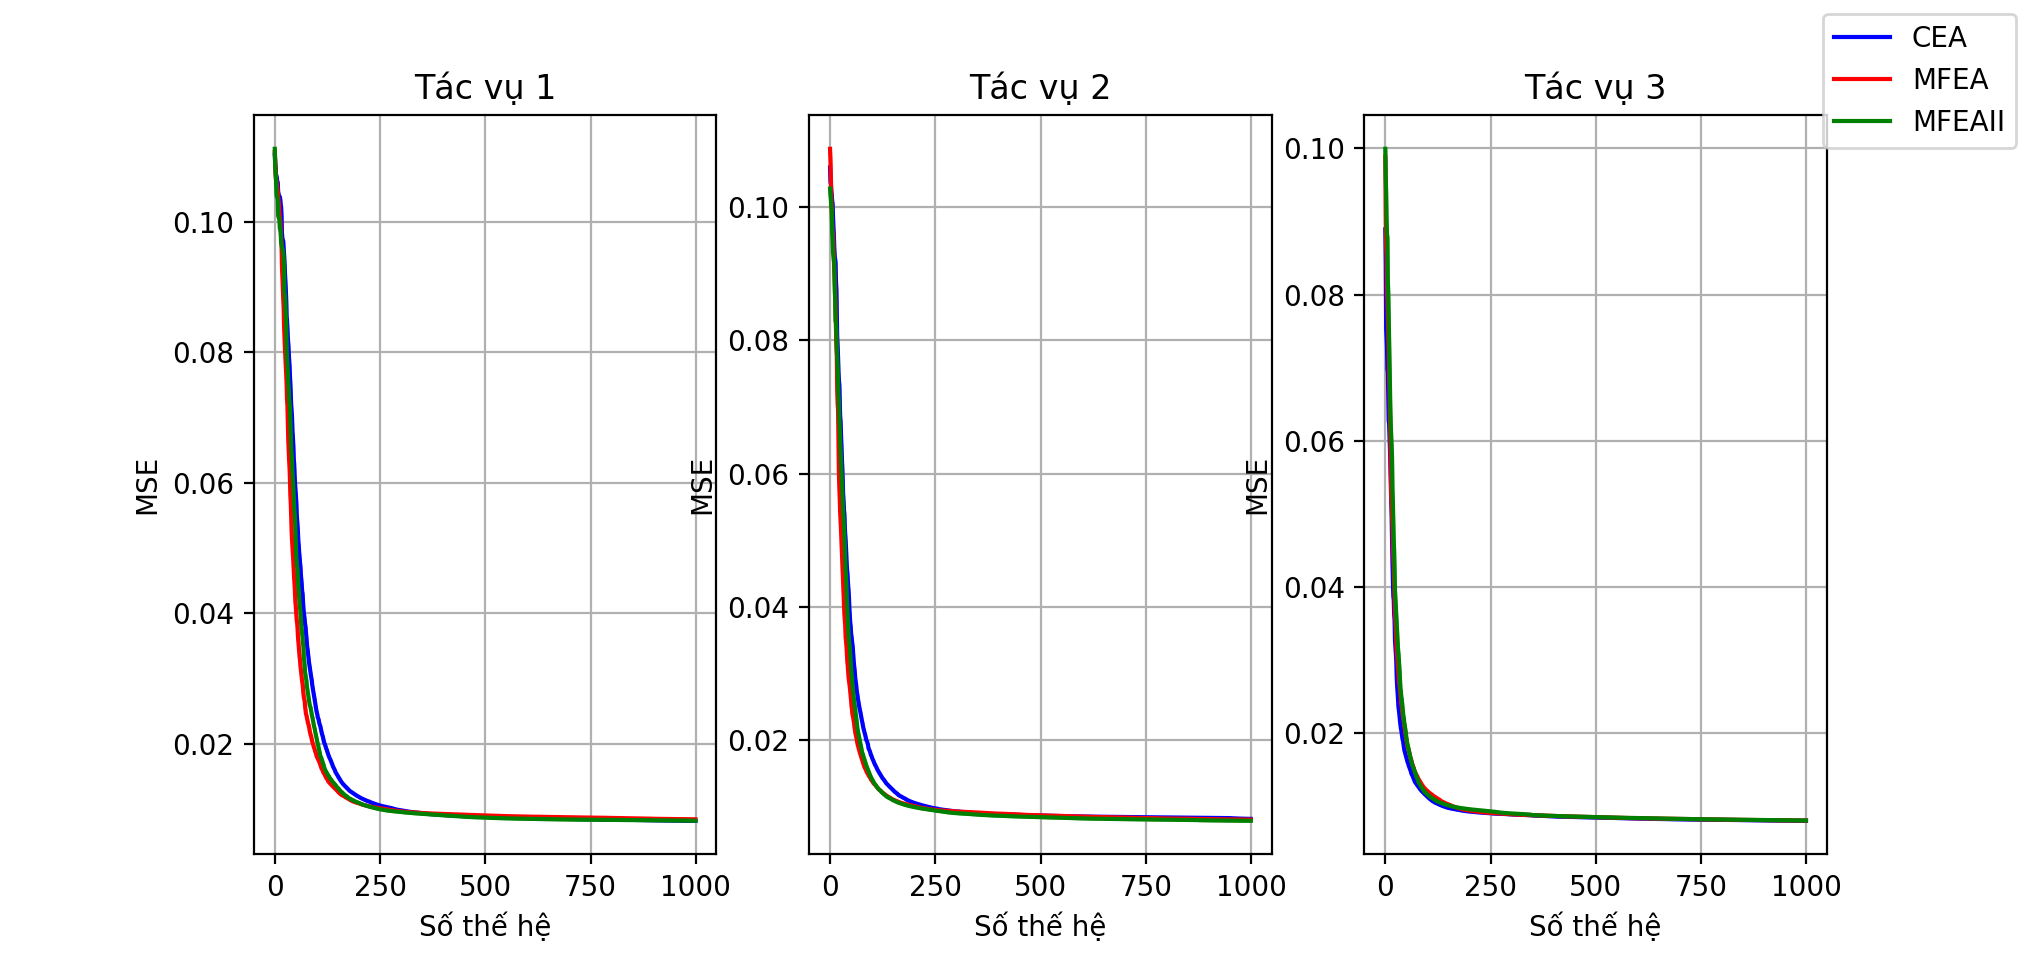
\includegraphics[width=\textwidth,height=\textheight,keepaspectratio]{thesis/images/results/uci/br_task.png}}
    \scalebox{.7}{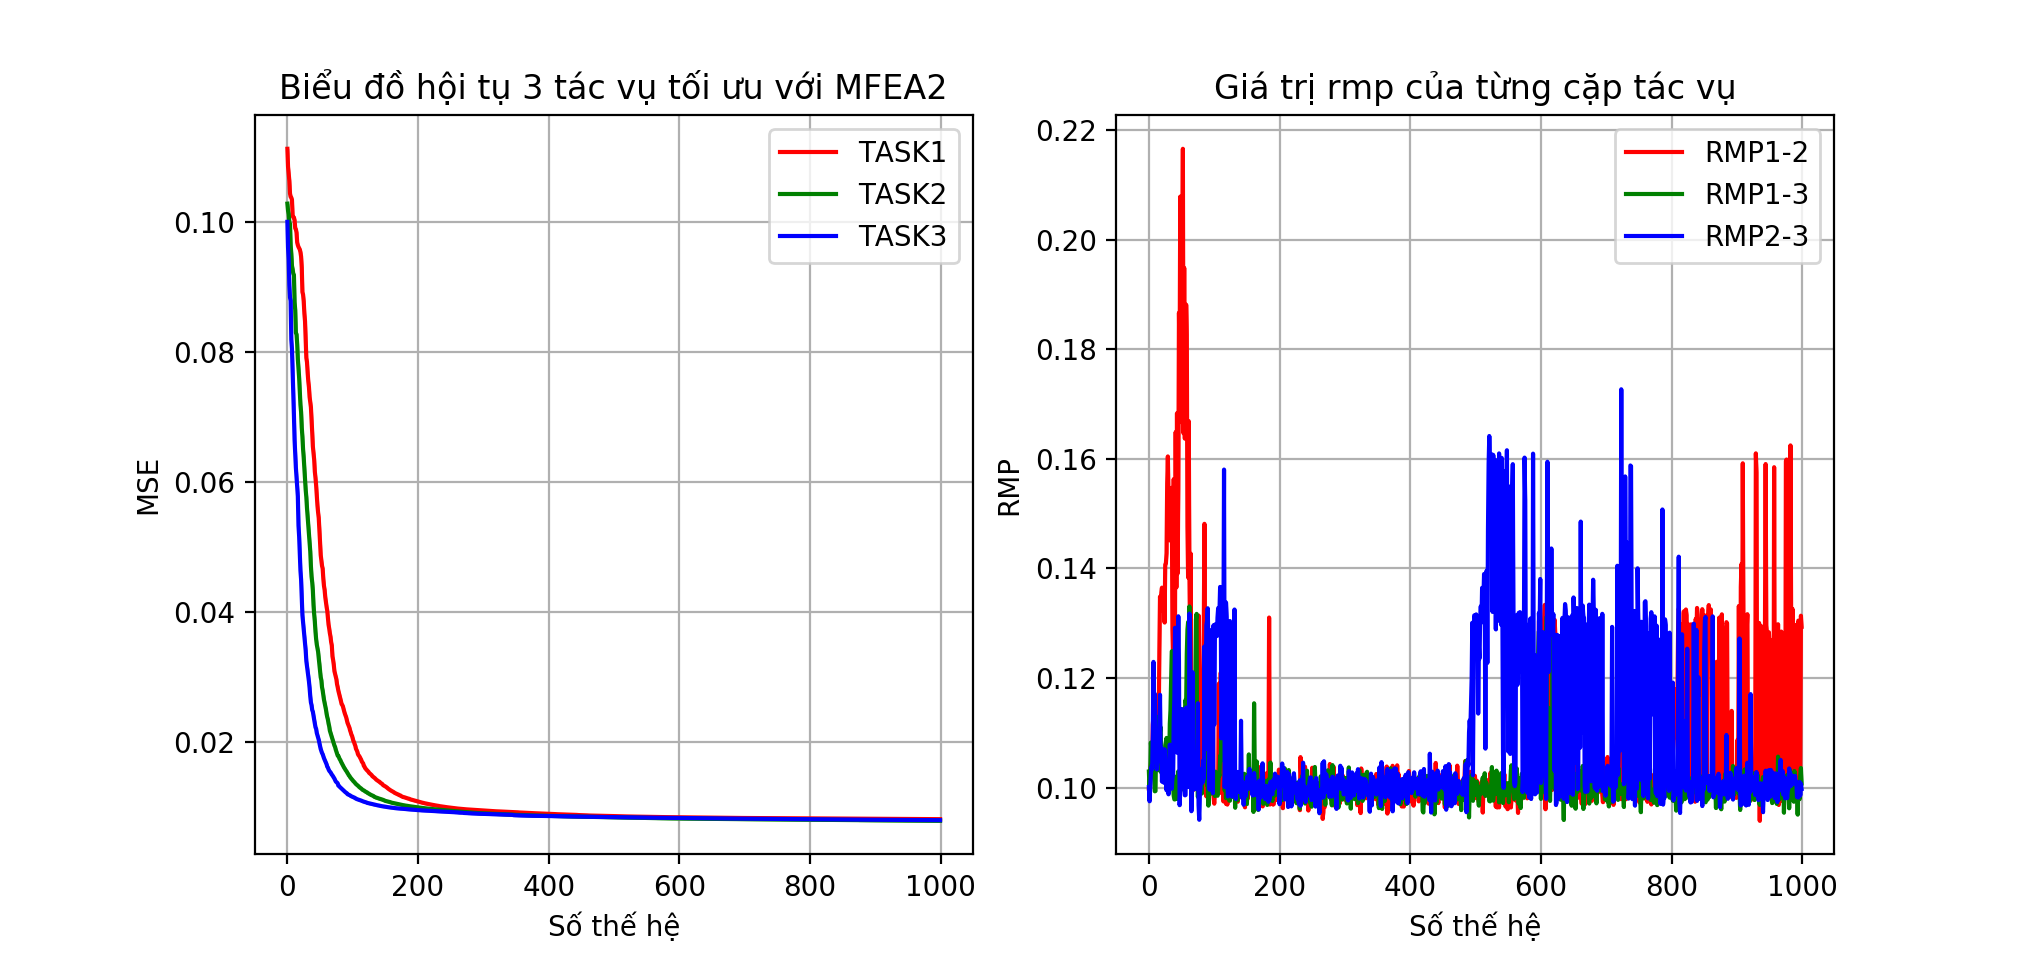
\includegraphics[width=\textwidth,height=\textheight,keepaspectratio]{thesis/images/results/uci/br_rmp.png}}
    \caption{Biểu đồ hội tụ bài BreastCancer khác độ sâu}
    \label{fig:br_mtl}
\end{figure}

\begin{figure}[h!]
    \centering
    \scalebox{.7}{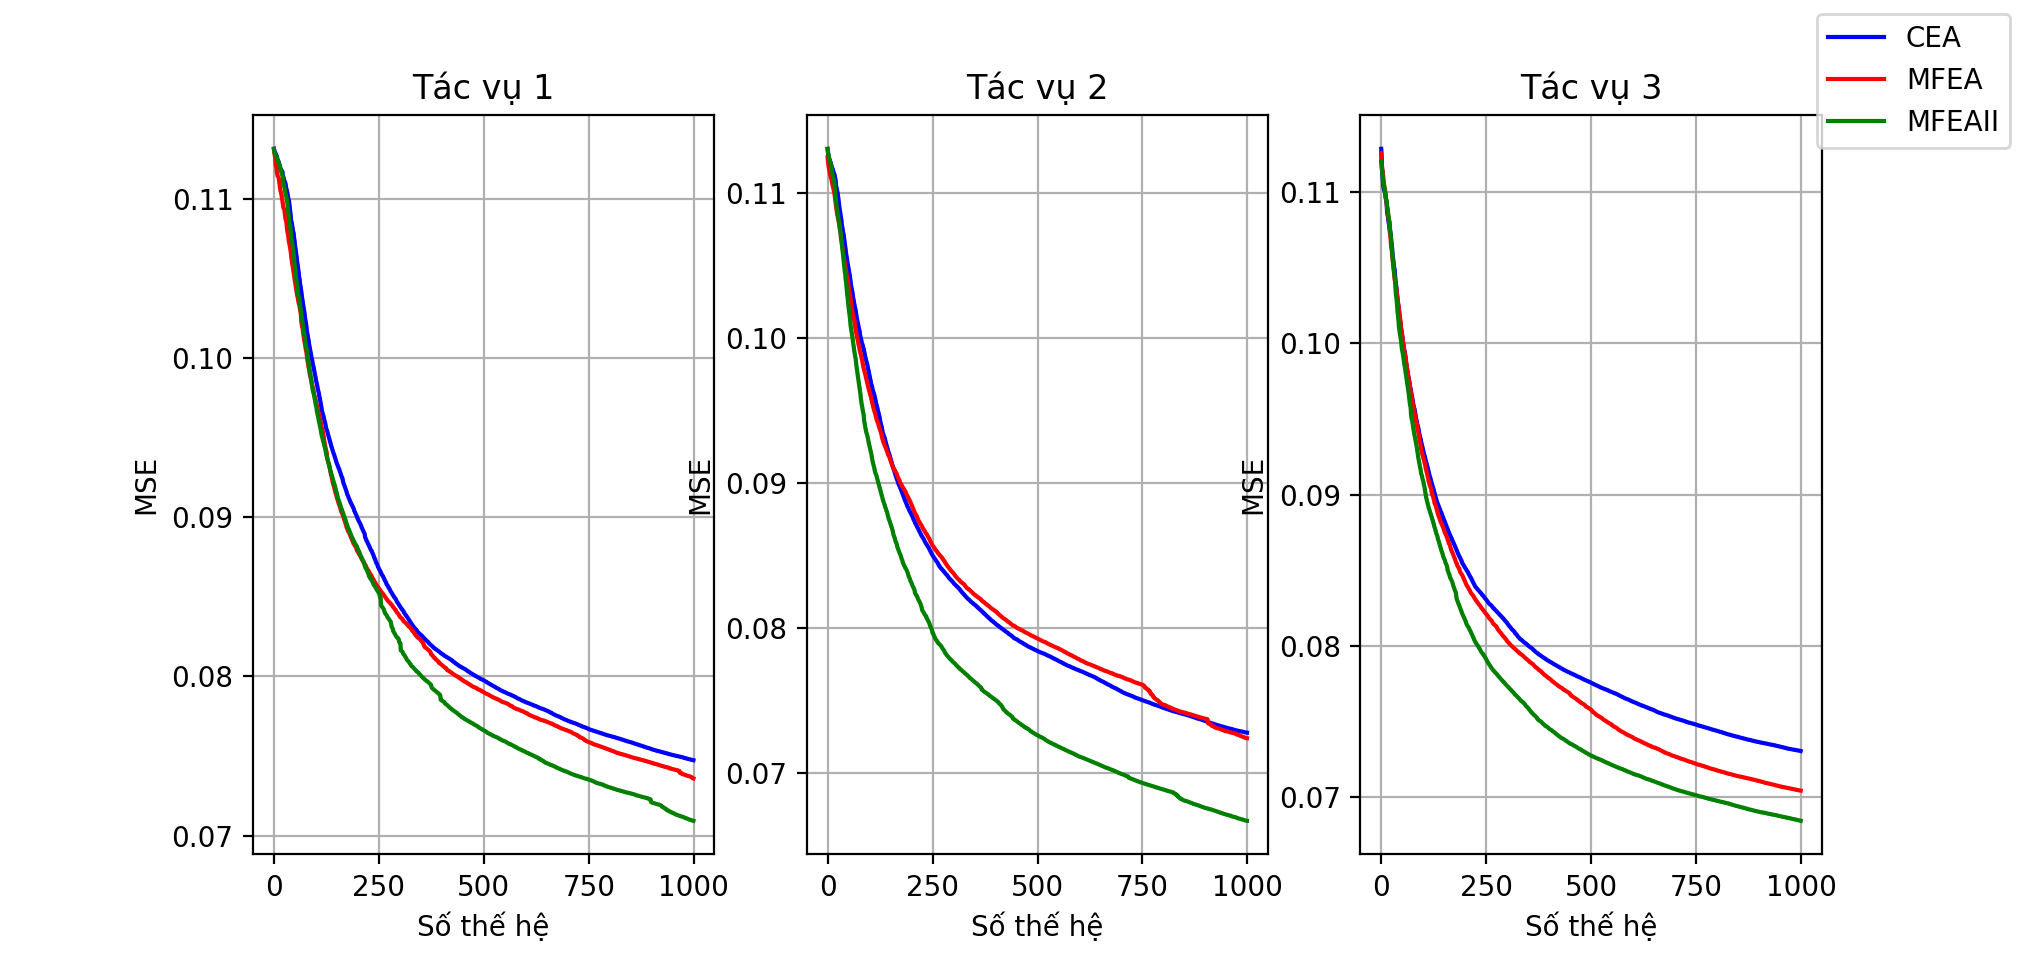
\includegraphics[width=\textwidth,height=\textheight,keepaspectratio]{thesis/images/results/uci/tt_task.png}}
    \scalebox{.7}{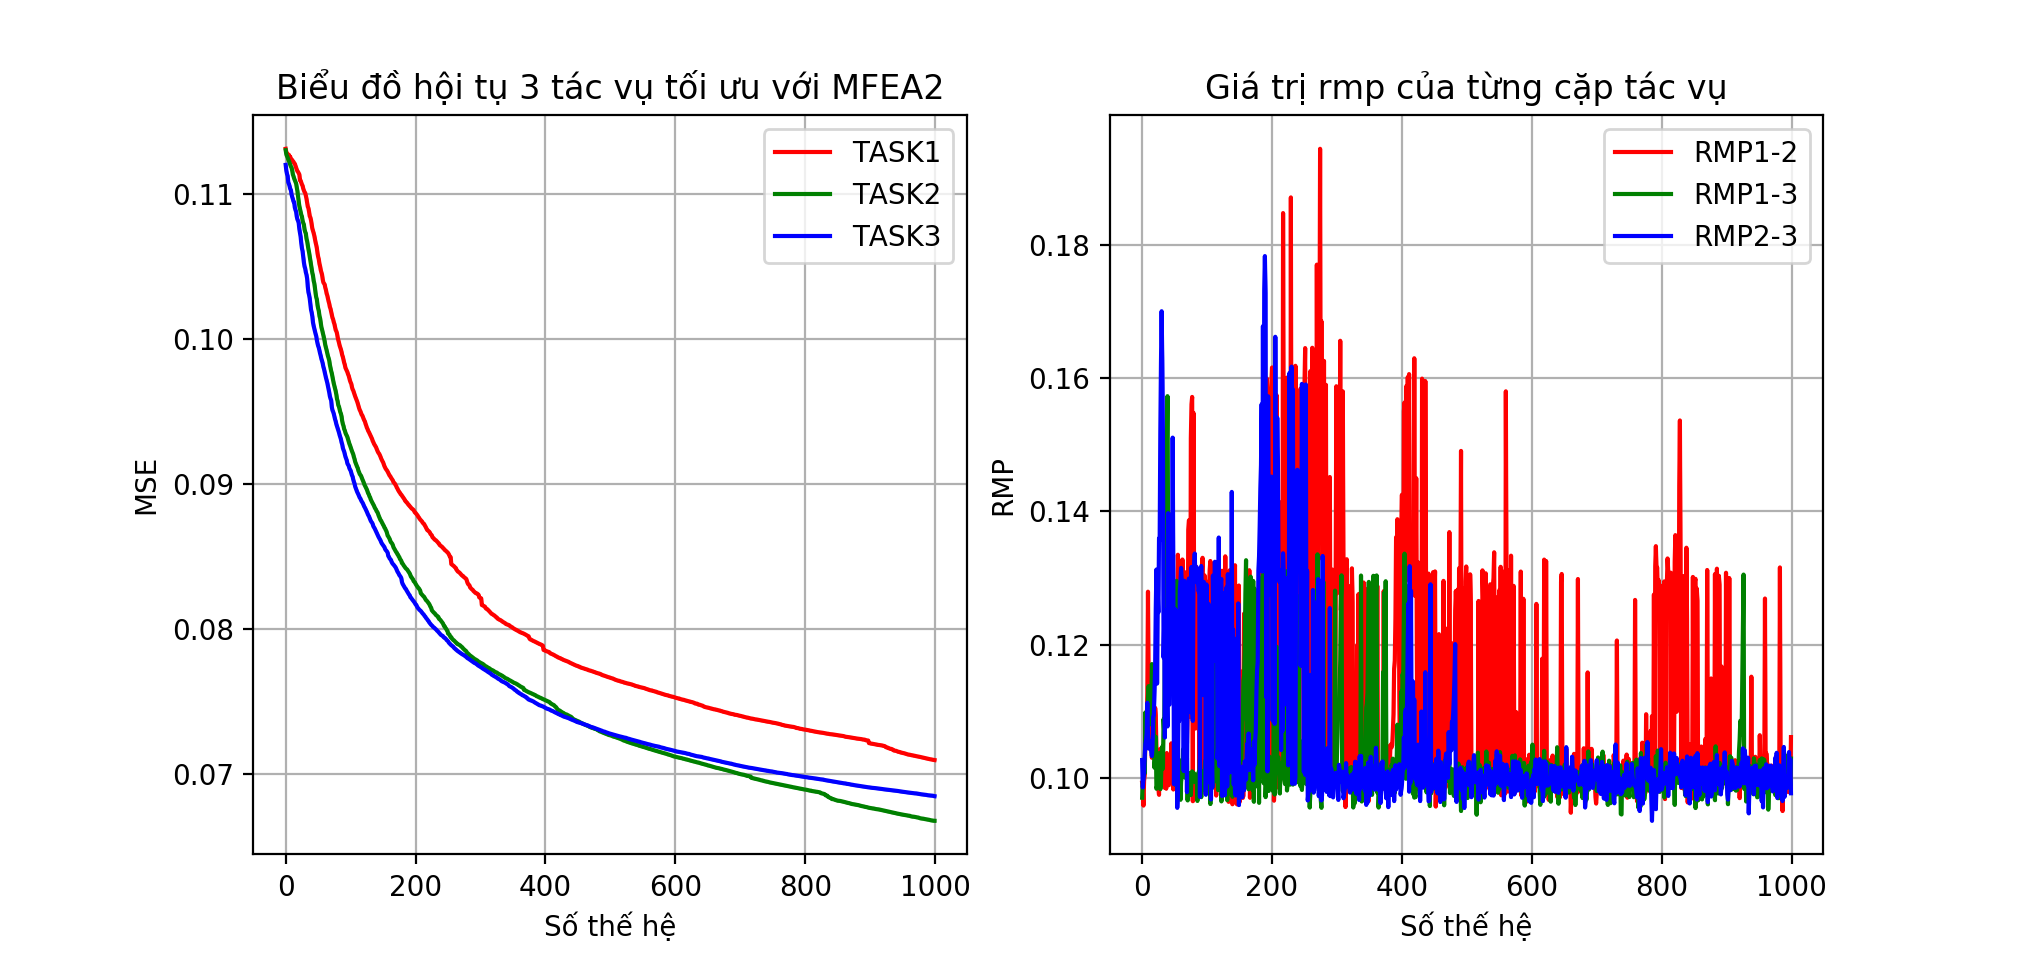
\includegraphics[width=\textwidth,height=\textheight,keepaspectratio]{thesis/images/results/uci/tt_rmp.png}}
    \caption{Biểu đồ hội tụ bài Tictactoe khác độ sâu}
    \label{fig:br_mtl}
\end{figure}
\pagebreak

\subsection{Kết quả huấn luyện trên các môi trường học tăng cường}
% \begin{table}
%     \caption{Mô hình học tăng cường khác môi trường}
%     \begin{center}
%     \begin{tabular}{|c|c|c|c|c|c|}
%     \hline
%     \multirow{1}{*}{\textbf{Trọng lực}} &
%     \multirow{1}{*}{\textbf{Method}} & \multicolumn{1}{c|}{\textbf{Cao nhất}} & {\textbf{Thấp nhất}} & \multicolumn{1}{c|}{\textbf{Trung Bình}} & \multicolumn{1}{c|}{\textbf{Độ lệch}} \\ \hline
%     \multirow{3}{*} 
%     {Trọng lực=1.0} &
%     CEA & $71$ & $4$ & $28.86$ & $17.16$ \\
%     & MFEAI & $\mathbf{129}$ & $17$ &$46.71$ & $20.36$  \\
%     & MFEAII & $84$ & $15$ & $\mathbf{52.81}$  &$15.45$\\\hline
%     \multirow{3}{*} 
%     {Trọng lực=1.98} &
%     CEA & $382$ & $7$ &$174.86$ & $113.79$ \\
%     & MFEAI  & $\mathbf{546}$ & $98$ & $\mathbf{319.86}$ & $95.34$ \\
%     & MFEAII & $517$ & $\mathbf{131}$ &$311.38$ & $106.76$ \\\hline
%     \multirow{3}{*} 
%     {Trọng lực=2.96} &
%     CEA & $272$ & $1$ &$97.9$ & $83.07$ \\
%     & MFEAI  & $\mathbf{349}$ & $\mathbf{140}$ & $\mathbf{222.81}$ & $52.07$ \\
%     & MFEAII & $322$ & $103$ &$212.38$ & $52.74$ \\\hline
%     \multirow{3}{*} 
%     {Trọng lực=3.94} &
%     CEA & $227$ & $2$ &$69.24$ & $56.64$ \\
%     & MFEAI  & $\mathbf{217}$ & $\mathbf{95}$ & $\mathbf{142.86}$ & $27.4$ \\
%     & MFEAII & $190$ & $76$ &$140.38$ & $27.78$ \\\hline
%     \multirow{3}{*} 
%     {Trọng lực=4.92} &
%     CEA & $95$ & $2$ & $25.48$ & $25.78$  \\
%     & MFEAI  & $\mathbf{181}$ & $\mathbf{54}$ & $90.86$ & $21.98$ \\
%     & MFEAII & $145$ & $44$ & $\mathbf{102.14}$ & $26.66$ \\\hline
%     \end{tabular}
%     \end{center}
    
%     \label{tab:result:nbit}
% \end{table}

\subsubsection{Bảng kết quả thực nghiệm - bài toán Acrobot}
\begin{table} [H]
    \begin{center}
    \caption{Kết quả huấn luyện các tác vụ cho bài toán Acrobot}

    \scalebox{0.9}{\begin{tabular}{|c|c|c|c|c|c|}
    \hline
    \multirow{1}{*}{\textbf{Thuật toán}} & \multicolumn{1}{c|}{\textbf{Tác vụ 1}} & \multicolumn{1}{c|}{\textbf{Tác vụ 2}} & \multicolumn{1}{c|}{\textbf{Tác vụ 3}} & \multicolumn{1}{c|}{\textbf{Tác vụ 4}} & \multicolumn{1}{c|}{\textbf{Tác vụ 5}} \\ \hline
    CEA & $-100 \pm 4.53$ & $-109.47 \pm 2.38$ & $-108.77 \pm 4.38$ & $-113.17 \pm 1.86$ & $-117.23 \pm 4.28$  \\
    MFEAI &  $-100 \pm 4.75$ & $\mathbf{-106.7 \pm 0.78}$ & $\mathbf{-108.3 \pm 4.47}$ & $-112.0 \pm 2.62$ & $-117.03 \pm 4.52$ \\
    MFEAII & $\mathbf{-100 \pm 4.7}$ & $-107.8 \pm 1.17$ & $-108.6 \pm 4.34$ & $\mathbf{-113.07 \pm 2.29}$ & $\mathbf{-116.9 \pm 4.09}$  \\\hline
    \end{tabular}}
    \end{center}
    \label{tab:result:acrobot}
\end{table}


\subsubsection{Biểu đồ hội tụ - bài toán Acrobot}
\begin{figure}[h!]
    \centering
    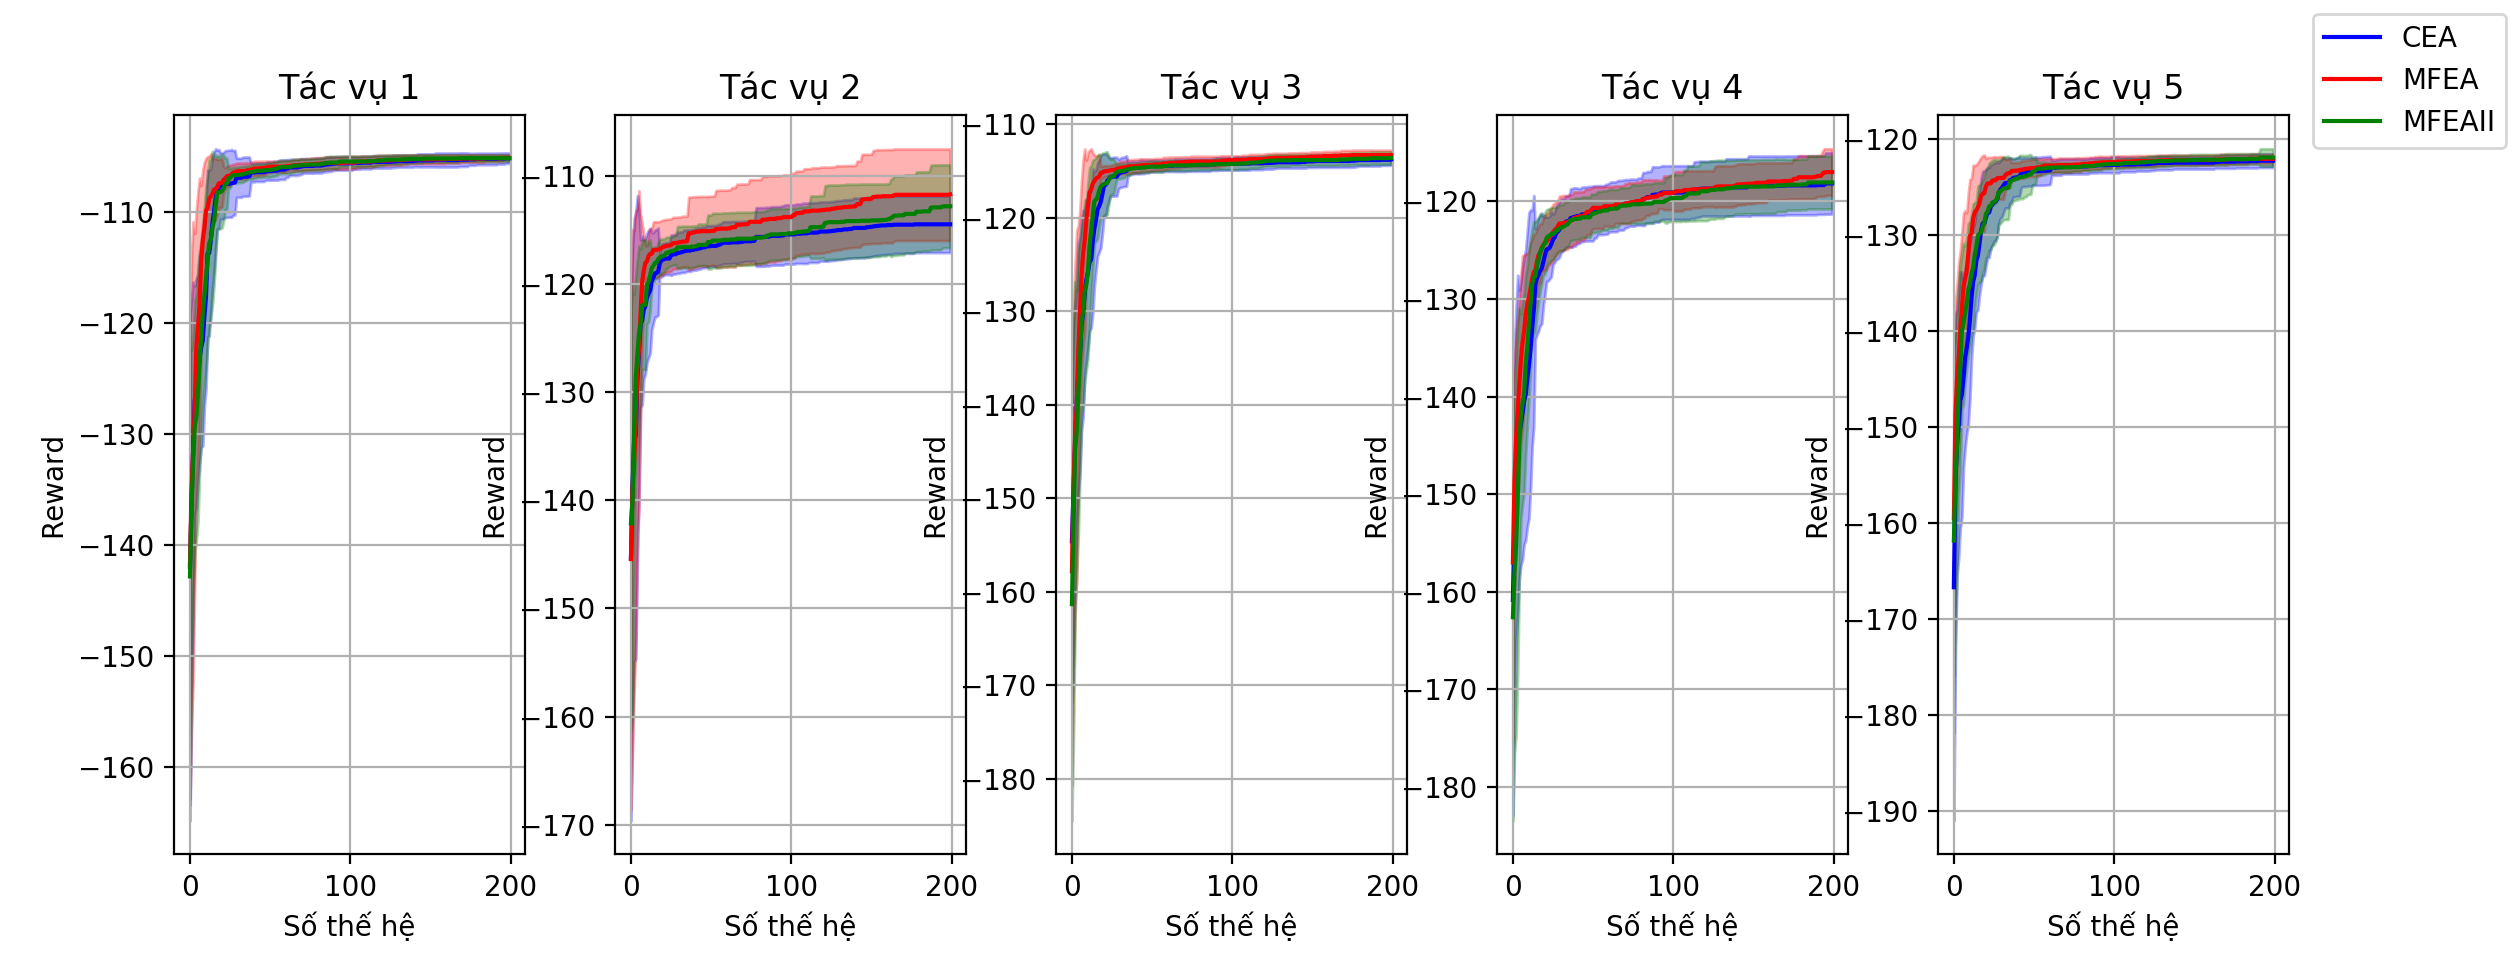
\includegraphics[width=\textwidth,height=\textheight,keepaspectratio]{thesis/images/results/rl/acrobot_conv.png}
    \caption{Biểu đồ hội tụ các tác vụ cho bài toán Acrobot}
    \label{fig:Acrobot_conv}
\end{figure}

\subsubsection{So sánh mức độ tập trung kết quả cuối cùng - bài toán Acrobot}
\begin{figure}[h!]
    \centering
    \includegraphics[width=\textwidth,height=\textheight,keepaspectratio]{thesis/images/results/rl/acrobot_final.png}
    \caption{Biểu đồ so sánh mức độ tập trung kết quả cuối cùng cho bài toán Acrobot (khi so sánh trị tuyệt đối của kết quả)}
    \label{fig:Acrobot}
\end{figure}


\subsubsection{Bảng kết quả thực nghiệm - bài toán PixelCopter}
\begin{table} [h!]
    \begin{center}
    \caption{Kết quả huấn luyện các tác vụ cho bài toán PixelCopter}

    \scalebox{0.9}{\begin{tabular}{|c|c|c|c|c|c|}
    \hline
    \multirow{1}{*}{\textbf{Thuật toán}} & \multicolumn{1}{c|}{\textbf{Tác vụ 1}} & \multicolumn{1}{c|}{\textbf{Tác vụ 2}} & \multicolumn{1}{c|}{\textbf{Tác vụ 3}} & \multicolumn{1}{c|}{\textbf{Tác vụ 4}} & \multicolumn{1}{c|}{\textbf{Tác vụ 5}} \\ \hline
    CEA & $101.97 \pm 26.15$ & $104.6 \pm 23.16$ & $96.83 \pm 22.74$ & $96.67 \pm 28.27$ & $93.47 \pm 19.09$ \\
    MFEAI & $124.47 \pm 32.08$ & $125.93 \pm 31.4$ & $123.43 \pm 24.86$ & $122.33 \pm 23.08$ & $120.37 \pm 30.36$  \\
    MFEAII & $\mathbf{133.57 \pm 28.29}$ & $\mathbf{132.03 \pm 33.31}$ & $\mathbf{132.73 \pm 26.93}$ & $\mathbf{129.0 \pm 22.93}$ & $\mathbf{135.4 \pm 30.11}$ \\\hline
    \end{tabular}}
    \end{center}
    \label{tab:result:pixelcopter}
\end{table}


\subsubsection{Biểu đồ hội tụ - bài toán PixelCopter}
\begin{figure}[h!]
    \centering
    \includegraphics[width=\textwidth,height=\textheight,keepaspectratio]{thesis/images/results/rl/pixcelcopter_conv.png}
    \caption{Biểu đồ hội tụ các tác vụ cho bài toán PixelCopter}
    \label{fig:PixelCopter_conv}
\end{figure}

\subsubsection{So sánh mức độ tập trung kết quả cuối cùng - bài toán PixelCopter}
\begin{figure}[h!]
    \centering
    \includegraphics[width=\textwidth,height=\textheight,keepaspectratio]{thesis/images/results/rl/pixelcopter_final.png}
    \caption{Biểu đồ so sánh mức độ tập trung kết quả cuối cùng cho bài toán PixelCopter}
    \label{fig:PixelCopter}
\end{figure}
\subsubsection{Bảng kết quả thực nghiệm - bài toán FlappyBird}
\begin{table} [H]
    \begin{center}
    \caption{Kết quả huấn luyện các tác vụ cho bài toán FlappyBird}

    \scalebox{0.9}{\begin{tabular}{|c|c|c|c|c|c|}
    \hline
    \multirow{1}{*}{\textbf{Thuật toán}} & \multicolumn{1}{c|}{\textbf{Tác vụ 1}} & \multicolumn{1}{c|}{\textbf{Tác vụ 2}} & \multicolumn{1}{c|}{\textbf{Tác vụ 3}} & \multicolumn{1}{c|}{\textbf{Tác vụ 4}} & \multicolumn{1}{c|}{\textbf{Tác vụ 5}} \\ \hline
    CEA & $25.9 \pm 17.57$ & $219.1 \pm 151.39$ & $101.8 \pm 88.65$ & $78.77 \pm 62.43$ & $24.63 \pm 23.62$ \\
    MFEAI & $47.43 \pm 17.97$ & $\mathbf{319.83 \pm 118.9}$ & $\mathbf{217.87 \pm 48.57}$ & $142.9 \pm 26.86$ & $90.17 \pm 20.69$ \\
    MFEAII & $\mathbf{50.93 \pm 16.47}$ & $314.07 \pm 116.25$ & $214.83 \pm 51.96$ & $\mathbf{145.47 \pm 26.72}$ & $\mathbf{105.33 \pm 26.12}$ \\\hline
    \end{tabular}}
    \end{center}
    \label{tab:result:pixelcopter}
\end{table}


\subsubsection{Biểu đồ hội tụ - bài toán FlappyBird}
\begin{figure}[h!]
    \centering
    \includegraphics[width=\textwidth,height=\textheight,keepaspectratio]{thesis/images/results/rl/flappybird_conv.png}
    \caption{Biểu đồ hội tụ các tác vụ cho bài toán FlappyBird}
    \label{fig:FLP_conv}
\end{figure}

\subsubsection{So sánh mức độ tập trung kết quả cuối cùng - bài toán FlappyBird}
\begin{figure}[h!]
    \centering
    \includegraphics[width=\textwidth,height=\textheight,keepaspectratio]{thesis/images/results/rl/flappybird_final.png}
    \caption{Biểu đồ so sánh mức độ tập trung kết quả cuối cùng cho bài toán FlappyBird}
    \label{fig:FLP}
\end{figure}

	
\end{document}